\begin{quoting}
In this chapter, you will learn how to make
freestanding wheat sourdough bread.
\end{quoting}

\begin{figure}[!htb]
  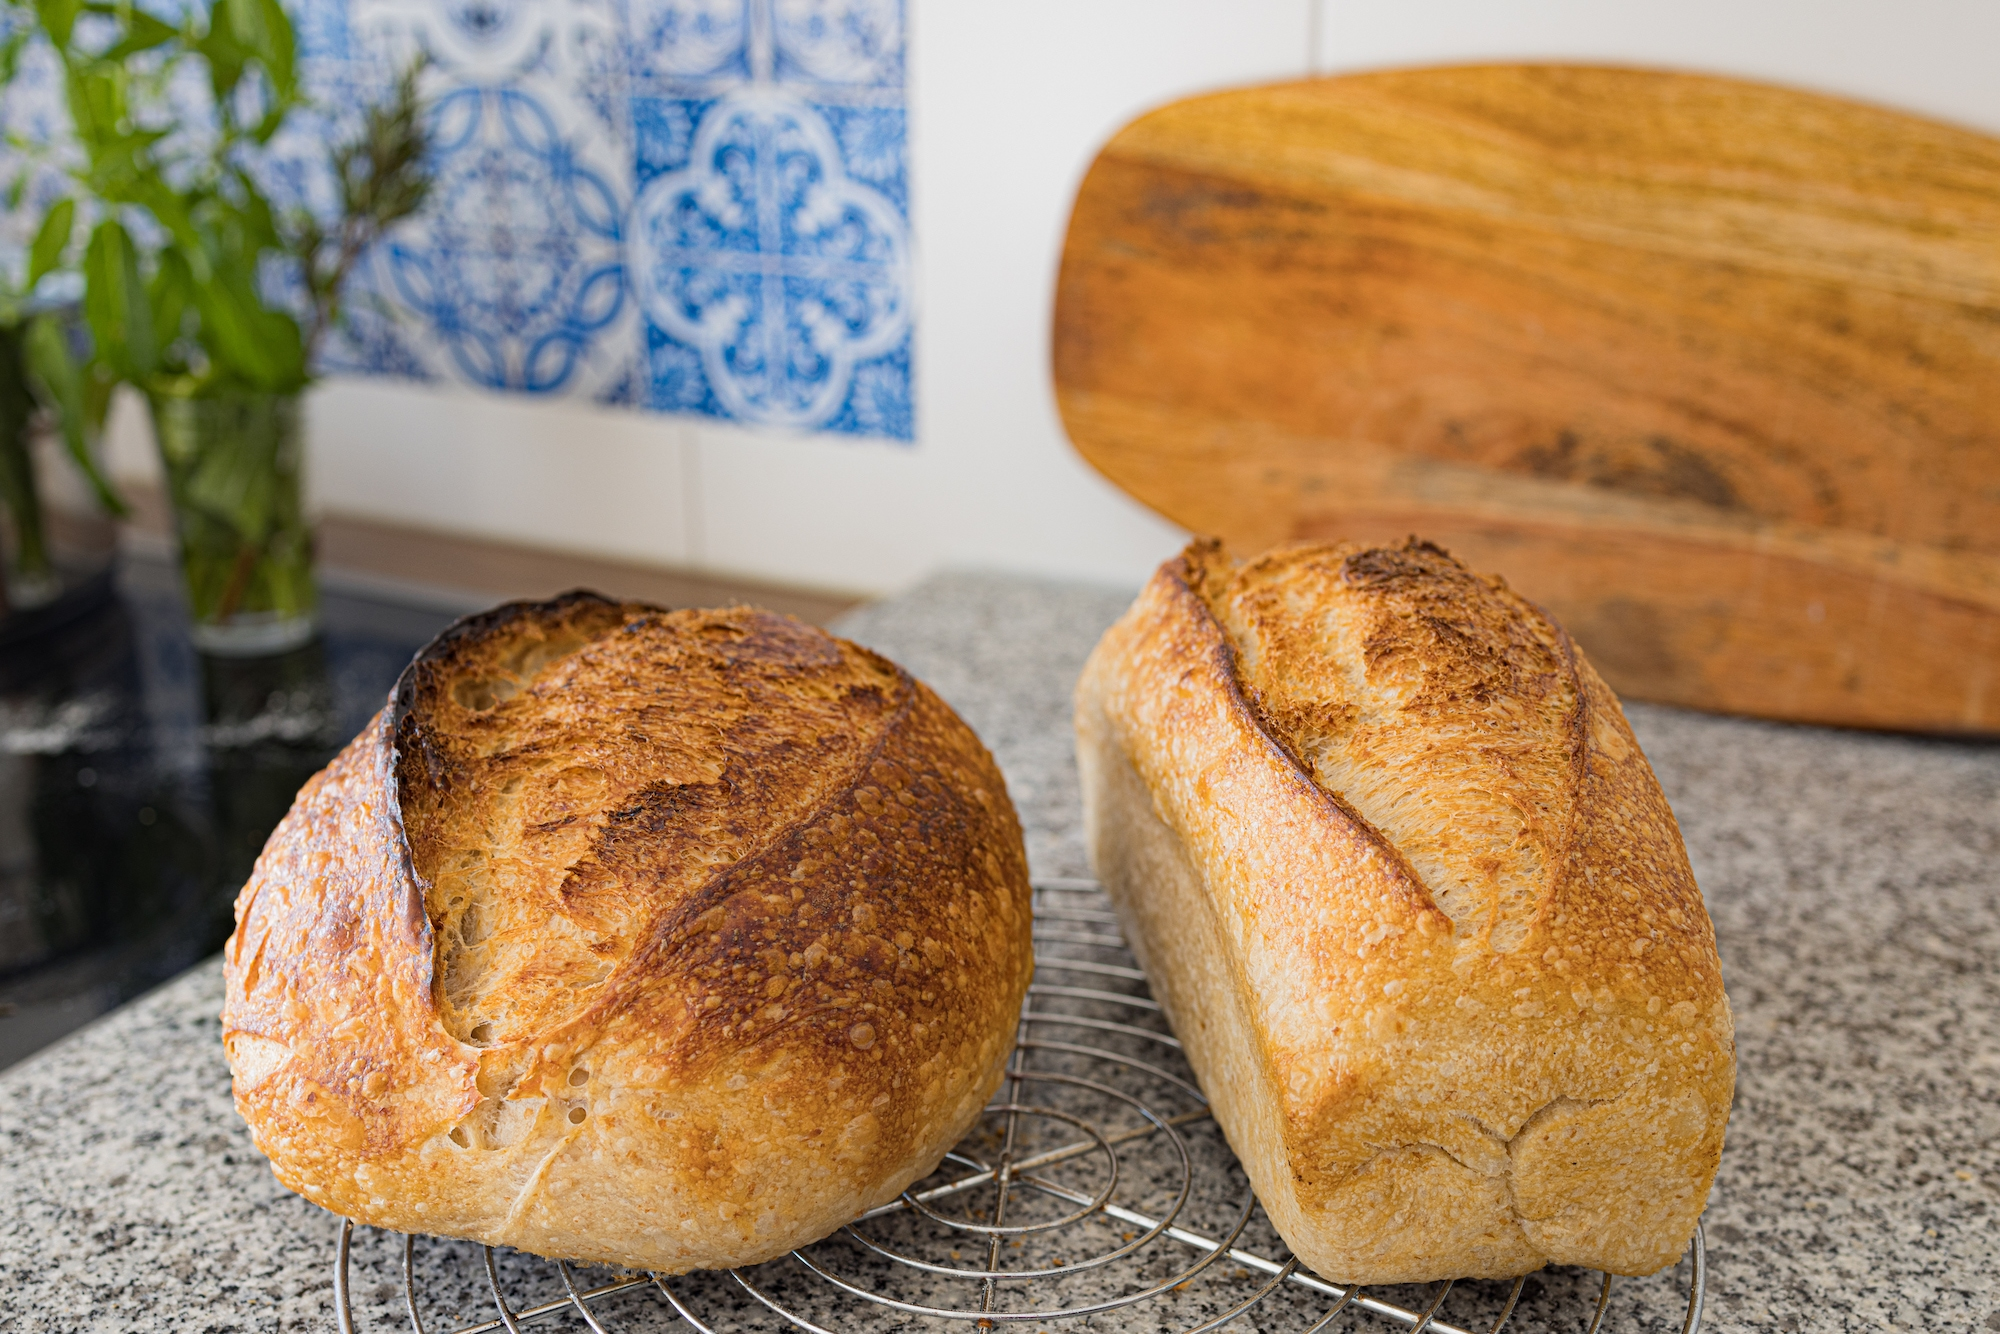
\includegraphics[width=\textwidth]{loaf-pan-free-standing.jpg}
  \caption[Freestanding and loaf pan bread]{A freestanding sourdough bread
      next to bread made in a loaf pan.  Freestanding sourdough is considered
      the supreme discipline of sourdough bread by many bakers.}
\end{figure}

Freestanding sourdough bread is my favorite
type of bread. It combines a great crunchy crust, superb
flavor, and a soft fluffy crumb. This is the type of bread
that is being inhaled by my friends and family. Unfortunately,
making this type of bread requires a lot more effort, patience,
and technique than other types of bread. You have to perfectly
balance the fermentation process. You cannot ferment for too
short and also not for too long. The techniques you need to
learn also require a bit more skill. It took me several attempts
to get this right. I faced several challenges: I~had the wrong flour.
I~didn't properly know how to use my oven.
When should I~stop the fermentation? There is a lot of information
out there. I~dug through most of it and have tried almost everything.
In many cases the information was wrong; in other cases, I~found another
valuable puzzle piece. Aggregating all this
information was one of my main motivations to start \texttt{The Bread Code}.
My key learning was that there is no recipe that
you can blindly follow. You will always have to adapt the recipe
to your locally available tools and environment.

But do not worry. After reading this chapter you will know
all the signs to look out for. You will be able to read your dough.
You will turn into a confident hobby baker who can bake bread
at home, at high altitudes, at low altitudes, in summer, in winter,
at your friend's place, and even on vacation. Furthermore,
you will know how to scale your production from 1 loaf to 100 loaves of bread.
If you ever wanted to open up a bakery, consider this knowledge to
be your foundation.

Mastering this process will enable you to make amazing bread
that tastes much better than any store-bought bread.

\section{The process}

\begin{flowchart}[!htb]
  \centering
  \begin{tikzpicture}[node distance = 3.2cm, auto]
  \node [start] (init) {Ready starter};
  \node [block, right of=init] (mix_ingredients) {Mix ingredients};
  \node [block, right of=mix_ingredients] (dough_strength) {Create dough strength};
  \node [block, right of=dough_strength] (bulk) {Bulk ferment};
  \node [decision, below of=bulk] (divide_test) {Making one loaf?};
  \node [block, right of=divide_test] (divide) {Divide};
  \node [block, below of=divide] (preshape) {Preshape};
  \node [block, below of=divide_test] (shape) {Shape};
  \node [block, left of=shape] (proof) {Proof};
  \node [success, left of=proof] (bake) {Bake};
  \path [line] (init) -- (mix_ingredients);
  \path [line] (mix_ingredients) -- (dough_strength);
  \path [line] (dough_strength) -- (bulk);
  \path [line] (bulk) -- (divide_test);
  \path [line] (divide_test) -- node{yes} (shape);
  \path [line] (divide_test) -- node{no} (divide);
  \path [line] (divide) -- (preshape);
  \path [line] (preshape) -- (shape);
  \path [line] (shape) -- (proof);
  \path [line] (proof) -- (bake);
\end{tikzpicture}

  \caption{The typical process of making a wheat-based sourdough bread.}%
  \label{fig:wheat-sourdough-process}
\end{flowchart}

The whole process of making great sourdough bread starts with
readying your sourdough starter. The key to mastering
this process is to manage the fermentation process properly.
For this, the basis is to have an active and healthy
sourdough starter.

Once your starter is ready, you proceed to mix all the ingredients.
You want to homogenize your sourdough starter properly. This
way you ensure an even fermentation across your whole dough.

After a short break, you will proceed and create dough strength.
Kneading will create a strong gluten network. This is essential
to properly trap the \ch{CO2} created during the fermentation.

Once you've kneaded, the bulk fermentation starts. It is called bulk fermentation
because you typically ferment multiple loaves together in one bulk.
Understanding when to stop this step will take some practice.
But nothing to worry about, you will learn the exact signs to look out for.

Once this is completed you need to divide your large blob of
dough into smaller pieces and pre-shape each piece. This allows
you to apply more dough strength and shape more uniform loaves.

The proofing stage follows where you finish the fermentation process.
Depending on your time you can proof it at room temperature or in the fridge.
Mastering proofing will turn your good loaf into a great loaf.

Lastly, you will finish the whole process by baking. You will learn different
options on how to properly steam your dough. This way your
dough will have a beautiful oven spring. During the second
stage of the baking process, you will finish building your crust.

All the steps rely on each other. You will need to get each of
the steps right to make the perfect bread.

\section{Readying your starter}%
\label{section:readying-starter}

The most crucial part of the bread-making process is your starter.
The starter is what starts the fermentation in your main dough.
If your starter is off, then your main dough is also going
to cause trouble during the fermentation. Your starter's
properties are passed on to your main dough. If your starter
doesn't have a good balance of yeast to bacteria, so will your
main dough.

\begin{flowchart}[!htb]
\centering
  \documentclass[tikz]{standalone}
\usepackage{tikz}
\usepackage{siunitx}
\DeclareSIUnit\degF{\text{°}F}

\begin{document}
\begin{tikzpicture}[node distance = 3cm, auto]
  \node [block] (init) {\footnotesize Make a starter};
  \node [block, right of=init, node distance=3cm] (feed) {\footnotesize Feed your starter};
  \path [line] (init) -- (feed);
  \node [block, right of=feed, node distance=3cm] (wait_12_after_feed) {\footnotesize Wait 12 hours};
  \path [line] (feed) -- (wait_12_after_feed);
  \node [block, right of=wait_12_after_feed, node distance=3cm] (ready_question) {\footnotesize Perform readiness check};
  \path [line] (wait_12_after_feed) -- (ready_question);
  \node [block, below of=feed, node distance=3cm] (wait_12) {\footnotesize Wait 12 hours};
  \path [line] (wait_12) -- (feed);
  \node [decision, right of=ready_question, node distance=3.5cm] (is_bubbly) {\footnotesize Bubbly? Size Increase?};
  \path [line] (ready_question) -- (is_bubbly);
  \path [line] (is_bubbly) -- node{no} (wait_12);
  \node [decision, below of=is_bubbly, node distance=4.0cm] (check_smell) {\footnotesize Vinegary, or yogurt smell?};
  \path [line] (is_bubbly) -- node{yes} (check_smell);
  \node [block, below of=init, node distance=6cm] (make_dough) {\footnotesize Make your dough};
  \path [line] (check_smell) -- node{yes} (make_dough);
  \path [line] (check_smell) -- node{no} (wait_12);
\end{tikzpicture}
\end{document}

  \caption[Process to prepare your starter before baking]{The process to check
      your sourdough starter when making wheat-based doughs. In practice
      I~frequently use a stiff sourdough starter. The stiff starter features
      enhanced yeast activity. In that case, you can use the same ratios as
      shown in the chart except for the water quantity. The stiff starter has
      a hydration of \qtyrange{50}{60}{\percent}. So you would have half the
      shown water quantities, i.e., if the chart shows \qty{100}{\gram} of
      water, use \qtyrange{50}{60}{\gram} of water for your stiff starter.}%
  \label{fig:process-starter-wheat-sourdough}
\end{flowchart}

Generally, think of the dough you are mixing as a big starter with salt.
After mixing all the ingredients, you have a green field environment again.
The yeast and bacteria start to fight again to outcompete each other.
There is plenty of food available, and they all do their best to win.
Depending on the starter you mix into your dough, some of the microorganisms
might have an advantage over others.

The first option to achieve a good balance is to apply feedings.
If your starter hasn't been fed in a long period, the
bacteria dominate. This happens if your starter has been
sitting unused in the fridge, for instance. As more and more
acidity piles up, the environment is becoming more and more hostile
to the yeast. The lactic acid bacteria tolerate this environment
better. Your dough fermentation would be more on the
bacterial side with this starter. By applying a couple of
feedings, the yeast becomes more active. The older your
starter, the more acid resistant the yeast becomes. Initially,
I~had to feed my starter 2--3 times to fix the balance. With my
more mature starter, one feeding seems to be enough to balance
the microorganisms.

Some people use a 1:1:1 ratio to refresh the starter. This would
be one part of the old starter (\qty{10}{\gram} for instance), 1 part of flour,
and one part of water. I~think this is utter rubbish. As mentioned
your starter is a miniature dough. You would never opt for a 1:1:1 ratio to
make dough. You might use a maximum of \qty{20}{\percent} starter to
make dough. That's why I~advocate using a 1:5:5 ratio or a
1:10:10 ratio depending on how ripe your starter is. As I~almost
always use a stiffer sourdough starter due to its enhanced
yeast fermentation advantages (see Section~\ref{section:stiff-starter})
my ratio is never 1:5:5. My ratio would be 1:5:2.5 (1 part old starter,
5 parts flour, 2.5 parts water). If it is very warm where you live
you could opt for the aforementioned 1:10:5 or 1:20:10. This
way you slow down the ripening of your starter. You can also use this
trick to make starter feeding work with your schedule.
If your starter is typically ready in 6~hours but today you need it
ready later, simply increase how much flour/water you feed your starter.
These are all values that you need to experiment with on your own.
Every starter is unique and might behave slightly differently.

The second option at your disposal is the starter quantity that
you use to make the dough. As previously stated your starter
regrows inside of your main dough. While I~would normally use
\qtyrange{10}{20}{\percent} of starter based on the flour, sometimes I~go
as low as \qty{1}{\percent} starter. This way the microorganisms have
more room to balance out while fermenting the dough. If my sourdough
starter has not been fed in a day, I~might use \qty{5}{\percent} of sourdough
to make a dough. If I~push this to 2 days without feedings,
I~lower the starter amount even further. I~would opt for the
previously mentioned \qty{1}{\percent} starter. If the food is very scarce,
your microorganisms will sporulate. They need to regrow again
from the spores they created. In this hibernation state, it takes
longer for them to become fully active again. I~have tried
several times to make dough directly out of a dry starter.
I~wasn't successful because the fermentation took too long.
The microorganisms had to regrow from spores and then begin
the fermentation. As explained earlier there is a limit to
fermentation times as your dough naturally breaks down.
Furthermore, you want your microorganisms to outcompete
other pathogens contained in the flour. The less starter
you use, the easier it is for them to reproduce. A strong
starter will outcompete other germs. While the method of
reducing the starter works, I~recommend Option 1 more.
It will reliably create better bread. Option 2 is typically
what I~use when I~fed my starter in the morning but didn't
manage to make a dough in the evening. I~don't want to feed
my starter again the next morning. I~would like to make a dough
directly without waiting and thus use less of the very ripe starter.

Over time you will become more accustomed to your starter
and how it behaves. You will be able to read the signs of its
activity and judge its state.

\section{Ingredients}

All you need to make great sourdough bread is flour, water, and salt. You
can of course add additional things to your dough such as seeds. I~personally
enjoy the hearty taste of whole-wheat. Thus I~like to add around
\qtyrange{20}{30}{\percent} of whole-wheat flour to the mix. You could also
make this recipe with \qty{100}{\percent}
whole-wheat flour directly. In this case, look out for strong whole-wheat
flour that is made from flour with higher protein. If you don't like whole-wheat
you can omit the flour from the recipe. Simply replace the listed
quantity with bread flour. One thing to consider about whole-wheat
flour is its increased enzymatic activity. By adding some whole-wheat
flour you will speed up the whole fermentation process.

Especially when getting started I~recommend using bread flour which
contains more gluten than all-purpose or cake flour. This is essential
when trying to bake a freestanding loaf with sourdough.

Find below an example recipe for 1 loaf including baker's math calculation:

\begin{itemize}
  \item \qty{400}{\gram} of bread flour
  \item \qty{100}{\gram} of whole-wheat flour
  % Manual unit so we can use emphasis
  \item \emph{Total: 500~g of flour}
  \item \qtyrange{300}{450}{\gram} of room temperature water (\qty{60}{\percent} up to \qty{90}{\percent}). More on
this topic in the next chapter.
  \item \qty{50}{\gram} of stiff sourdough starter (\qty{10}{\percent})
  \item \qty{10}{\gram} of salt (\qty{2}{\percent})
\end{itemize}

In case you want to make more bread simply increase the quantities based on
how much flour you have. Let's say you have \qty{2000}{\gram} of flour available. The
recipe would look like this:

\begin{itemize}
  \item \qty{1600}{\gram} of bread flour
  \item \qty{400}{\gram} of whole-wheat flour
  % Manual unit so we can use emphasis again
  \item \emph{Total: 2000~g of flour}, equaling 4 loaves
  \item \qty{1200}{\gram} up to \qty{1800}{\gram} of room temperature water (60 to \qty{90}{\percent})
  \item \qty{200}{\gram} of stiff sourdough starter (\qty{10}{\percent})
  \item \qty{40}{\gram} of salt (\qty{2}{\percent})
\end{itemize}

This is the beauty of baker's math. Simply recalculate the percentages, and you
are good to go. If you are unsure about how this works, please check out the
full Section~\ref{section:bakers-math} which looks at the topic in detail.

\section{Hydration}

Hydration refers to how much water you use for your flour. When
beginning to make bread, I~always got this wrong. I~followed a recipe from the
internet, and my dough never looked like the dough shown in the recipe.
The amount of water your flour requires is not fixed. It depends on the flour
you have.

When a seed gets into contact initially, the outer layers soak up the water.
That's why when using whole-wheat (still containing these layers) you have to
use a little bit more water.

By forming gluten strands, water is absorbed into your dough's gluten matrix. The higher the
protein value, the more water can be used.

Some bakers like to use highly hydrated doughs to create fluffier
bread\footnote{Sometimes it almost feels like a comparison of skill value
between bakers. The more water they can handle, the more skillful the baker.}.
The reason for this
is the dough's improved extensibility. The wetter the dough, the easier it is
for the dough to be stretched. When you pull it, the dough will hold its
shape. In comparison, a very stiff (low hydration) dough will maintain its
shape for a longer period. To visualize this, think of your extensible
dough as a balloon. The stiff dough is like a car tire.
The yeast has a much harder time inflating the car tire compared to the balloon.
That’s because the rubber of the car tire is much less extensible.
It requires much more force to inflate the tire. For this reason,
an extensible dough will inflate more in the oven. The loaf will
be visually bigger and offer an airier more open crumb structure.

While this might sound great, the high hydration causes several side effects.

\begin{enumerate}
  \item Your dough becomes more difficult to handle. Your dough will be stickier.
  \item Your dough has to be kneaded for longer to build a proper gluten
    network.
  \item During the fermentation your dough might become too extensible and lose
    some of the dough strength. To circumvent this, stretch and folds are applied
    compared to regular dough,
    requiring you to invest a lot more work.
  \item Shaping becomes much more of a hassle as the dough is very sticky.
  \item The dough can stick to the banneton a lot easier while proofing.
  \item If you wait too long during proofing, the dough won't have enough strength
    left to pull upwards and will stay flat.
  \item Generally, the higher the water content, the more bacterial fermentation you
    have. Thus a wetter dough will reduce gluten faster than a stiffer dough.
    This is why you have to start the fermentation with a sourdough starter in
    perfect shape. Bakers use a process called autolysis to shorten the main
    fermentation time to circumvent this.
  \item The crumb, in the end, might be perceived as somewhat sticky. It still
    contains a lot of water. I~love this crumb, but this comes down to personal
    taste.
\end{enumerate}

To achieve a high-hydration dough, it is best to slowly add water to
your dough. Start with \qty{60}{\percent} hydration, then slowly add a bit more water. Knead
again until the water is absorbed. Repeat and add more water. As your dough
has already formed a gluten network, new water can be absorbed much easier.
You will be surprised by how much water your dough can soak up. This
method is commonly known as the bassinage method. More on that later.
By opting for this technique, I~was easily able to push a low-gluten flour
to a hydration of \qty{80}{\percent}. This
is also my method of choice when making dough now. I~keep adding water until
I~can feel that the dough has the right consistency. As you bake more bread,
you will develop a better look and feel for your dough. When mixing
by hand this can be quite cumbersome. It is a lot easier when using a stand
mixer.

All in all, increasing hydration requires a lot of trial and error. There
is however one option that makes things easier and causes fewer headaches:
Slow fermentation. You get the same extensibility advantages the high hydration
offers by simply letting your dough ferment for a longer period.
Slowing the fermentation process is easy. Use less
sourdough starter or ferment in a cooler environment.

There are two reasons for the slow fermentation advantages.
As explained earlier, both the protease enzyme and bacteria break down your
gluten network. So as fermentation progresses, your dough will automatically
become more extensible. This is because the rubber layers of your car tire
are slowly converted and eaten. Ultimately your car tire turns into a balloon
that can very easily be inflated. When waiting too long, the
balloon will burst. You will have no gluten left anymore, and your dough
becomes very sticky. Finding the sweet spot of enough rubber eating and not
too much is what the perfect wheat sourdough bread is about. But don't worry --- after reading
this chapter you will have the right tools at your disposal.

The advantages of slow fermentation can be nicely observed when experimenting
with a fast-fermenting yeast dough (\qty{1}{\percent} dry yeast based on flour). The
crumb of such a dough is never as
open as a dough made with sourdough. Furthermore, the protease enzyme
cannot do its job within such a short fermentation period.
Large industrial bakeries add active malt which contains a
lot more enzymes. This way the time required to make the dough is shortened. You
will most likely find malt as an ingredient in supermarket bread. It is a
great hack. The baked turbo fermentation bread will feature a relatively dense
and not fluffy crumb. That is because only very little gluten is broken down when
finishing the fermentation period in 1~hour. If you were to slow things down,
the dough would look completely different.
Try this again and use much less yeast. This is the
secret of Neapolitan pizza. Only a tiny bit of yeast is used to make the
dough. My default pizza recipe calls for around \qty{150}{\mg} of dry
yeast per \unit{\kg} of flour. Give it a shot yourself the next time you
make a yeast-based dough. Try to push the fermentation to at least 8~hours.
The difference is incredible. You will have made bread with a much more
fluffy and open crumb. The flavor of the dough is drastically improved. Your
crust becomes crisper and features a better taste. This is because amylases have
converted your starches into simpler sugars which brown better during baking.
If you only learn one thing from this book, it is that slow fermentation is
the key to making great bread.

For this reason, my default hydration is much lower than the hydration of other
bakers. I~prefer slower fermentation for my recipes.
The sweet spot for my default flour is at around \qty{70}{\percent} hydration.
Again, this is a highly subjective value that works for my flour.

If you are just getting started with a new batch of flour,
I~recommend conducting the following test. This will help you to
identify the sweet spot of your flour's hydration capabilities.

Make 5 bowls with each \qty{100}{\gram} of flour. Add different slightly increasing
water amounts to each of the bowls.

\begin{itemize}
  \item \qty{100}{\gram} of flour, \qty{55}{\gram} of water
  \item \qty{100}{\gram} of flour, \qty{60}{\gram} of water
  \item \qty{100}{\gram} of flour, \qty{65}{\gram} of water
  \item \qty{100}{\gram} of flour, \qty{70}{\gram} of water
  \item \qty{100}{\gram} of flour, \qty{75}{\gram} of water
\end{itemize}

Proceed and mix the flour and water mixture until you see that there
are no chunks of flour left. Wait 15~minutes and return to your dough.
Carefully pull the dough apart with your hands. Your dough should be elastic, holding
together very well. Stretch your dough until very thin. Then hold it against a light.
You should be able to see through it. The flour-water mixture that breaks without
seeing the windowpane is your no-go zone. Opt for a dough with
less hydration than this value. You will know that your flour mix can go up to
 \qty{65}{\percent} hydration, for instance. Use the leftovers of this experiment
to feed your starter.


\begin{figure}[!htb]
  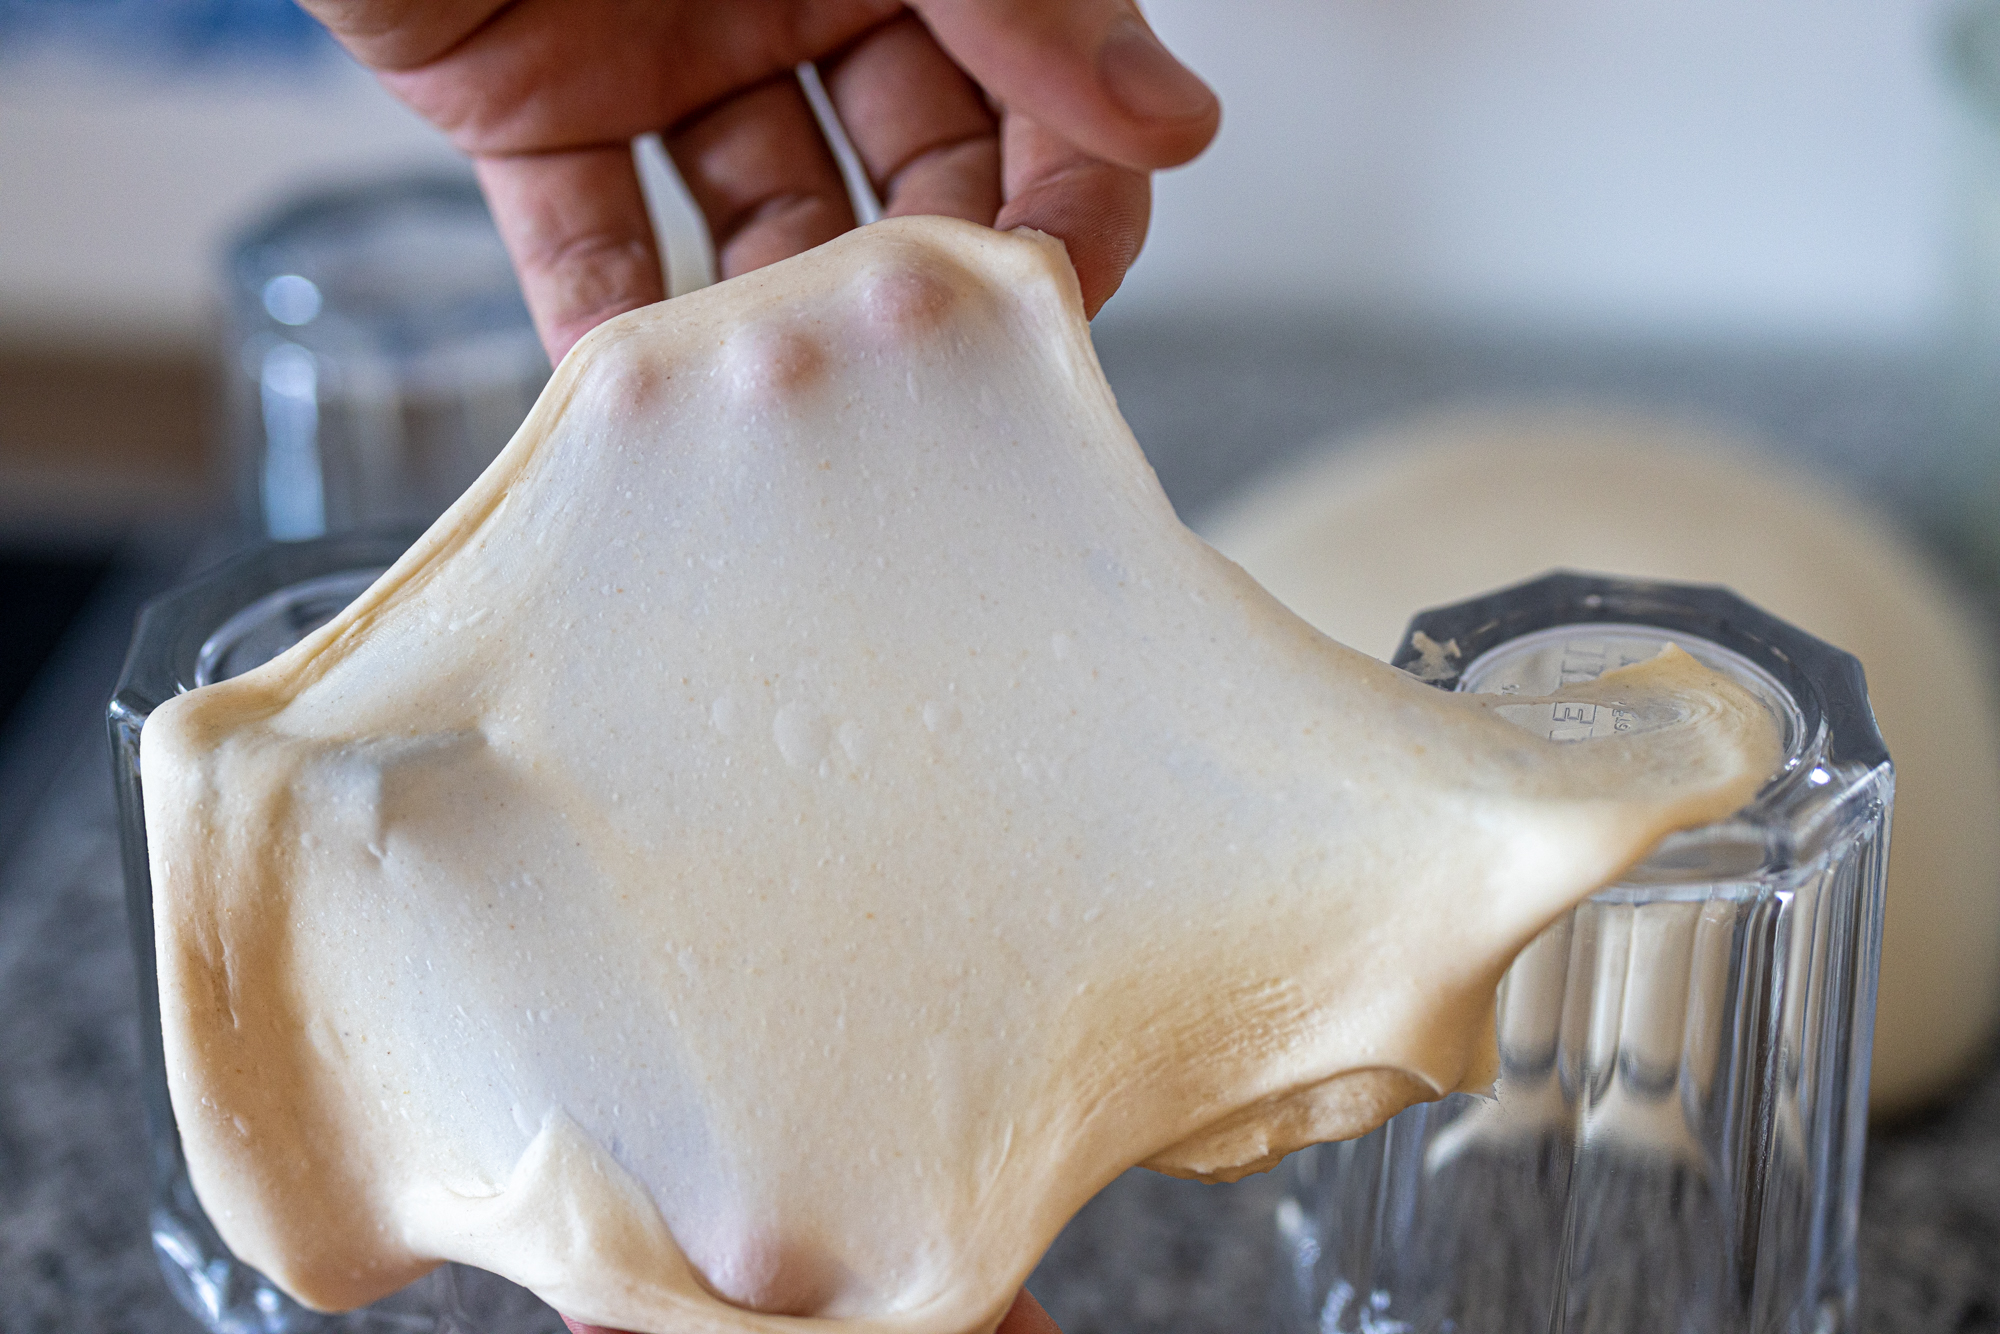
\includegraphics[width=\textwidth]{window-pane-effect}
  \caption[The window pane test]{The window pane test allows you to see if you
      developed your gluten well enough.}
\end{figure}


From an economic perspective, water is the cheapest component in your bread
dough. When running a bakery, a higher hydrated dough will weigh more and have
lower production costs. The profit will be higher. This comes at the price
of increasing labor costs and more potential failures due to the enhanced
difficulty.

\section{How much starter?}

Most bakers use around \qty{20}{\percent} sourdough starter based on the
flour weight.  I~recommend going much lower, to around
\qtyrange{5}{10}{\percent}.

By adjusting the amount of pre-ferment you can influence the time your dough
requires in the bulk fermentation stage. The more starter you use, the faster
this process is. The smaller the starter quantity, the slower. With a higher
quantity of starter, you are introducing more microorganisms to your main
dough. The higher this quantity, the faster the rate of fermentation in your
dough is.

The other factor influencing the rate of fermentation is the temperature of
your dough. The warmer the temperature, the faster the process; the colder, the
slower the process.

While food is available, the microorganisms will reproduce and increase in
quantity. The process is self-limiting: it stops when there is no
more food available. This can be compared to wine making where
the yeast ultimately sporulates and dies as ethanol levels increase. The ethanol creates an
environment that makes it impossible for other
microorganisms to join the feast. The same thing happens with the acidity
created by the bacteria. The high acidity slows the fermentation process and
prevents new microorganisms from entering the system.

Initially, your starter's properties are carried over to the main dough. Then,
as time progresses, the microorganisms adapt to the new environment. If your
starter is very bacterial then your main dough's fermentation will also be. You
end up with a dough that is not as fluffy as it could be. It will taste quite
sour, too sour for most people.

If you were to use an extreme value of around \qty{90}{\percent} starter based on your flour, there
would be very little room for the microorganisms to adjust in the main dough.
If you were to just use \qty{1}{\percent}, your microorganisms can regrow into a
desirable balance in the dough. Furthermore, you need to consider that a high value
of starter means a high inoculation with already fermented flour. As
mentioned earlier, enzymes break down the dough. This means the higher this
value, the more broken-down fermented flour you have. A too-long fermentation
always results in a very sticky dough that cannot be handled. The more
starter you use, the faster you will get to this point. If you were to use a
very little amount of starter, your flour might have naturally broken down
before the fermentation has reached the desired stage. You can observe this
when using a small quantity of around \qty{1}{\percent} sourdough starter. The small
amount of added microorganisms will not be able to reproduce fast enough
before the protease has broken down your dough completely.

As explained earlier the key to making great bread is a slow but not too slow
fermentation. Enzymes require time to break down your dough. Taking all this
into consideration, I~try to aim for a fermentation time of around 8 to 12~hours. This seems to be
the sweet spot for most of the flours that I~have worked with. To achieve this,
I~use around \qty{5}{\percent} of sourdough starter in summer times
(temperatures around \qty{25}{\degreeCelsius} (\qty{77}{\degF}) in the
kitchen). In winter times I~opt for around \qty{10}{\percent} up to
\qty{20}{\percent} sourdough starter (kitchen temperature around
\qty{20}{\degreeCelsius} (\qty{68}{\degF})). This
allows me to use a sourdough starter that's not in perfect condition. As
explained earlier, your
bread dough is essentially a gigantic starter. The low inoculation rate allows
the starter to regrow inside your main dough into a desirable balance.
Furthermore, the enzymes have enough time to break down the flour. This also
allows me to skip the so-called autolysis step completely (more in the next section).
This greatly simplifies the whole process.

\section{Autolysis}%
\label{section:autolysis}

Autolysis describes the process of just mixing flour and water and letting
this sit for a period of around 30~minutes up to several hours. After this
process is completed, the sourdough starter and salt are added to the
dough\footnote{I~have tested adding the salt at the start and end of the
autolysis process and could not notice a difference. Based on my current
understanding, the importance of adding salt later seems to be a myth.}.

The overall time that flour and water are in contact is extended. Thus you get the
beneficial enzymatic reactions that improve the taste and characteristics of the
dough. I~do not recommend autolysis as it adds an unnecessary step to the
process. Instead, I~recommend the fermentolysis technique which will be covered in the
next section of this book.

The effects of autolysis are very interesting. Try to mix just flour and
water and let that sit for a day. During the day, check the consistency of
your dough. Try and stretch the dough. If you dare, you can also taste the
dough throughout the day. With each hour, your dough will become
more extensible. It will be easier to stretch the dough. At the same time, your
dough will start to taste sweeter and sweeter. The protease and amylase enzymes
are doing their job. The same process is used when making oat milk. By letting
the mixture sit for some time, enzymes work on the oats. The taste is perceived as
sweeter and more appreciated. This process is further accelerated the more
whole-grain your flour is. The hull contains more enzymes. The gluten network
will ultimately tear, and your dough flattens out. For wheat sourdough, this is
your worst enemy. When this happens, your dough will become leaky and release
all that precious gas created during the fermentation. You need to find the
right balance of your dough breaking down just enough and not too much.

When you use a high inoculation rate of around \qty{20}{\percent} sourdough starter
your fermentation can be very quick. At \qty{25}{\degreeCelsius} it could be finished in as little as 5~hours.
If you ferment longer, your dough becomes leaky. At the same time, in
these 5~hours, the enzymes have not broken down the flour enough. This means
the dough might not be as elastic as it should be. Furthermore, not enough
sugars have been released and thus the flavor after baking is not good
enough\footnote{I~have not seen studies yet looking at enzymatic speeds depending on
the temperature. But I~assume the higher the temperature, the faster these
reactions. This goes up until a point when the enzymes break down under
heat.}. That's why bakers opt for autolysis. The autolysis starts the enzymatic
reactions before the microorganism fermentation begins. This way after 2~hours
of autolysis (an example) and 5~hours of fermentation the dough is in the
perfect state before beginning proofing.

When you try to mix your salt and starter into the flour/water dough you will
notice how cumbersome this is. It feels like you have to knead again from scratch
one more time. You will spend more time mixing dough.

For that reason, I~am strongly advocating utilizing the fermentolysis approach
which greatly simplifies the mixing and kneading process.

\section{Fermentolysis}%
\label{section:fermentolysis}

The fermentolysis creates the same advantageous dough properties the
autolysis creates without the headache of mixing your dough twice. You do this
by extending the fermentation time of your dough. Rather than doing a 2-hour
autolysis and 5-hour bulk fermentation you opt for an overall 7-hour
fermentation period.

To do this, you use less sourdough starter. A conventional recipe including the
autolysis step might call for \qty{20}{\percent} sourdough starter. Simply reduce this
value to \qtyrange{5}{10}{\percent}. The other option could be to place the dough in a colder
environment and thus reduce the speed at which your microorganisms replicate.

\begin{table}[!htb]
    \centering
        \documentclass[tikz]{standalone}
\usepackage{tikz}
\usepackage{siunitx}
\DeclareSIUnit\degF{\text{°}F}

\begin{document}
\begin{tabular}{|l|l|l|l|}
\hline
\textbf{\begin{tabular}[c]{@{}l@{}}Temperature\\ in °C\end{tabular}} & \textbf{\begin{tabular}[c]{@{}l@{}}Temperature\\ in °F\end{tabular}} & \textbf{\begin{tabular}[c]{@{}l@{}}Starter\\ recently fed?\end{tabular}} & \textbf{\begin{tabular}[c]{@{}l@{}}Amount\\ of starter in\%\end{tabular}} \\ \hline
30                                                                   & 86                                                                   & Yes                                                                      & 5                                                                         \\ \hline
25                                                                   & 77                                                                   & Yes                                                                      & 10                                                                        \\ \hline
20                                                                   & 68                                                                   & Yes                                                                      & 15                                                                        \\ \hline
30                                                                   & 86                                                                   & No                                                                       & 2.5                                                                       \\ \hline
25                                                                   & 77                                                                   & No                                                                       & 5                                                                         \\ \hline
20                                                                   & 68                                                                   & No                                                                       & 10                                                                        \\ \hline
\end{tabular}
\end{document}

        \caption[Quantity of sourdough]{A table visualizing how much sourdough
            starter to use depending on temperature and the starter's activity
            level.}
\end{table}

Based on my experience and my sourdough, my ideal bread always takes around 8
to 12~hours during bulk fermentation. Based on my availability throughout
the day, I~use a higher or lower starter quantity. If I~wanted to achieve a completed
fermentation in 8~hours, I~would opt for a \qty{10}{\percent} sourdough starter. If
I~wanted it to be ready in 12~hours, I~would opt for less starter, around \qty{5}{\percent}.
Simply mix all the ingredients and your fermentation begins. The
enzymes and microorganisms commence their work. On a very warm summer day, the
mentioned quantities no longer work. With a \qty{10}{\percent} starter, the same dough
would be ready in 5~hours up to a point of no return. Another additional hour
would cause the dough to break down too much. In this case, I~would opt for 5
percent sourdough starter to slow the whole process down to reach the 8 to 12
hour window again. If it is very hot, I~might use as little as \qty{1}{\percent}
sourdough starter\footnote{Please take these values with a grain of salt as
they depend on your flour and your sourdough starter. These are values that
you have to experiment with. After baking a couple of breads you will be able
to read your dough much better.}. You have to play with the timings on your own.
Rather than relying on timing though, I~will show you a much better and more precise approach
by using a fermentation sample. This will be covered later in this chapter.

Even for yeasted doughs, I~no longer use autolysis. I~just reduce the amount
of yeast that I~am using. Opting for the fermentolysis will
save you time and simplify your bread-making process. As mentioned in previous chapters,
the secret to making great bread is a slow but not too slow fermentation.

\section{Dough strength}

Dough strength is a fancy way to describe the bread-kneading process. As you wait and
knead, the gluten bonds in your dough become stronger. The dough
becomes more elastic and holds together better. This is the basis for trapping
all the gases during the fermentation process. Without the gluten network,
the gases would just diffuse out of your dough.

\begin{flowchart}[!htb]
\centering
  \begin{tikzpicture}[node distance = 3cm, auto]
  \node [start] (init) {\footnotesize Homogenize recipe ingredients};
  \node [block, right of=init, node distance=3cm] (wait1) {\footnotesize Wait 15~minutes};
  \path [line] (init) -- (wait1);
  \node [block, right of=wait1, node distance=3cm] (knead1) {\footnotesize Knead 5~minutes};
  \path [line] (wait1) -- (knead1);
  \node [block, right of=knead1, node distance=3cm] (wait2) {\footnotesize Wait 15~minutes};
  \path [line] (knead1) -- (wait2);
  \node [decision, below of=wait2, node distance=3cm] (windowpane_test) {\footnotesize Window-pane?};
  \path [line] (wait2) -- (windowpane_test);
  \path [line] (windowpane_test) -- node{no} (knead1);
  \node [decision, left of=windowpane_test, node distance=4.5cm] (more_water) {\footnotesize Bassinage for more water?};
  \path [line] (windowpane_test) -- node{yes} (more_water);
  \node [block, left of=more_water, node distance=4.5cm] (add_water) {\footnotesize Add water};
  \path [line] (more_water) -- node{yes} (add_water);
  \path [line] (add_water) -- (knead1);
  \node [block, below of=add_water, node distance=4cm] (wait3) {\footnotesize Wait 15~minutes};
  \path [line] (add_water) -- (wait3);
  \node [decision, right of=wait3, node distance=4.5cm] (dough_sample) {\footnotesize Aliquot sample?};
  \path [line] (wait3) -- (dough_sample);
  \path [line] (more_water) -- node{no} (dough_sample);
  \node [block, right of=dough_sample, node distance=4.5cm] (dough_ball) {\footnotesize Make round dough ball};
  \path [line] (dough_sample) -- node{no} (dough_ball);
  \node [block, below of=dough_sample, node distance=3cm] (extract_sample) {\footnotesize Extract sample};
  \path [line] (dough_sample) -- node{yes} (extract_sample);
  \path [line] (extract_sample) -- (dough_ball);
  \node [success, below of=dough_ball, node distance=3cm] (begin_bulk) {\footnotesize Begin bulk fermentation};
  \path [line] (dough_ball) -- (begin_bulk);
\end{tikzpicture}

  \caption{The gluten development process for a wheat-based dough.}%
  \label{fig:wheat-sourdough-kneading-process}
\end{flowchart}

It might sound odd, but the most important part of kneading is waiting. By
waiting you are allowing your flour to soak up water. This way the gluten
bonds of your dough form automatically and your dough becomes more elastic.
So you could be kneading for 10~minutes initially just to be surprised
that kneading 5~minutes and waiting 15~minutes has the same effect.

The gluten proteins glutenin and gliadin virtually instantly bond after being
hydrated. Disulfide bonds enable the longer portions of
glutenin to join with one another and form sturdy, extensible molecules.
Glutenins add strength, whilst the more compact gliadin proteins allow
the dough to flow like a fluid. Ultimately, the longer you wait, the more
your gluten network transforms into a web-like structure. This is what
traps the gases during the fermentation process~\cite{how+does+gluten+work}.

\begin{figure}[!htb]
  \centering
  \begin{tikzpicture}
    \tikzstyle{every node}+=[font=\normalsize\rmfamily]
    \begin{axis}[
        title style={align=center},
        title={Gluten development of a sourdough and yeast based dough\\
                \qty{22}{\degreeCelsius} (\qty{72}{\degF}) and
                \qty{60}{\percent}~hydration},
        axis x line=middle,
        axis y line=middle,
        width=\textwidth,
        height=0.5\textwidth,
        xmax=44, xmin=-0.1,
        ymax=12, ymin=-0.1,
        every axis y label/.style={%
            at={(ticklabel cs:0.5)},rotate=90,anchor=near ticklabel}, 
        every axis x label/.style={%
            at={(ticklabel cs:0.5)},anchor=near ticklabel}, 
        xtick distance=6,
        ytick style={draw=none},
        yticklabels={empty},
        legend style={draw=none},
        legend cell align={left},
        xlabel=Duration (hours), ylabel=Dough strength
        ]
        \addplot [color=redpic,smooth,ultra thick] table {plots/yeast.table};
        \addplot [color=codeblue,smooth,ultra thick] table {plots/sourdough.table};

        \node at (axis cs:18,7) [anchor=south west] {%
            \begin{tabular}{@{}lll@{}} \textbf{Dough type}&
            \textbf{Kneading} & \textbf{Stretch \& Fold}\\
            \midrule
            \textcolor{redpic}{Yeast}  & \textcolor{redpic}{None}&
            \textcolor{redpic}{None}  \\ \textcolor{codeblue}{Sourdough}&
            \textcolor{codeblue}{None} & \textcolor{codeblue}{None} \\
            \end{tabular}
        };
        \node at (axis cs:8,8.3) [anchor=south] {Peak stage};
        \node at (axis cs:1,1) [anchor=west] {Development stage};
        \node at (axis cs:9.5,5) [anchor=west] {Extensibility stage};
        \node at (axis cs:25.8,4) [anchor=west] {Decay stage};
    \end{axis}
\end{tikzpicture}

  \caption[Dough strength over time without kneading]{A schematic
      visualization of automatic gluten development. The doughs are not
      kneaded, just initially mixed.  Note how dough strength deteriorates
      over time as enzymes break down the flour. The effect is accelerated for
      sourdough due to the bacteria's gluten proteolysis.}%
  \label{fig:wheat-yeast-sourdough-degradation}
\end{figure}

The soaking process has to be extended the more whole-wheat flour is used.
The purpose of the wheat kernel's outer bran is to soak up water as fast
as possible. The enzymes become activated and start the sprouting process.
Because of this, less water is available for the gluten bonds to develop.
Either wait a bit longer or proceed and use slightly more water for
the dough.

This is the same principle that popular no-knead recipes follow. By making a less
hydrated dough and waiting your gluten network automatically forms. You still
have to mix and homogenize the ingredients. You wait a few minutes just to
find your dough having developed incredible dough strength with no additional
kneading\footnote{Give it a shot yourself. The automatic formation of gluten
networks is an amazing phenomenon that still fascinates me every time I~am
making dough.}.

If you over-hydrate your dough at the beginning it becomes more difficult
for the gluten chains to form. The molecules are not as close together in
a wetter dough compared to a stiffer dough. It is harder for the molecules
to align and form the web structure. For this reason, it is always easier
to start with lower hydration and then increase the water quantity if needed.
This is also commonly known as the \emph{Bassinage method}. The gluten
bonds have formed at the lower hydration and can then be made more extensible
by adding water and kneading again. This is a great trick to make
a more extensible dough with lower-gluten flour~\cite{bassinage+technique}.

When machine kneading a dough, opt for the same technique shown in
Flowchart~\ref{fig:wheat-sourdough-kneading-process}.  Initially opt for a low
speed. This helps the homogenization process.
After waiting to allow the flour to soak up the water, proceed on a higher speed
setting. A good sign of a well-developed gluten network is
that your dough lets go of the container. This is because of the gluten's elasticity.
The elasticity is higher than the desire of the
dough to stick to the container.

\begin{figure}[!htb]
  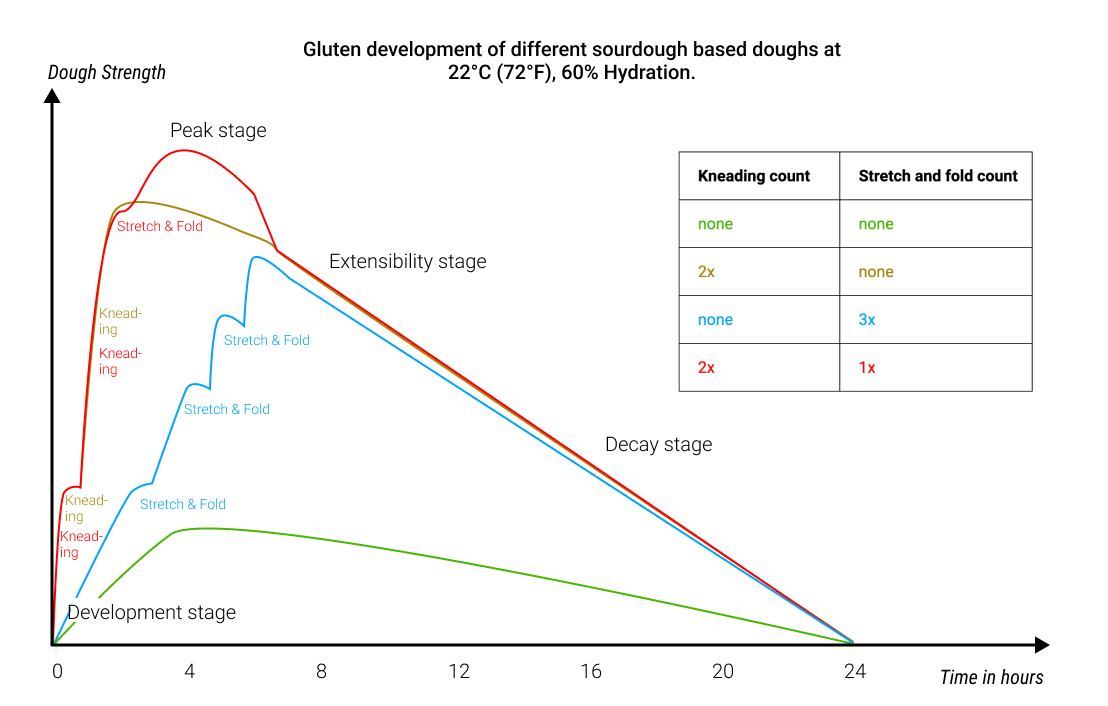
\includegraphics[width=\textwidth]{dough-strength-sourdough}
  \caption[Dough strength over time with kneading]{A schematic visualization
      of gluten development in sourdoughs with different kneading techniques.
      A combination of techniques can be utilized to achieve maximum dough
      strength.}%
  \label{fig:dough-strength-sourdough}
\end{figure}
% See https://www.figma.com/file/wTUVe6Nm2INOvT82mJhQur/Dough-strength-visualisation?node-id=0%3A1&t=fjdPvXYuJpsdQfWN-1 for
% the source of this visualization

Generally, the more dough strength you create, the less sticky your dough is going to
feel. As the dough holds together, it will no longer stick to your hands as
much. This is a common problem beginners face. Sticky dough is frequently
the sign of a not well enough developed gluten network.

\begin{figure}[!htb]
  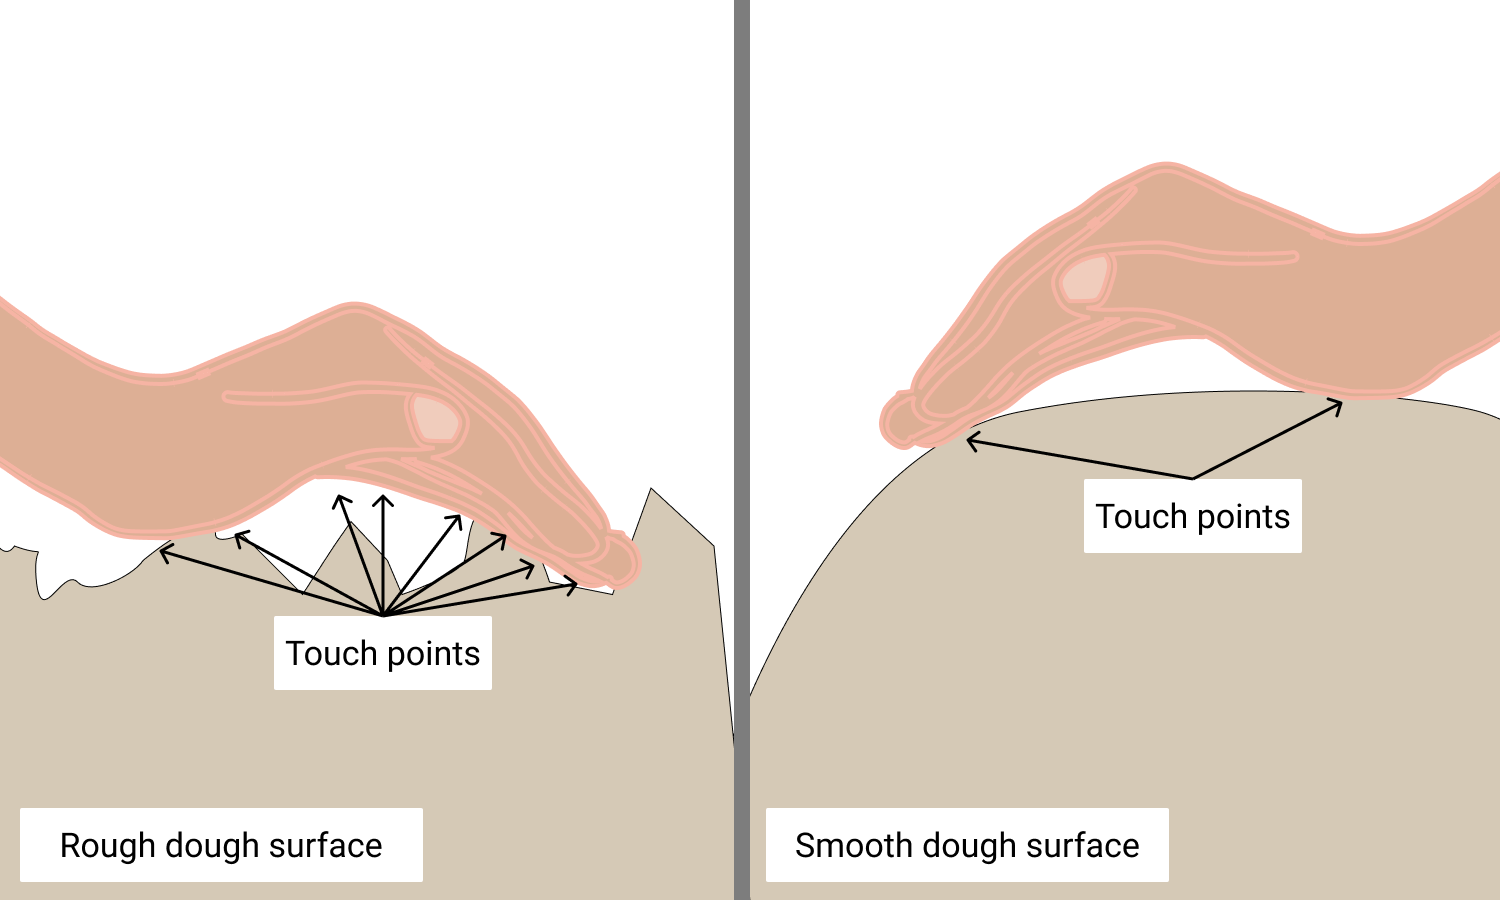
\includegraphics[width=\textwidth]{dough-surface-touchpoints}
  \caption[Touching the dough surface]{A schematic visualization of how a rough
      dough surface creates more touch points compared to a smooth dough
      surface.  By touching the rough surface the dough will swell and get into
      contact with more areas of your hand.}%
  \label{fig:dough-touch-points}
\end{figure}

Kneading more is generally beneficial in almost all cases, as it results in a
stronger gluten network. However, when making soft milk breads, you might prefer
a more extensible dough from the start. In this scenario, excessive kneading
could lead to a chewier final bread, which is not desirable if you aim for a
fluffier texture. Achieving this fluffier dough can be accomplished by kneading
less. While this is an exception, properly kneading your wheat-based doughs
is generally advised.

When you use a stand mixer, you can run into the issue of kneading too much. This
is almost impossible in practice though. Even after kneading for 30~minutes on medium
speed, my doughs hardly ever were over-kneaded. The moment you knead
too much, the color of the dough can begin to change. You mostly
notice this, though, during baking. The resulting loaf looks very
pale and white. This is because mixing dough causes oxidation,
which is necessary for the development of gluten.
However, if the dough is mixed too much, the compounds that contribute
to the bread's flavor, aroma, and color may be destroyed, negatively
affecting the quality of the bread~\cite{oxidization+dough}.

The last step before beginning bulk fermentation is to
create a smooth dough ball. By making sure your dough's surface is
smooth, you will have fewer touch points when touching the dough.
See Figure~\ref{fig:dough-touch-points} for a schematic visualization
of how your hand touches a rugged and smooth dough.
With the smooth surface, your dough is going to stick less on your hands. Applying
later stretches and folds will be a lot easier. Without a smooth
surface, the dough becomes almost unworkable. Folding the dough later
becomes an impossible task. This is a frequent mistake I~see many
new bakers commit.

\begin{figure}[!htb]
  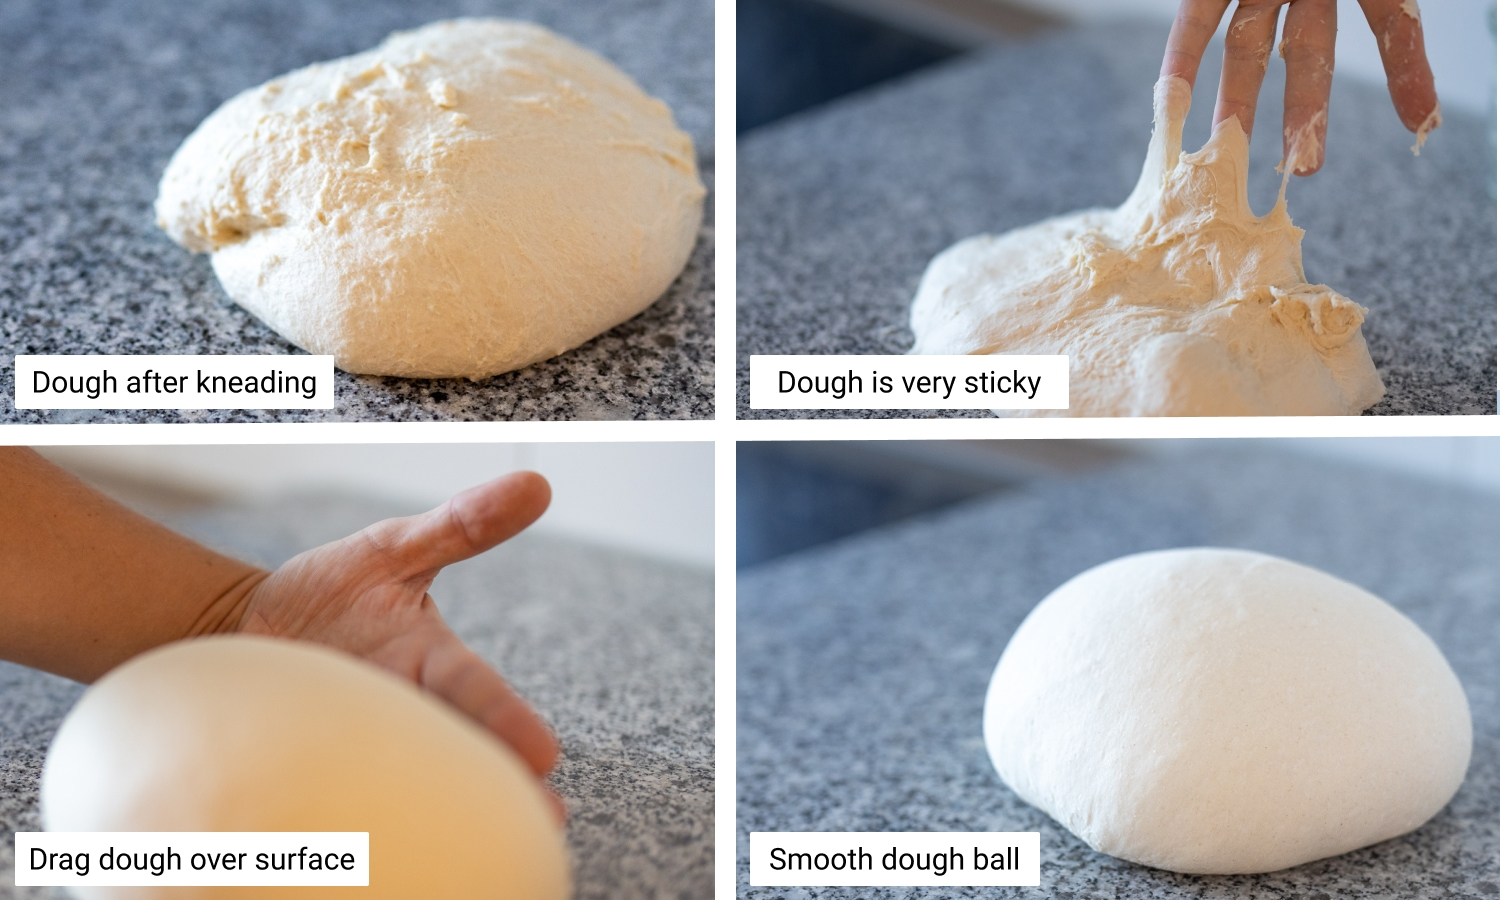
\includegraphics[width=\textwidth]{dough-ball-steps}
  \caption[Creating a smooth surface]{The transformation of a sticky dough
      blob to a dough with a smooth surface. The goal is to reduce surface
      touchpoints with your hands to make the dough less sticky when working
      it.}%
  \label{fig:dough-ball-steps}
\end{figure}

To make the dough's surface smooth, place your dough on a wooden board or
on your kitchen's countertop. Drag the dough with your palm over the surface.
A dough scraper could be used here for assistance.
Drag the dough towards you while making sure the top center of the dough stays in place.
It can help to gently place your second hand on top of the dough so that
the dough mass moves while retaining its orientation. Once the whole dough
is too close to the edge of the container/countertop, gently move it back
with two hands. By doing so, you are stretching the outer surrounding gluten layer.
For this reason, it is important to not use any flour during this process.
By using flour, you can no longer drag the dough over the surface and thus
you can't stretch the gluten. Always imagine you are touching something utterly sticky.
By doing so you will automatically try to touch the dough as little
as possible. Keep repeating the process until you see that the dough
has a nice smooth surface. The final dough should look like the dough
shown in Figure~\ref{fig:dough-ball-steps}.

If your outer gluten layer tears, you have overstretched your dough. In
that case, take a 10-minute break, leaving your dough on the kitchen countertop.
This allows the gluten to re-bond and heal. Repeat the same process
and the damaged rugged areas should disappear.

The same dough-rounding technique is used later during
the pre-shaping process. After creating dough strength you
have all the time you need to practice rounding. Round the dough
as much as possible until it tears. Then wait the aforementioned 10~minutes and repeat.
Later, you don't have any room for error. Your technique has to be on point.
An over-pre-shaped dough can potentially not recover.

\section{Bulk fermentation}%
\label{section:bulk-fermentation}

After mixing the starter into your dough, the next stage of
the process known as bulk fermentation begins. The term
\emph{bulk} is used because in bakeries, multiple loaves are fermented
together in bulk. If you are a home baker, you might bulk
ferment a single loaf. The bulk fermentation ends when you
divide and pre-shape, or directly shape your final loaves or loaf.

The hardest part when making sourdough bread is controlling
the fermentation process. Bulking long enough but not too
long is the deciding factor for making great bread at home.
Even with poor shaping and baking techniques, you'll be able
to make excellent bread, solely by mastering the bulk
fermentation process.

With a too-short bulk, your crumb will be
perceived as gummy. Your crumb will feature large pockets of
air commonly referred to as \emph{craters}. A too-long fermentation
results in the dough breaking down too much. The resulting
dough will stick to your banneton and spread while baking
into a pancake-like structure.

The key is to find the sweet spot between not too little
and not too much bulk fermentation. I'd always recommend pushing
the dough more toward a longer fermentation. The
flavor of the resulting bread is better compared to a pale
underfermented dough.

\begin{table}[!htb]
    \centering
        \begin{tabular}{@{}>{\bfseries}p{0.12\textwidth}p{0.273\textwidth}p{0.273\textwidth}p{0.273\textwidth}@{}}
\toprule
 &\multicolumn{3}{c}{\textbf{Fermentation}}\\
 \cmidrule(rl){2-4}
 & \thead{Too short} & \thead{Too long} & \thead{Perfect} \\ \midrule
Crumb texture & Unbaked gummy areas towards the bottom of the bread.
              & Crumb can be perceived as gummy as most gluten broken down.
              & Crumb evenly baked. Crumb can be perceived as moist, but not gummy.
              \\ 
Alveoli       & Overly large alveoli in the crumb ``craters''.
              & Many tiny alveoli equally distributed.
              & Alveoli evenly distributed, no ``craters''.
              \\ 
Taste         & Pale neutral taste.
              & Strong acidic flavor profile. Acidity overweighs when tasting.
              & Balanced flavor profile, not too mild but also not too sour.
              Depending on starter vinegary or lactic notes.
              \\ 
Texture       & Overall poor texture.
              & Good consistency, crumb is not as fluffy as it could be.
              & Great combination of  textures.
              \\ 
Oven spring   & Vertical oven spring, mostly due to water evaporating and inflating the dough.
              & Very flat pancake like  structure after baking.
              & Great vertical oven spring. Dough grows more upwards rather than sideways.
              \\ \bottomrule
\end{tabular}

        \caption[Stages of sourdough fermentation]{The different stages of
            sourdough fermentation and the effects on crumb, alveoli, texture,
            and overall taste.}
\end{table}

The worst thing you can do when fermenting sourdough
is to rely on a recipe's timing suggestions. In \qty{99}{\percent}
of the cases, the timing will not work for you. The writer
of the recipe probably has different flour and a different
sourdough starter with different levels of activity. Furthermore,
the temperature of the fermentation environment might be
different. Just small changes in one parameter result
in a completely different timing schedule. One or two~hours'
difference results in the dough not fermenting long enough, or
turning it into a gigantic sticky fermented pancake. This
is one of the reasons why the current baking industry prefers
to make solely yeast-based doughs. By removing the bacteria
from the fermentation, the whole process becomes a lot more
predictable. The room for error (as shown in
Figure~\ref{fig:wheat-yeast-sourdough-degradation}) is much larger. The doughs
are perfect to be made in a machine.

\begin{flowchart}[!htb]
\centering
  \begin{tikzpicture}[node distance = 3cm, auto]
  \node [start] (init) {Bulk fermentation};
  \node [block, right of=init, node distance=4cm] (check_dough) {Check the dough};
  \node [block, right of=check_dough, node distance=4cm] (size_increase) {Check dough size increase};
  \node [block, below of=size_increase, node distance=2cm] (ph_value) {Check dough pH value};
  \node [block, below of=ph_value, node distance=2cm] (smell) {Check dough smell};
  \node [decision, right of=size_increase, node distance=4cm] (dough_ready) {Dough ready?};
  \node [success] at(dough_ready |- smell) (divide_preshape) {Divide and preshape};
  \node [decision, above of=size_increase] (dough_flattened) {Dough flattened out?};
  \node [block, above of=check_dough] (wait_60_minutes) {Wait\\ 60~minutes};
  \node [block, above of=wait_60_minutes] (stretch_fold) {Stretch and fold};

  \path [line] (init) -- (check_dough);
  \path [line] (check_dough) -- (size_increase);
  % Tricks not to get double lines
  \path [line] (check_dough) ++(2, -2) -- node{or} (ph_value);
  \path [line] (check_dough) ++(2, 0) -- node{} ++(0, -4) -- node{or} (smell);
  \path [line] (check_dough) ++(2, -4) -- node{or} (smell);
  \path [line] (size_increase) -- (dough_ready);
  % Same tricks not to get double lines and also we do _not_ want arrows
  \path [draw, thick] (ph_value) -- node{} ++(2, 0);
  \path [draw, thick] (smell) -| node{} ++(2, 4);
  \path [line] (dough_ready) -- node{Yes} (divide_preshape);
  \path [line] (dough_ready) |- node[right=3pt]{no} (dough_flattened);
  \path [line] (dough_flattened) |- node[right=3pt]{yes} (stretch_fold);
  \path [line] (dough_flattened) -- node{No} (wait_60_minutes);
  \path [line] (stretch_fold) -- (wait_60_minutes);
  \path [line] (wait_60_minutes) -- (check_dough);
\end{tikzpicture}

  \caption[Process to check the bulk fermentation]{During the bulk
      fermentation, multiple doughs are fermented together in bulk.  A
      challenging aspect of homemade sourdough bread is to determine when this
      stage of fermentation is completed. This chart shows multiple available
      options to check on the bulk fermentation progress.}%
  \label{fig:bulk-fermentation}
\end{flowchart}

Experienced bakers will tell you to go by the look and feel of
the dough. While this works if you have made hundreds of loaves,
this is not an option for an inexperienced baker. As
you make more and more dough, you will be able to judge
the dough's state by touching it.

My go-to method for beginners is to use an \emph{Aliquot jar}.
The aliquot is a sample that you extract from your dough. The
sample is extracted after creating the initial dough strength.
You monitor the aliquot's size increase to judge the
level of fermentation of your main dough. As your
dough ferments, so does the content of your aliquot jar. The moment your
sample reached a certain size, your main dough is ready
to be shaped and proofed. The size increase you should
aim for depends on the flour you have at hand. A flour
with a higher gluten content can be fermented for a
longer period. Generally, around \qty{80}{\percent}
of your wheat flour's protein is gluten. Check your flour's
packaging to see the protein percentage. The actual size increase
value is highly variable depending on your flour composition.
I~recommend beginning with a size increase of \qty{25}{\percent} and testing
up to \qty{100}{\percent} with subsequent bakes. Then identify a value
that you are happy with.

\begin{table}[!htb]
    \centering
        %TODO: Not great looking
\begin{tabular}{@{}cc@{}}
\toprule
\thead{Flour protein content} & \thead{Relative aliquot size increase} \\ \midrule
8--10\%              & 25\%  \\ 
10--12\%             & 50\%  \\ 
12--15\%             & 100\% \\ 
\textgreater{} 15\%  & \textgreater{} 100\% \\ \bottomrule
\end{tabular}

        \caption[Increase of size versus protein content]{Reference values for
            how much size increase to aim for with an aliquot jar depending on
            the dough's protein content.}
\end{table}

The beauty of the aliquot is that no matter the surrounding
temperature, you will always know when your dough is ready.
While the dough might be ready in 8~hours in summer, it could
easily be 12~hours in winter. You will always ferment your
dough exactly on point.


\begin{figure}[!htb]
  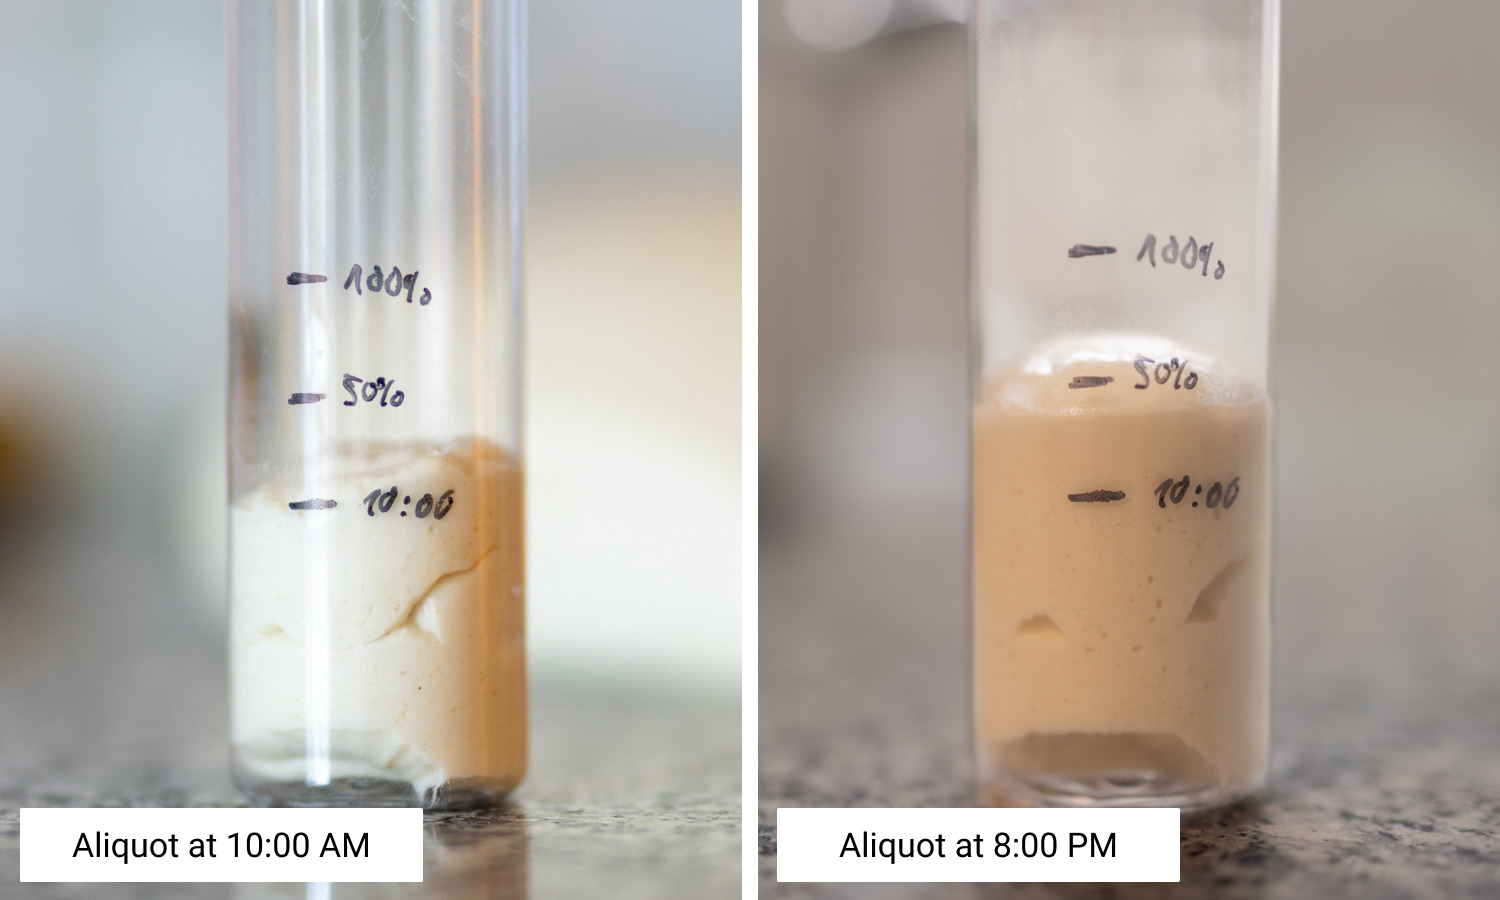
\includegraphics[width=\textwidth]{aliquot-before-after}
  \caption[Aliquot Jar]{An aliquot jar to monitor the dough's fermentation
      progress.  It took 10~hours for the dough to reach a \qty{50}{\percent}
      size increase.}
\end{figure}

While the aliquot sample has enabled me to consistently bake
great loaves, there are limitations to consider. It's crucial
to use a cylindrical-shaped container to properly judge
the dough's size increase. Furthermore, it is essential
to use room-temperature water when making your dough. If the
water is hotter, your aliquot, due to its smaller size,
will cool down faster. The aliquot will ferment more slowly
than your dough. Similarly, when you use too cold water,
your sample will heat up faster than the large dough mass.
In that case, your aliquot is ahead of your main dough. You
would probably stop the fermentation too early. Make sure
to keep the dough and aliquot close together. Some people even
place the aliquot in the same container. This makes sure that
both are in the same environment temperature. The aliquot
is also less reliable if your ambient temperature changes
a lot during the day. In that case, your aliquot will adapt
faster than your main dough. The readings will always be slightly
off. If you are making a large chunk of dough with more
than \qty{10}{\kg} of flour, the jar is also less reliable. The biochemical
reactions happening inside your dough will heat it.
The fermentation itself is exothermic which means
that it produces heat.

Another more expensive option is to use a pH meter
to monitor your dough's fermentation state. As the lactic
and acetic acid bacteria ferment, more acidity is piled
up inside your dough. The acidity value (pH) can be
measured using such a meter. The more acidity, the lower the pH
value of your dough. The pH scale is logarithmic, meaning
that each digit change will have a 10x increase in acidity.
A sourdough dough might begin fermenting at \pHvalue{6.0},
then shortly before baking has roughly \pHvalue{4.0}. This means
that the dough itself is 10x times 10x (= 100x) sourer
than at the beginning. By using the meter, you can always
judge the state of your dough's acidification and then act
accordingly.

To use the pH meter successfully, you need to find pH values
that work for your dough. Depending on your starter,
water, and flour composition, the pH values to look out
for are different. A stronger flour with more gluten
can be fermented for a longer period. To find out
the pH values for your bread I~recommend taking
several measurements while making your dough.

\begin{enumerate}
  \item Measure the pH value of your sourdough starter before using it
  \item Check the pH after mixing all the ingredients
  \item Check the pH before dividing and pre-shaping
  \item Check the pH before shaping
  \item Check the pH of your dough before and after proofing
  \item Check the pH of your bread after baking
\end{enumerate}

If the bread you made turned out successfully with your values,
you can use them as a reference for your next batch. If the
bread didn't turn out the way you like, either shorten
the fermentation or extend it a little bit.

\begin{table}[!htb]
    \centering
        \begin{tabular}{@{}lr@{}}
\toprule
\textbf{Step}       & {\textbf{pH Value}} \\ \midrule
Starter ready       & 4.20                \\ 
Mixing              & 6.00                \\ 
Dividing/preshaping & 4.10                \\ 
Shaping             & 4.05                \\ 
Before proofing     & 4.03                \\ 
After proofing      & 3.80                \\ 
After baking        & 3.90                \\ \bottomrule
\end{tabular}
%
        \caption[Dough's pH during bread preparation]{Example pH values for
            the different breakpoints of my own sourdough process.}%
        \label{table:sample-ph-values}
\end{table}

The beauty of this method is its reliability. Once you have found
out your good working values, you can reproduce
the same level of fermentation with each subsequent dough.
This is especially handy for large-scale bakeries that want
to achieve consistency in each bread.

While this method is very reliable, there are also certain
limitations to consider.

First of all the pH values that work for me likely won't work for
you. Depending on your own starter's composition of lactic
and acetic acid bacteria, your pH values will be different.
You can use the values shown in Table~\ref{table:sample-ph-values}
as rough ballpark figures. Regardless, you need to find values
that work for your setup.

Another limitation is the price. You will need to purchase
a high-tech pH meter, ideally, a meter featuring a spearhead
\footnote{Not every pH meter is suitable for measuring dough.
Please refer to the manual to make sure it is certified for
measuring the pH of liquid and semi-solid media. To receive
accurate pH readings further ensure that your pH meter
is properly calibrated.}.
This way you can directly poke the meter deep into the dough.
At the same time, automated temperature adjustments are a
feature to look out for. Depending on the temperature,
the pH value varies. There are tables you can use to
do the adjustment calculations. More expensive meters
have this feature built in. The pH meter loses accuracy
over time. For this reason, you need to frequently
calibrate it. The process is cumbersome and takes time.
Lastly, you need to carefully rinse the pH meter before
using it in your dough. The liquid surrounding the
head of your pH meter is not food-safe and thus should
not be eaten. I~rinse the meter for at least one minute
before using it to measure my dough's fermentation stage.

The last method to judge the state of bulk fermentation
is to read the signs of your dough. The more bread you have
made, the more accustomed you will become to this process.
Look out for the dough's size increase. This can sometimes
be a challenge when your dough is inside a container.
You can help yourself by marking your container. Some bakers
even use a transparent rectangular bulk container. You
can use a pen to mark the initial starting point. From there
on you can nicely observe the size increase. Similar to the
mentioned aliquot sample, look out for a size increase that works
for your sourdough composition.

\begin{figure}[!htb]
  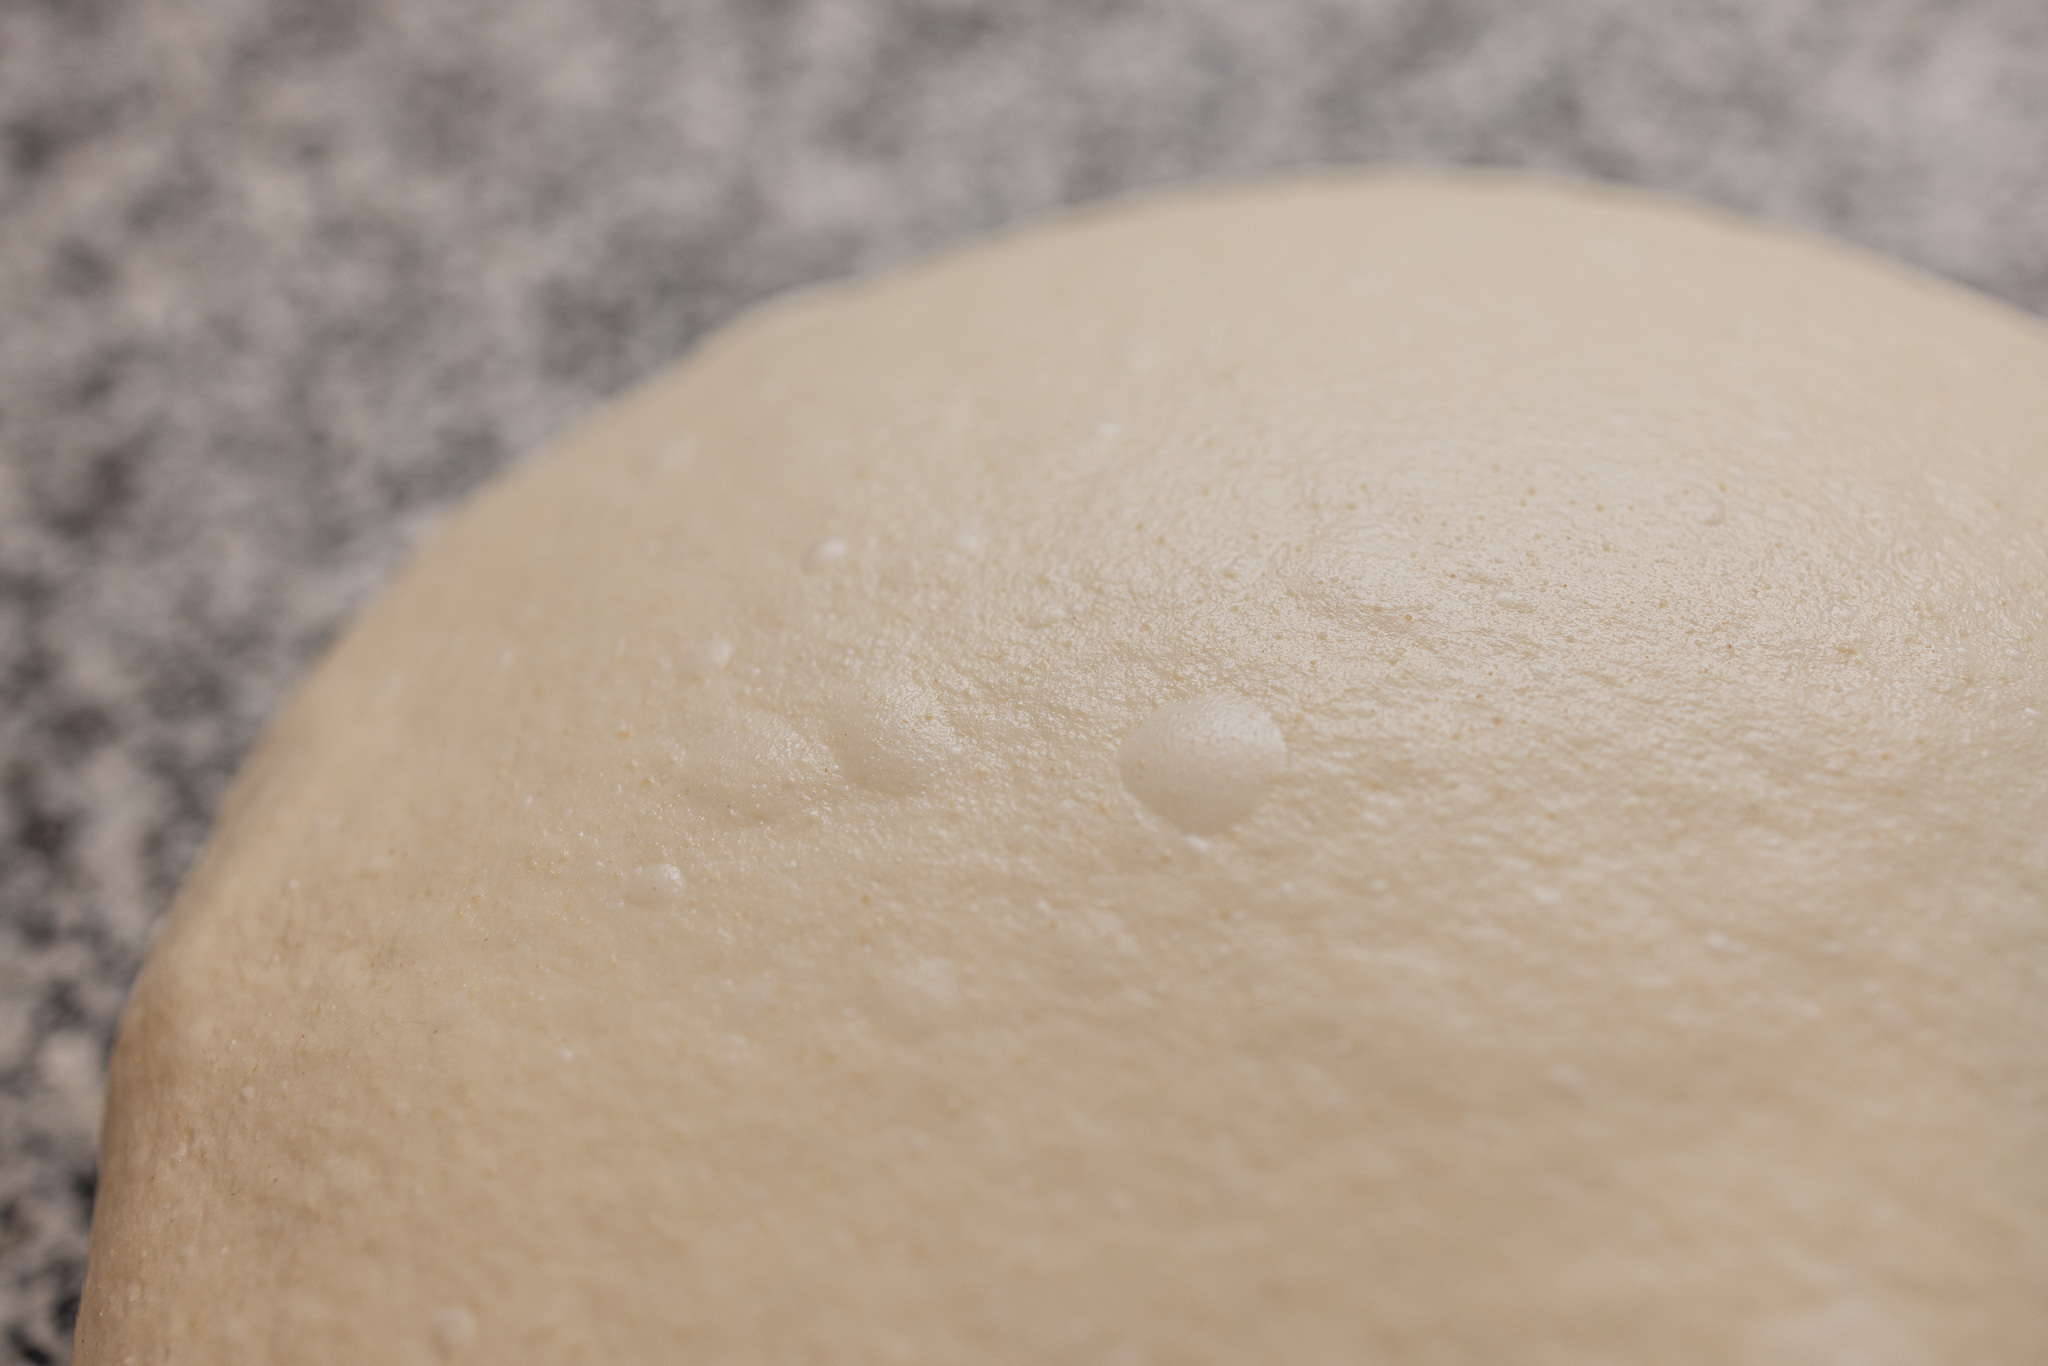
\includegraphics[width=\textwidth]{bulk-finished-dough}
  \caption[Dough at the end of bulk fermentation]{A dough in a good state to
      finish bulk fermentation. Notice the tiny bubbles on the dough's surface.
      They are a sign that the dough is inflated well enough.}
\end{figure}

Look out for bubbles on the surface of your dough. They
are a good sign that your dough is inflated with gas. The
further you push the bulk fermentation the more bubbles
will appear. If you overdo this stage, the dough becomes leaky, and
the bubbles will disappear again.

Take note of the dough's smell. It should match the same
smell of a ripe starter shortly before collapsing. As mentioned
before, your dough is nothing but a gigantic starter. You
can also proceed and taste your dough. It will taste like
pickled food. Depending on the acidity you can judge how
far the dough is in the fermentation process. The final bread
will taste less sour. That's because a lot of acidity evaporates
during baking\footnote{More on this topic later.
Just by baking longer and/or shorter, you can control
the tang of your final baked bread. The longer
you bake, the less sour the final loaf. The shorter,
the more acidity is still inside the bread. The resulting
loaf will be sourer.}.

When touching the dough, it should feel tacky
on your hands. The dough should also be less sticky
compared to earlier stages. If the dough is overly
sticky, you have pushed the fermentation too far.

If you pushed the bulk fermentation too far, you won't be able
to bake a freestanding loaf with the dough anymore. But don't
worry. You can move your dough into a loaf pan, or use parts
of the dough as the starter for your next dough. When using
a loaf pan, make sure it's properly greased. You might have
to use a spatula to transfer your dough. Allow the dough
to proof for at least 30~minutes in the loaf pan before
baking it. This makes sure that large cavities induced
by the transfer are evened out. You could push the proofing
stage to 24~hours or even 72~hours. The resulting
bread would feature an excellent, very tangy taste.


\section{Stretch and folds}

\begin{figure}[!htb]
  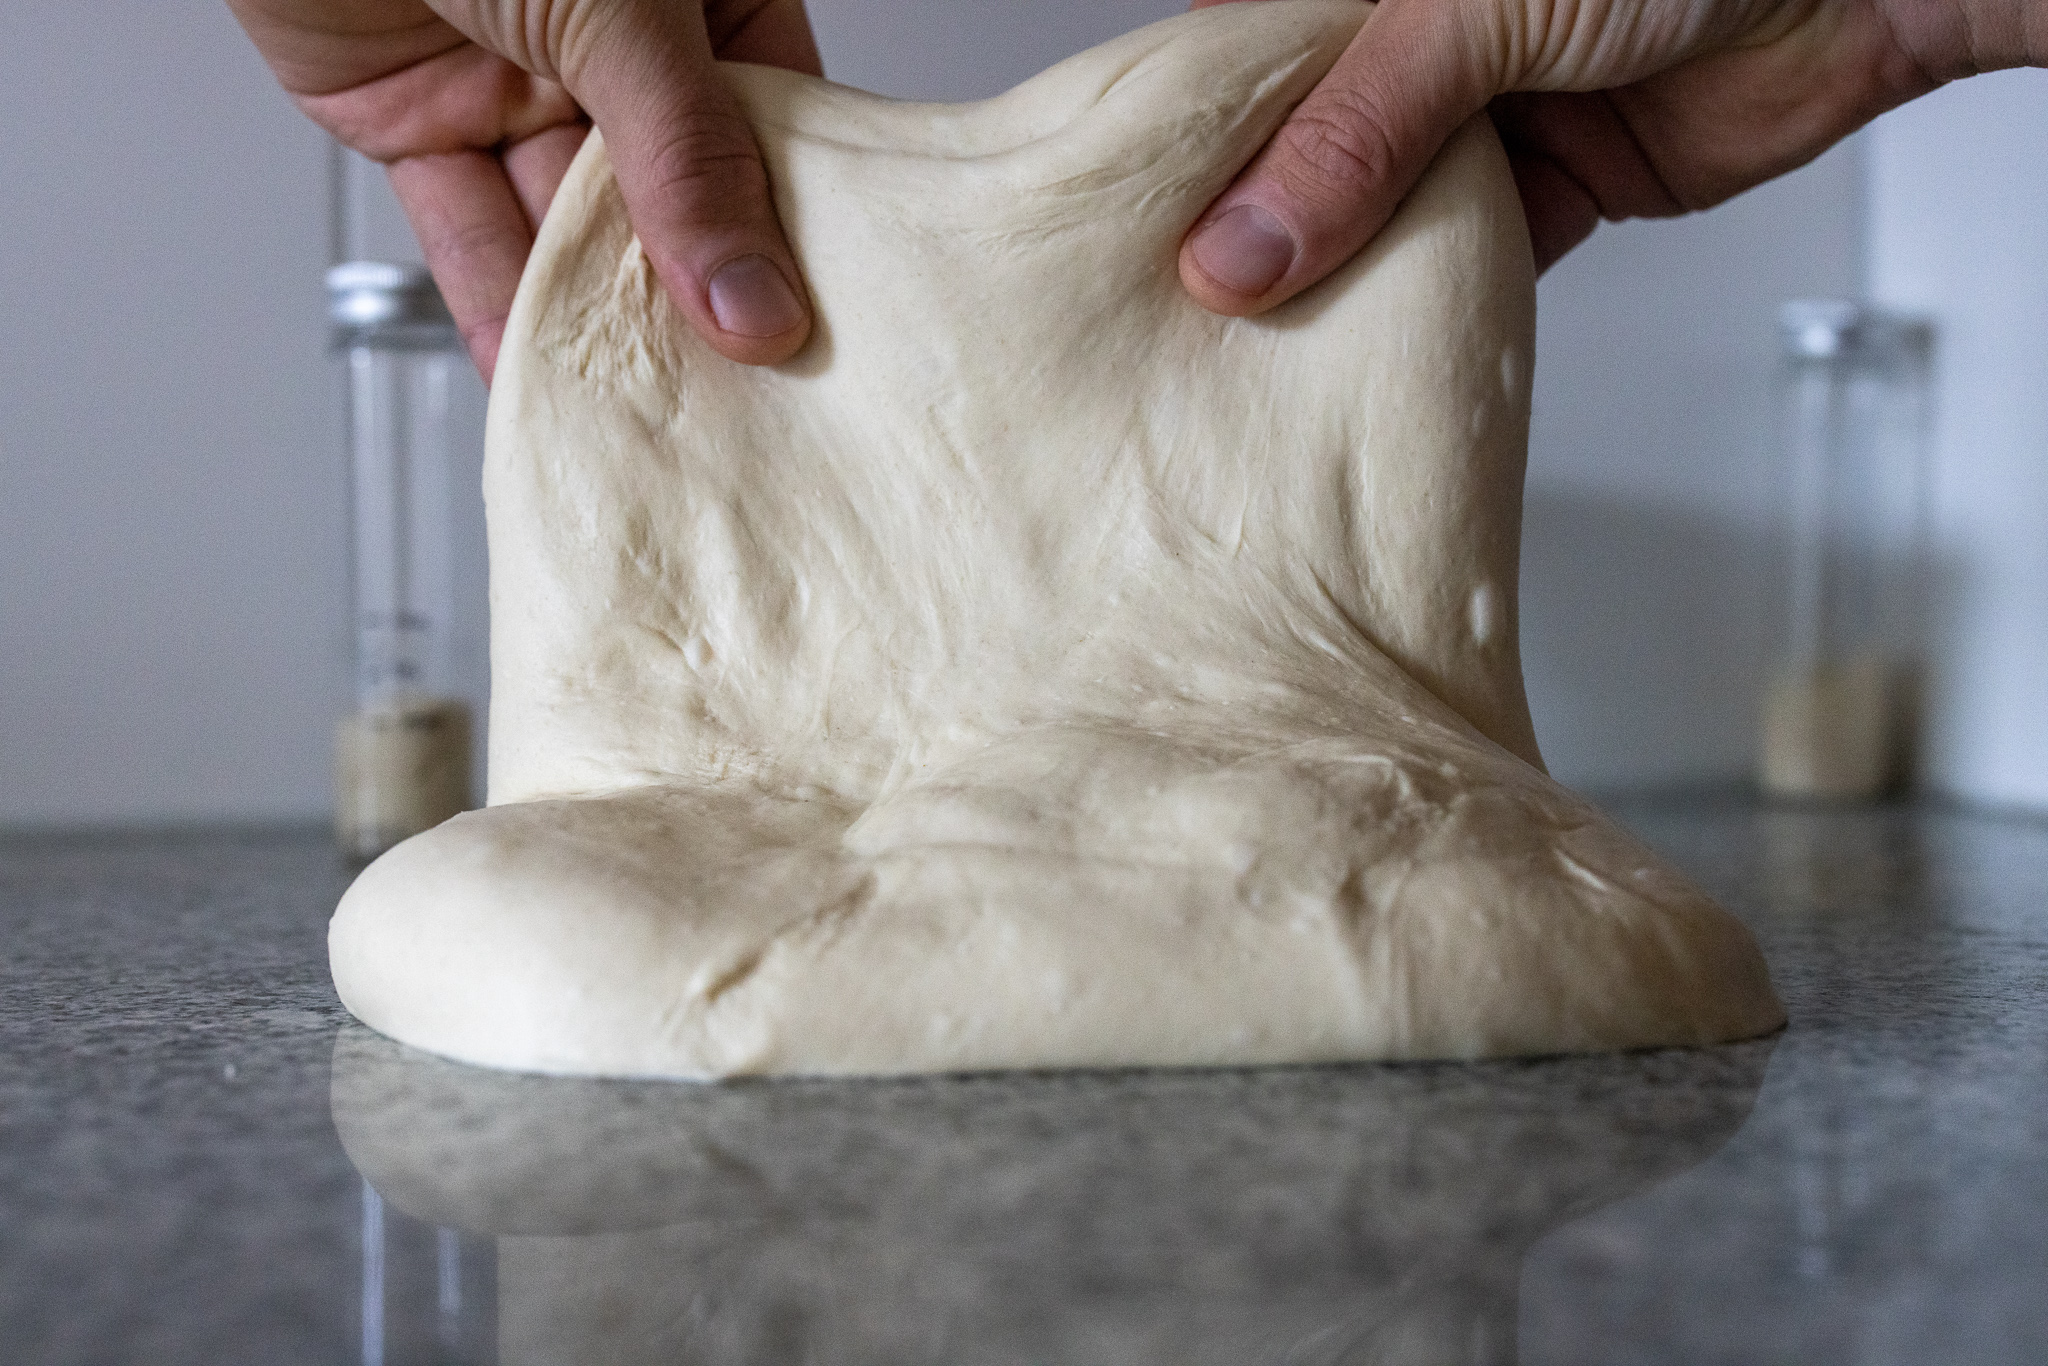
\includegraphics[width=\textwidth]{dough-being-glued}
  \caption[Gluing dough]{A dough where two sticky sides are being glued
      together using a stretch and fold. This process creates excellent dough
      strength.}
\end{figure}

In this section, you will learn all you need to know about stretching and
folding. You will learn when to stretch and fold and how to use this technique
to your advantage.

Stretching and folding is a set of techniques used by bakers during the bulk
fermentation stage. The process involves stretching the dough and then
folding the dough onto itself. Some recipes call for a single stretch
and fold, others for multiple.

The primary goal of this technique is to provide additional dough strength to
your dough. As shown in Figure~\ref{fig:dough-strength-sourdough} there are
multiple ways to create dough strength\footnote{In fact I~have seen many
    no-knead recipes calling for no initial kneading, but then applying
    stretch and folds during the bulk fermentation. The time required to do
    all the folds probably matches the initial kneading time required.}.
If you do not knead as much at the start, you can reach the same level of
dough strength by applying stretch and folds later. The more stretch and folds
you do, the more dough strength you add to your dough. The result will be a
more aesthetic loaf that has increased vertical oven spring.

Sometimes, if the dough is very extensible
and features very high hydration, stretching and folding is essential.
Without it, the dough itself would have too little dough strength and not
spring in the oven at all.

Another benefit of stretch and folds are their homogenization properties. By
folding the dough you are redistributing areas that are fermenting faster
than other areas. The heat in your dough is not the same in all areas.
The fermentation itself produces heat. For that reason, some of the areas in
your dough will ferment a little faster than others. This means that some
areas hold more gas and more acidity than others. Applying a stretch and fold
will redistribute heat, gas, and acidity. Some bakers also refer to this
process as crumb building. Careful folds ensure that your final dough's crumb
is not overly wild featuring large cavities. If you notice overly
large cavities in your final dough's crumb, then you might be able to fix that
by applying more stretch and folds\footnote{In many cases these cavities can
also happen when a dough does not ferment enough. The crumb is commonly called
Fool's Crumb. Refer to the later Debugging Crumb Structures chapter of this
book to learn more about it.}. Please refer to Section~\ref{section:debugging-crumb-structure}
``\nameref{section:debugging-crumb-structure}'' for more information on reading
your crumb.

\begin{figure}[!htb]
  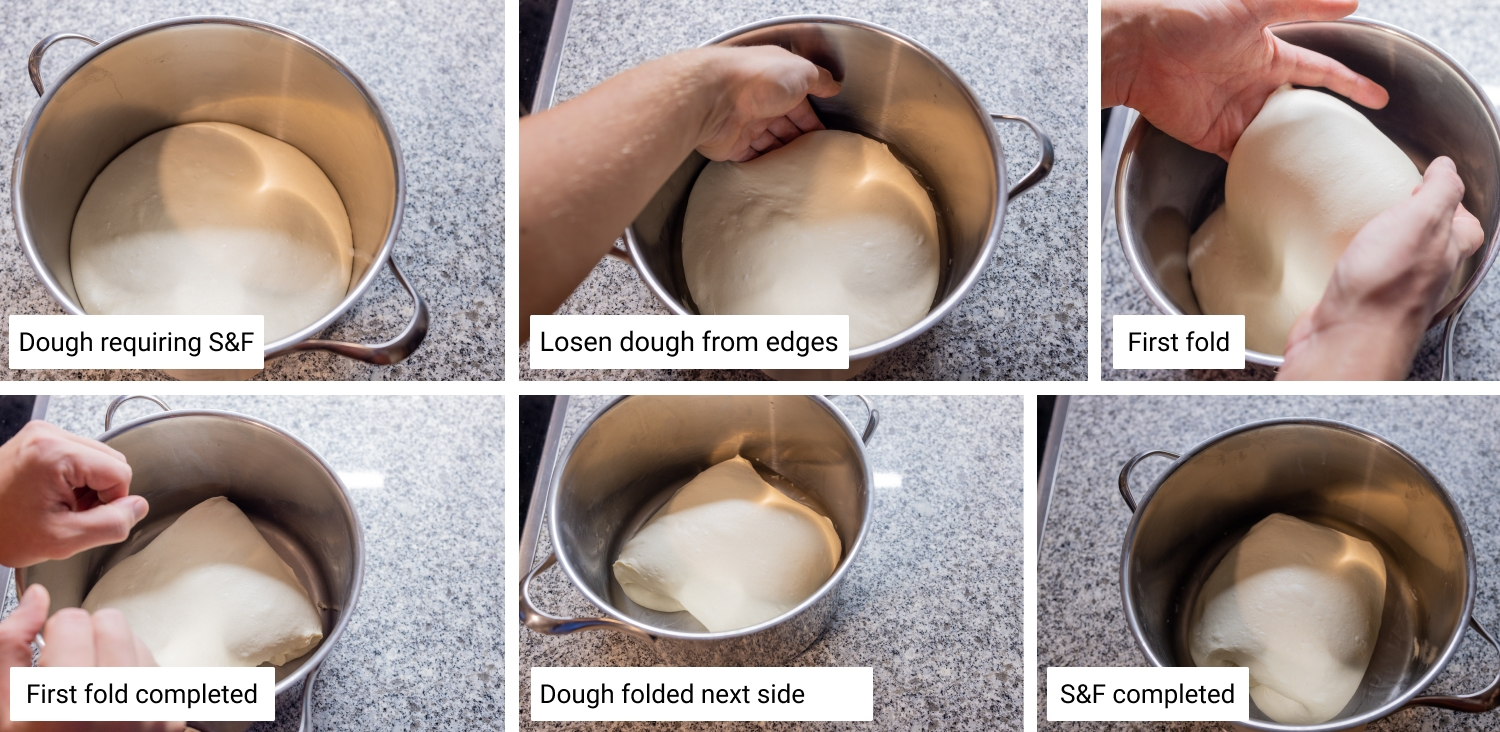
\includegraphics[width=\textwidth]{stretch-and-fold-steps}
  \caption[Stretch and fold steps]{An overview of the steps involved to perform
      stretch and folds for wheat-based doughs.}%
  \label{figure:stretch-and-fold-steps}
\end{figure}

The reason for the technique's popularity lies in its efficiency. By stretching
the dough outwards, you increase your dough's surface area. You then fold the
dough over, essentially gluing large areas of the dough together. Imagine a
piece of paper on which you place the glue. Then you fold the paper. Large areas
of the paper now stick together. Repeat the same process with more glue until
you have created multiple layers of paper and glue. This is the same thing that
happens to your dough. With only very few movements you have applied glue to your
dough.

To apply a stretch and fold first wet your hands with cold water. Watered hands
work wonders in reducing the dough's tendency to stick to your hands. Proceed and
carefully loosen the dough from the edges of your bulk container. Do this by
carefully placing your hand at the edge of the dough and pushing your hand
downwards on the container's walls. Once you have reached the bottom, drag the dough
a little bit inwards. The dough should stay in place and not move back to the
edge of your container. Try to be as swift as possible with this motion. The
slower you are, the more dough will stick to your hands. Repeat the same process
once all around your dough until the dough is free of your container's edges.
Wet your hands one more time and then carefully lift one side of the dough with
two hands placed in the center upwards. Make a fold in the center of the dough.
The upper smooth side needs to be placed on the bottom of the container. By doing
so, you will be gluing together the two sticky bottom sides. The top smooth side should
not be sticky in your hands, while the bottom rough surface should tend
to stick to your hands. Rotate the container
and repeat the same thing from the other side. Rotate the container 90°
and then repeat the process once again. Rotate the container another 180° in
the same direction
and repeat the fold one last time. By doing so you have applied 4 folds in total. Your
dough should now stay in place and resist flowing outwards\footnote{Please
also refer to~\cite{stretch+and+fold+technique} for a video showing you how to
best perform the technique.}.

In theory, there is no limit to how often you can stretch and fold. You could
apply one every 15~minutes. If your dough has enough dough strength already,
applying additional folds is just a waste of time\footnote{You could do it
just to better understand how the dough feels in your hands at different
fermentation stages.}. If you apply a large number of consecutive folds, the
outer layer of gluten
will tear. In that case, you just have to wait for at least 5--10~minutes until
the gluten bonds heal and you can try again. When the gluten does not heal
anymore, chances are you have pushed the fermentation for too long. Likely
most of the gluten has broken down and you are already
in the decay stage shown in Figure~\ref{fig:dough-strength-sourdough}.

\begin{figure}[!htb]
  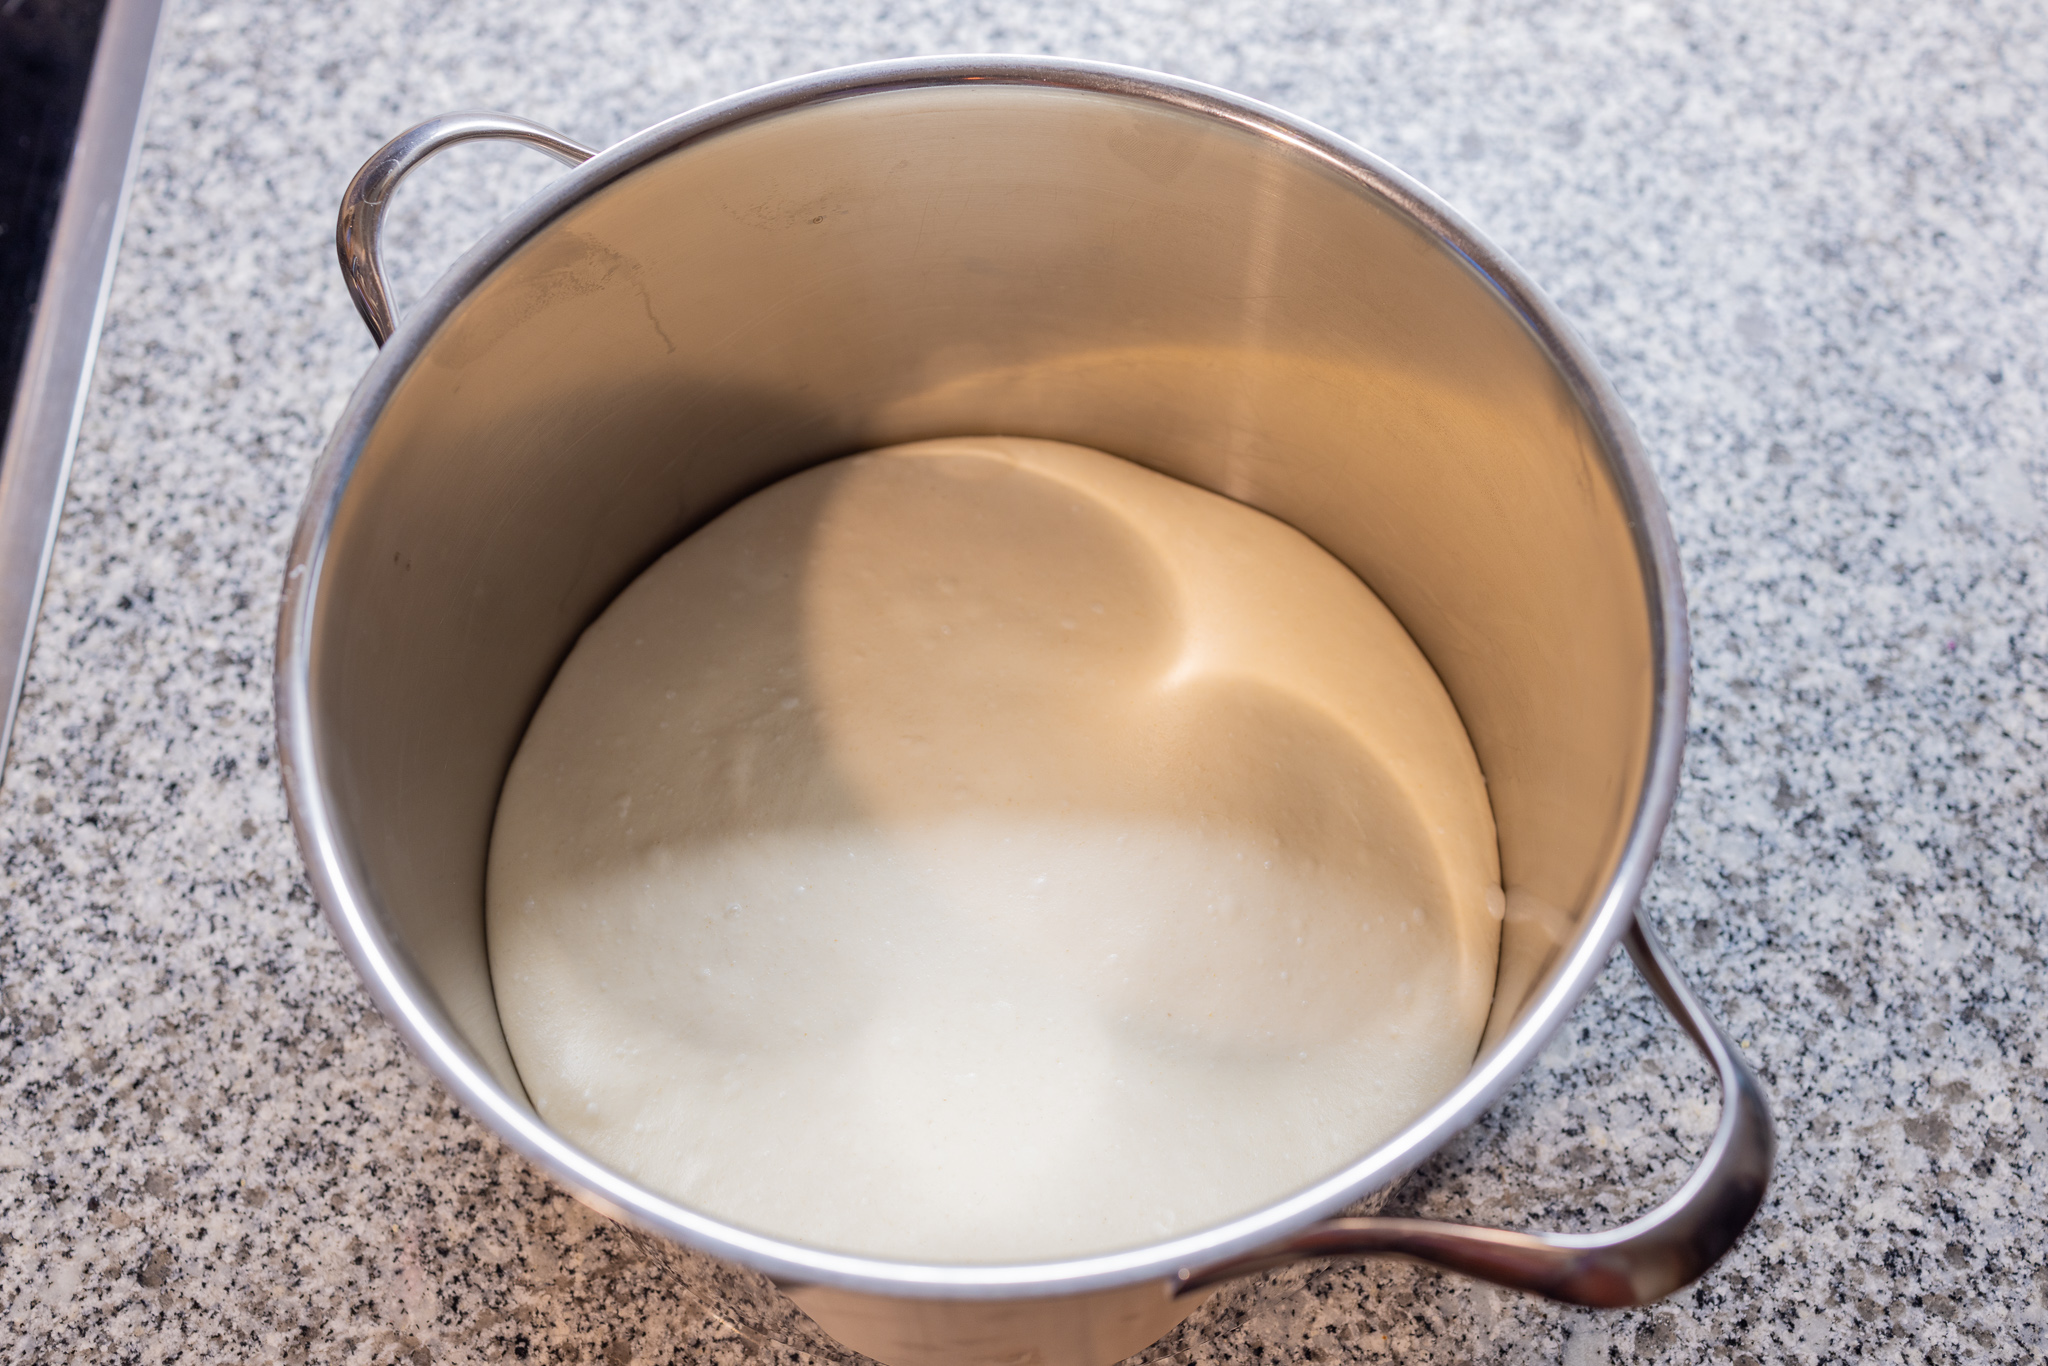
\includegraphics[width=\textwidth]{dough-requiring-stretch-and-fold}
  \caption[A flattened out dough]{A dough during bulk fermentation that has
      flattened out. To improve its dough strength, a stretch and fold should
      be applied.}
\end{figure}

Now, the reasonable amount of stretch and folds you should do greatly depends on how much you
kneaded initially and how extensible your dough is. A good recommendation is
to observe your dough in your bulk container. Once you see that the dough
flattens out quite a lot and spreads towards the edges of your bulk container,
you can proceed and apply a stretch and fold. For \qty{95}{\percent} of the doughs
that I~am making, this is hardly more than once. I~like to make overnight
doughs and in that case, I~typically apply one stretch and fold directly after
waking up. Then the bulk fermentation might take another 2~hours before I~proceed
with dividing and pre-shaping or directly shaping.

\section{Optional: Dividing and Preshaping}

Dividing and pre-shaping is an optional step that is done
once your sourdough finishes with the bulk fermentation stage.
The step is required if you are making multiple loaves in one
batch. It is optional if you are making a single loaf.

\begin{flowchart}[!htb]
\centering
  \begin{tikzpicture}[node distance = 3cm, auto]
  \node [start] (init) {\footnotesize Dividing required?};
  \node [decision, right of=init, node distance=5cm] (more_than_one_loaf) {\footnotesize More than 1 loaf?};
  \node [success, right of=more_than_one_loaf, node distance=5cm] (yes) {\footnotesize Yes};
  \node [success, below of=yes, node distance=3cm] (no) {\footnotesize No};
  \path [line] (init) -- (more_than_one_loaf);
  \path [line] (more_than_one_loaf) -- (yes);
  \path [line] (more_than_one_loaf) -- (no);
\end{tikzpicture}

  \caption[Is dividing your dough required check]{Dividing is only required when you are
      making multiple loaves in a single dough batch.}%
  \label{fig:dividing-decision-tree}
\end{flowchart}

The goal of dividing your dough into smaller pieces is to portion
your dough accordingly. This way you'll have multiple pieces of bread
which all weigh the same. For this reason, a scale is commonly
used to weigh the pieces of dough. If one piece of dough weighs
too little you can simply cut a bit more from your dough blob
to increase its weight.

When cutting the dough, try to be as concise as possible with your
movements. You don't want to unnecessarily damage your dough too much.
Quick movements with a knife or dough scraper help to prevent the
dough from sticking too much to your tools.

\begin{figure}[!htb]
  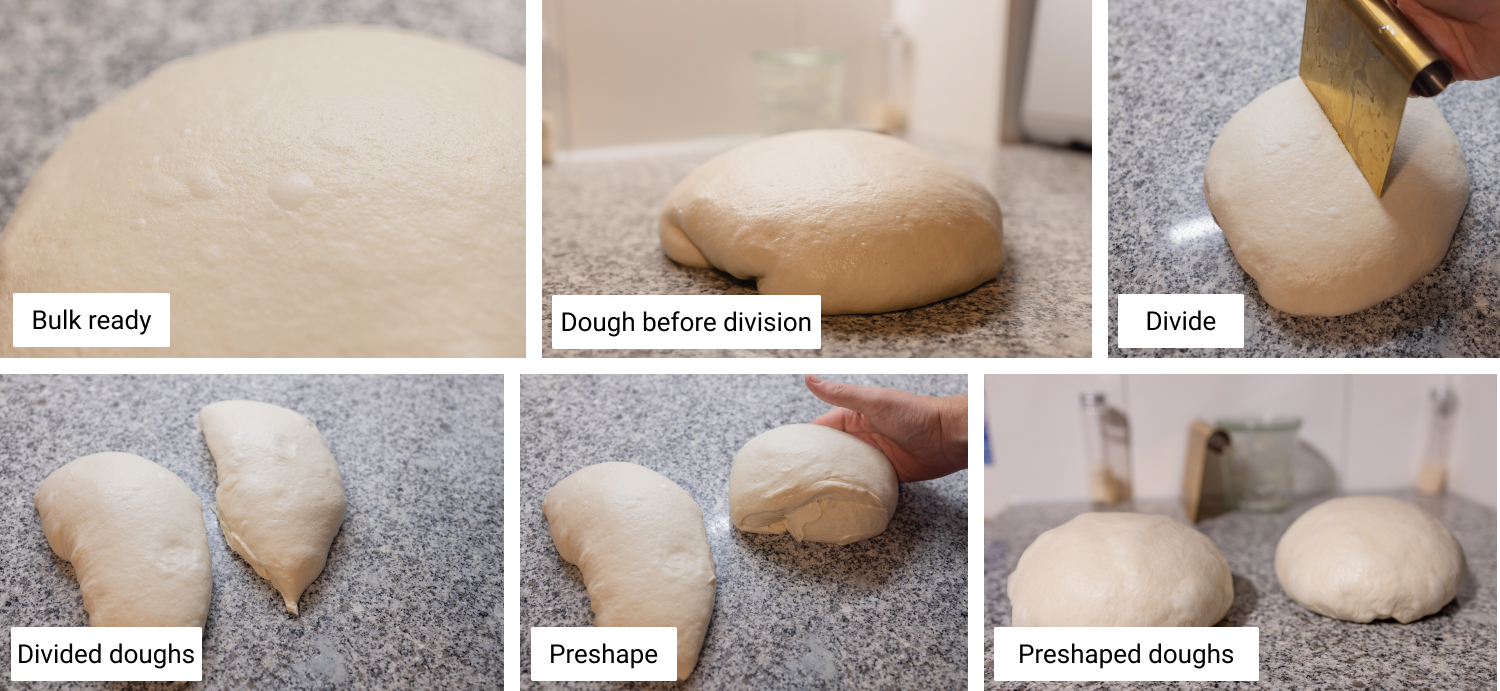
\includegraphics[width=\textwidth]{divide-preshape}
  \caption{The steps of dividing and preshaping your dough.}
\end{figure}

I~sometimes like to draw small lines with the dough scraper's edge
on the large dough mass before cutting it into smaller pieces.
This helps me to better plan where I~want to do my incisions. When
I~plan to make 8 loaves I~try to use the lines to divide the dough
into 8 equally sized portions before cutting. If this is not precise enough,
you can use the aforementioned scale.

Now that you have cut your dough, the resulting chunks are not in an equal shape.
This is problematic for the next stage when you are shaping your dough.
The resulting loaves wouldn't look nice and even. You would probably
end up with areas that tear the moment you are shaping your dough.
You wouldn't start the whole proofing process on a good foundation. For that
reason, you need to pre-shape your dough.

Pre-shaping is done for several reasons:
\begin{itemize}
  \item You divided your dough and require pre-shaping
  \item Your dough lacks dough strength. Pre-shaping will add more strength
  \item You want to even out the final loaf's crumb structure. By pre-shaping,
  the resulting crumb will look more even.
\end{itemize}

If you are making a single loaf from one dough batch the step is not required.
In that case, you can directly proceed with shaping, skipping this step.

The pre-shaping technique is the same as the process
Figure~\ref{fig:dough-ball-steps}.  Whereas earlier you could tear the dough's
surface this could now result in a catastrophe.  For this reason, I~recommend
practicing this step for as long as you need after kneading.  The gluten
network might be so extensible and degraded at this point that there is hardly
any room for error. The dough wouldn't come together again. The only way to
save such dough is to use a loaf pan.

\begin{figure}[!htb]
  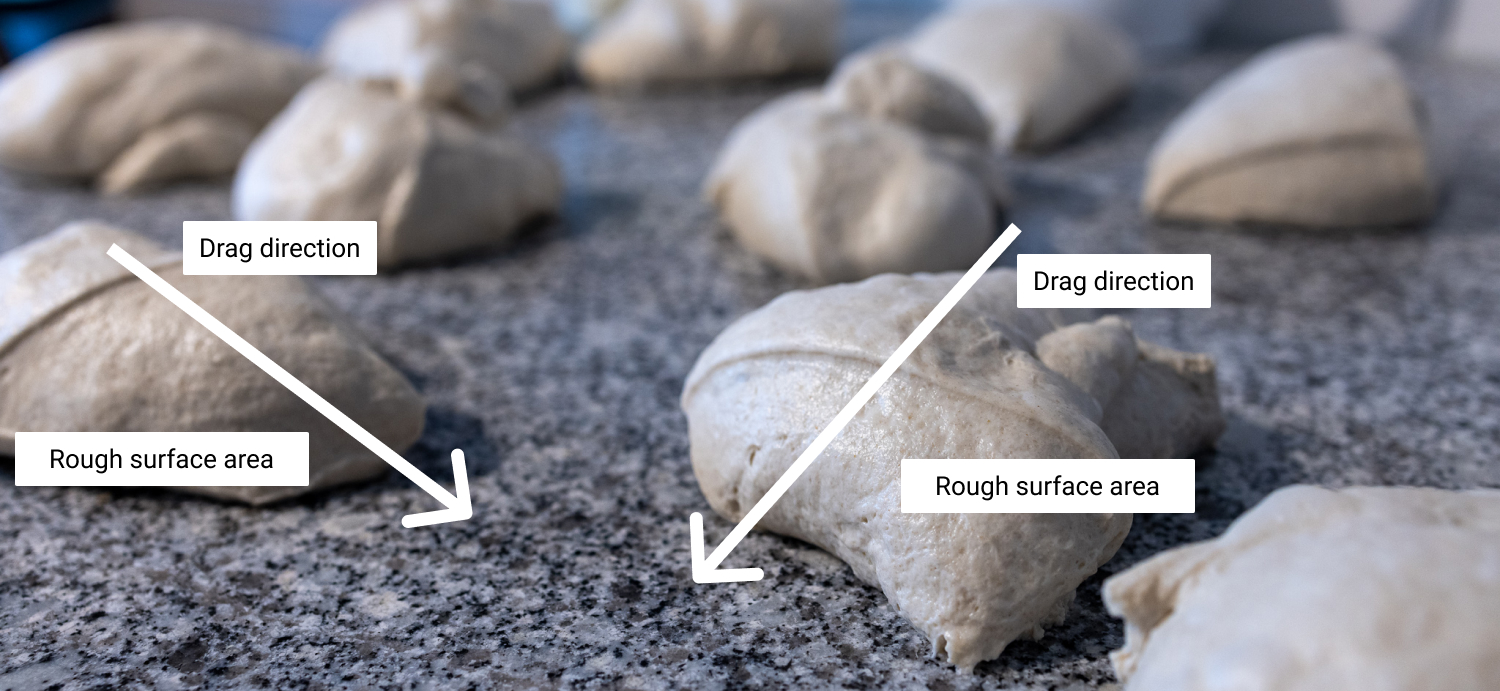
\includegraphics[width=\textwidth]{preshape-direction}
  \caption[Dragging direction]{Drag the dough in the direction of the rough
      surface area. This way you minimize the movements required to complete
      the step.}%
  \label{fig:preshape-direction}
\end{figure}

Pre-shape the dough as much as is needed to round up the top surface area. Try
to touch the dough as little as possible to reduce its ability to stick to
your hands. Drag the dough in the direction where you see a rough surface
area. In case you have too little space to drag the dough because it might
fall from the edge of your counter, simply lift it with a swift movement and
place it in a better position for pre-shaping. Please refer to
Figure~\ref{fig:preshape-direction} for a visualization showing the
pre-shaping direction.

Try to set yourself a limit of movements to finish pre-shaping
a dough. Then you will be more conscious about each movement
you are performing. At the start you can try 5 movements,
iteratively reducing this to 3. The only reason for exceeding these
numbers could be if you on purpose want to even out the crumb
structure of your final loaves further.

\begin{figure}[!htb]
  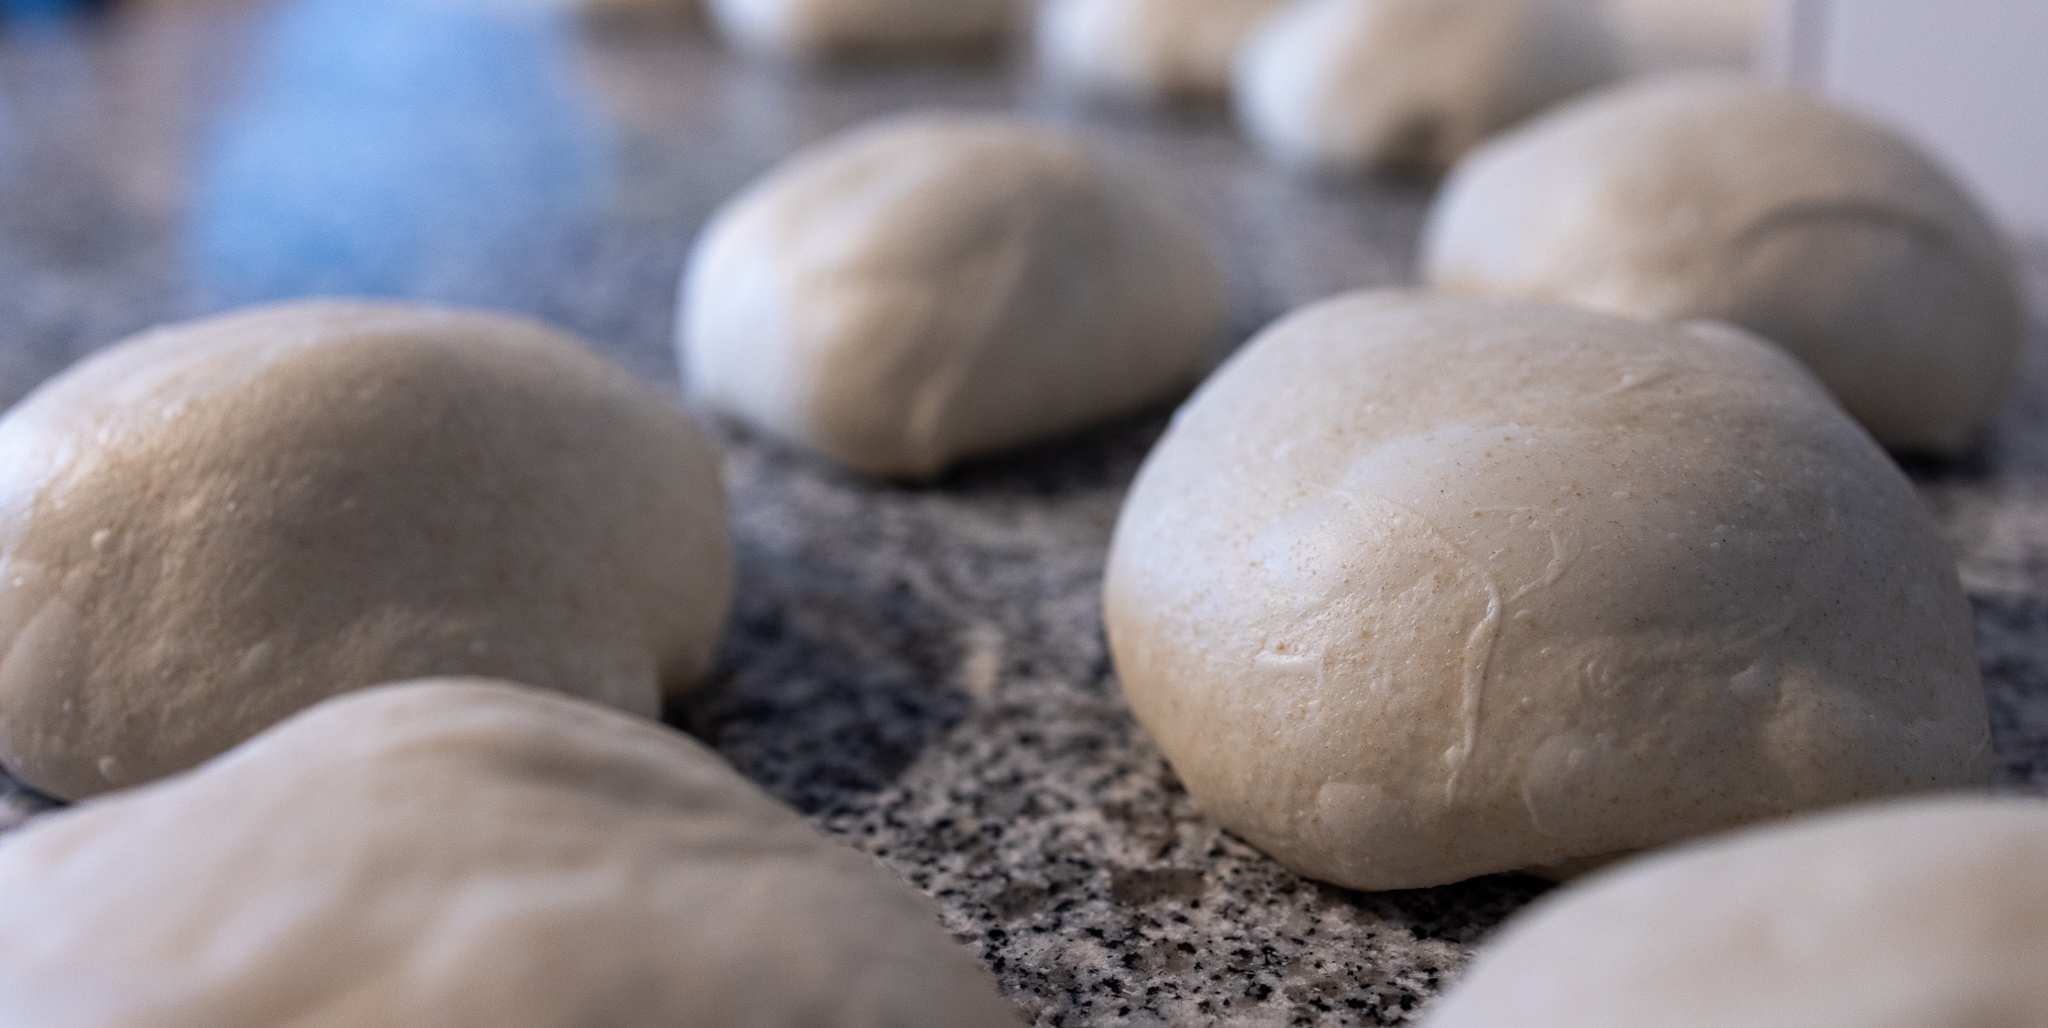
\includegraphics[width=\textwidth]{preshaped-dough}
  \caption{Baguette doughs resting after preshaping.}%
  \label{fig:dough-after-preshaping}
\end{figure}

Once you finished pre-shaping allow the dough balls to rest
on your counter for at least 10--15~minutes. Do not
cover the pre-shaped balls. By drying out the surface,
the following shaping step will be easier. The dried-out surface
will not stick to your hands as much. As
you tightened the dough's gluten you will need to
allow it to relax. Without a resting period, you wouldn't
be able to shape your dough into, for instance, a baguette-like structure.
The dough would resist each movement
always springing back into the previous shape. You
might have noticed this before, when making pizza dough. If you
don't wait long enough after balling the pizzas, it's impossible
to stretch the pizza. By waiting a few more minutes,
stretching becomes a lot easier. The dough will not resist
being transformed into the final shape that you like.

The aforementioned 10--15~minutes bench rest time depends
on how strongly you pre-shaped your dough. The more
you pre-shape the longer you need to wait. If your dough
resists a lot during shaping, extend this period up to 30~minutes.
If you wait too long, your dough's surface area can become too dry,
resulting in the dough tearing during shaping. As always, please
take these timings with a grain of salt and experiment in
your environment.

\section{Shaping}

\begin{flowchart}[!htb]
\centering
  \begin{tikzpicture}[node distance = 3cm, auto]
  \node [block] (init) {\footnotesize Begin shaping};
  \node [decision, right of=init, node distance=5cm] (overfermented_decision) {\footnotesize Dough overly sticky or dough tears?};
  \node [block, right of=overfermented_decision, node distance=4cm] (overfermented) {\footnotesize Your dough is likely overfermented};
  \node [block, right of=overfermented, node distance=3cm] (loafpan) {\footnotesize Move to loaf pan, short proof, then bake directly};
  \node [block, below of=init, node distance=4cm] (shaping_technique) {\footnotesize Proceed with shaping technique};
  \node [block, right of=shaping_technique, node distance=3cm] (flour) {\footnotesize Flour shaped dough};
  \node [block, right of=flour, node distance=3cm] (banneton) {\footnotesize Place upside down in banneton};
  \node [block, right of=banneton, node distance=3cm] (proof) {\footnotesize Begin proofing};
  \path [line] (init) -- (overfermented_decision);
  \path [line] (overfermented_decision) -- node{yes} (overfermented);
  \path [line] (overfermented_decision) -- node{no} (shaping_technique);
  \path [line] (shaping_technique) -- (flour);
  \path [line] (flour) -- (banneton);
  \path [line] (banneton) -- (proof);
  \path [line] (overfermented) -- (loafpan);
\end{tikzpicture}

  \caption[Sourdough shaping process]{A schematic visualization of the shaping process
      including checks for an overfermented dough.}%
  \label{fig:shaping-decision-tree}
\end{flowchart}

Shaping will give your dough the final shape before baking. After
completing shaping, your dough proceeds to the proofing stage and
will then be scored and ultimately baked.

There are countless shaping techniques. The technique to choose
depends on the type of bread you want to make. Some techniques
are gentler on the dough, making sure that the dough does not
degas. Other techniques are faster but degas the dough a little
more. The tighter you shape, the more evened out your final dough's
crumb structure will look. At the same time, a tighter shaping-technique
will improve your dough's strength. More strength will ultimately result
in more vertical oven spring.

The following instructions assume that you want to make a batard-style
bread featuring an oblong shape. Learning this technique
will provide you with a solid knowledge foundation that
can easily be extended to make bread rolls or baguettes.

Mastering the challenging shaping technique will likely take you
multiple attempts. You only have a single attempt per dough, though. If you
make a mistake, the final bread is likely not going to turn out as good
as it could. If this technique causes you a headache, I~recommend making
a larger batch of dough and dividing and preshaping it into
smaller portions. Instead of making a large batard, practice making miniature
batard bread rolls.

\subsection[Flouring the surface]{Apply flour to the dough's surface.}

\begin{figure}[!htb]
  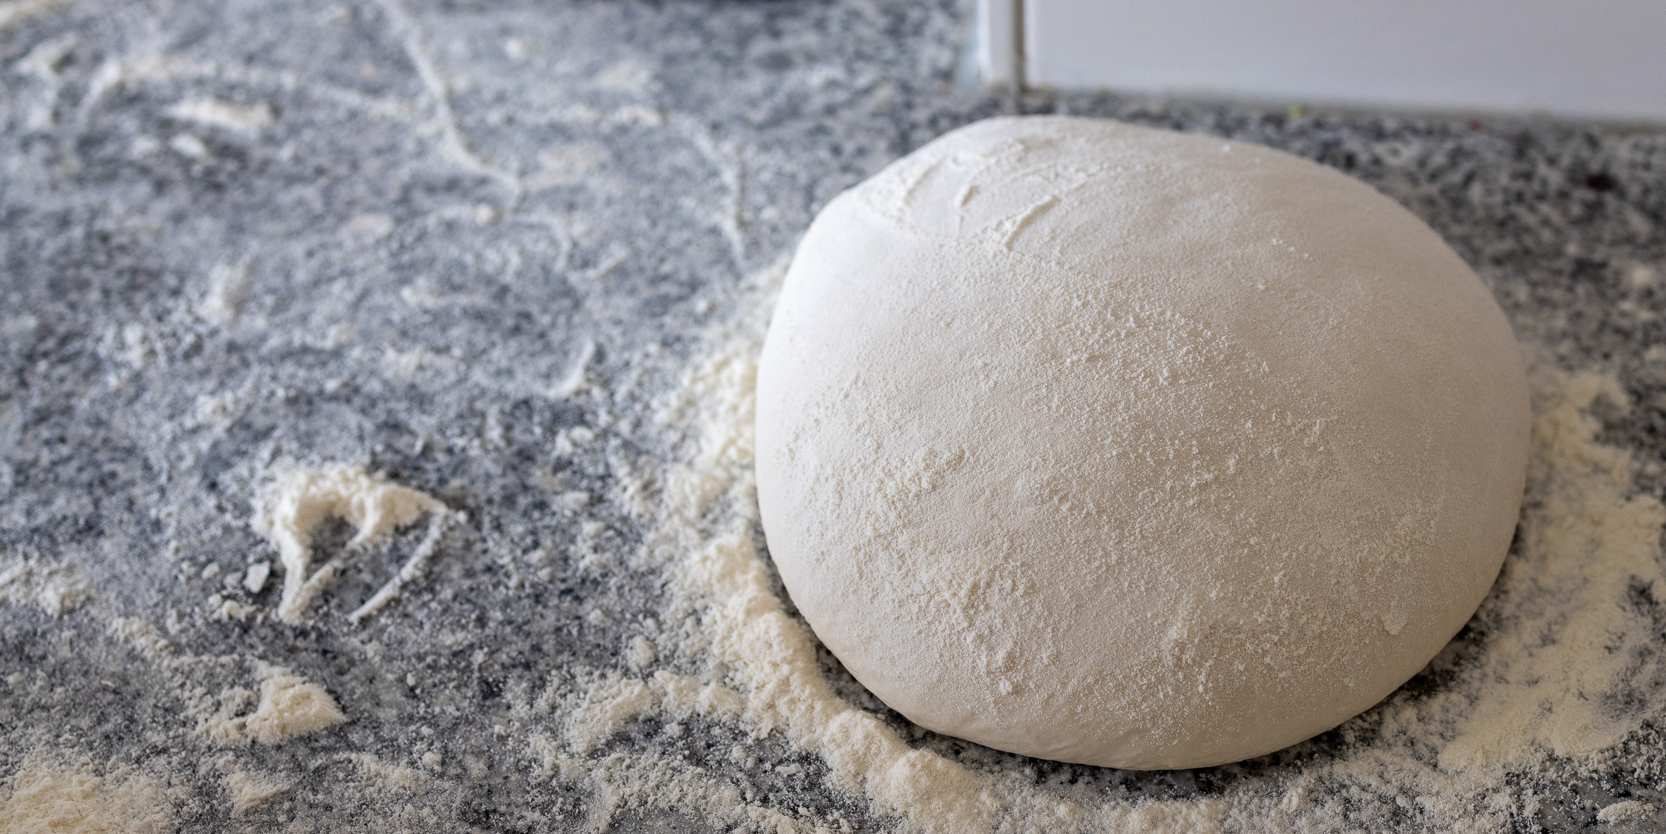
\includegraphics[width=\textwidth]{step-1-flour-applied}
  \caption[Step 1 of shaping process]{A dough that has flour applied to its
      surface. This is the first step of the shaping process.}%
  \label{fig:shaping-flour-surface}
\end{figure}

If you are only making 1 loaf out of your dough, apply flour
generously to the top layer of your dough. Rub the flour onto your
dough with your hands. Flip over your container. Wait a little bit
to allow the dough to release itself from the container. Proceed
with step 3.

If you divided and pre-shaped, apply flour generously to the dough's
top layer as well. With gentle hands spread the flour evenly across
the dough's surface. See Figure~\ref{fig:shaping-flour-surface} for a
visual representation of how your dough should look after coating
the surface.

\subsection[Flipping the dough]{Flip the dough over}

\begin{figure}[!htb]
  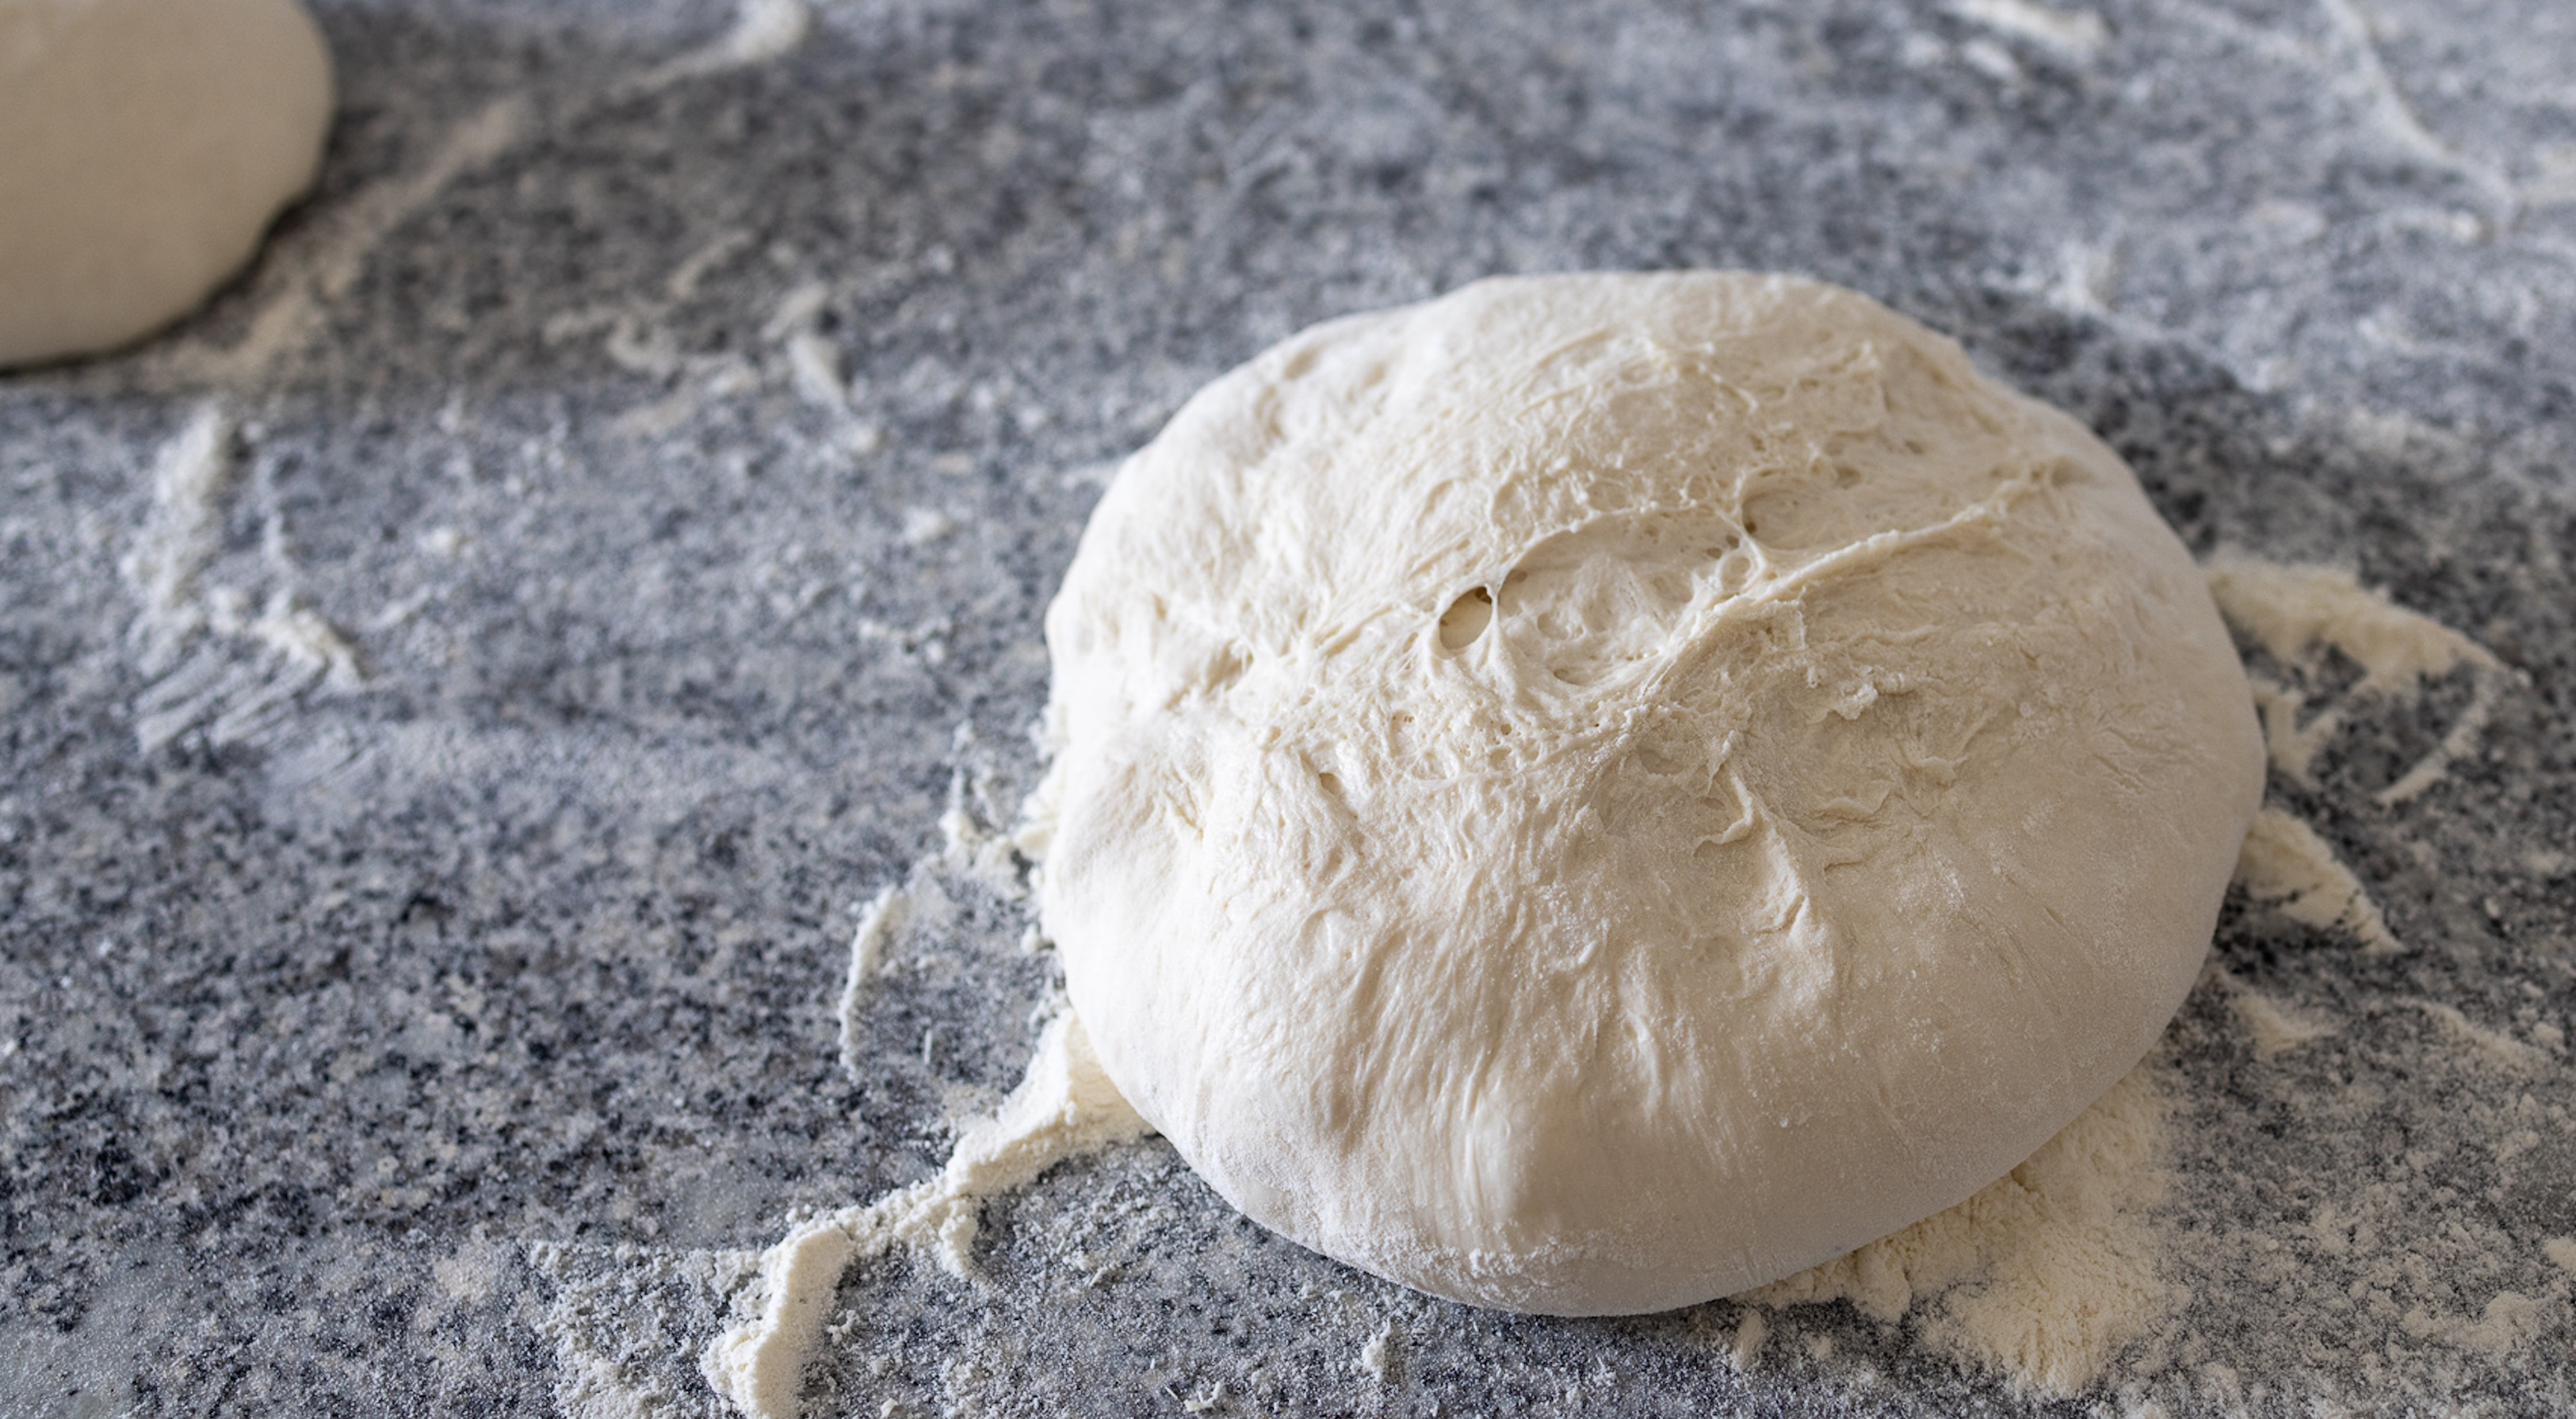
\includegraphics[width=\textwidth]{step-2-flipped-over}
  \caption[Step 2 of shaping process]{A flipped-over dough. Note how the
      sticky side is facing you while the floured side is facing the
      countertop.  The sticky side is used as glue to hold the dough together.}
\end{figure}

With gentle hands, carefully remove the dough from the surface. If
you possess a dough scraper, carefully tuck it under the dough with
rapid movements. Flip the dough over, making sure that the floured
areas are in contact with your hands. The non-floured bottom area that was
stuck to the counter is a no-touch zone. Try to avoid touching it
as it is rough and thus will stick to your hands.

Gently proceed and place the dough with the previously top-facing side
on your counter. The floured area is now on the surface, whereas the
sticky side is facing you.

\subsection[Create rectangular shape]{Make the dough rectangular}

\begin{figure}[htb!]
  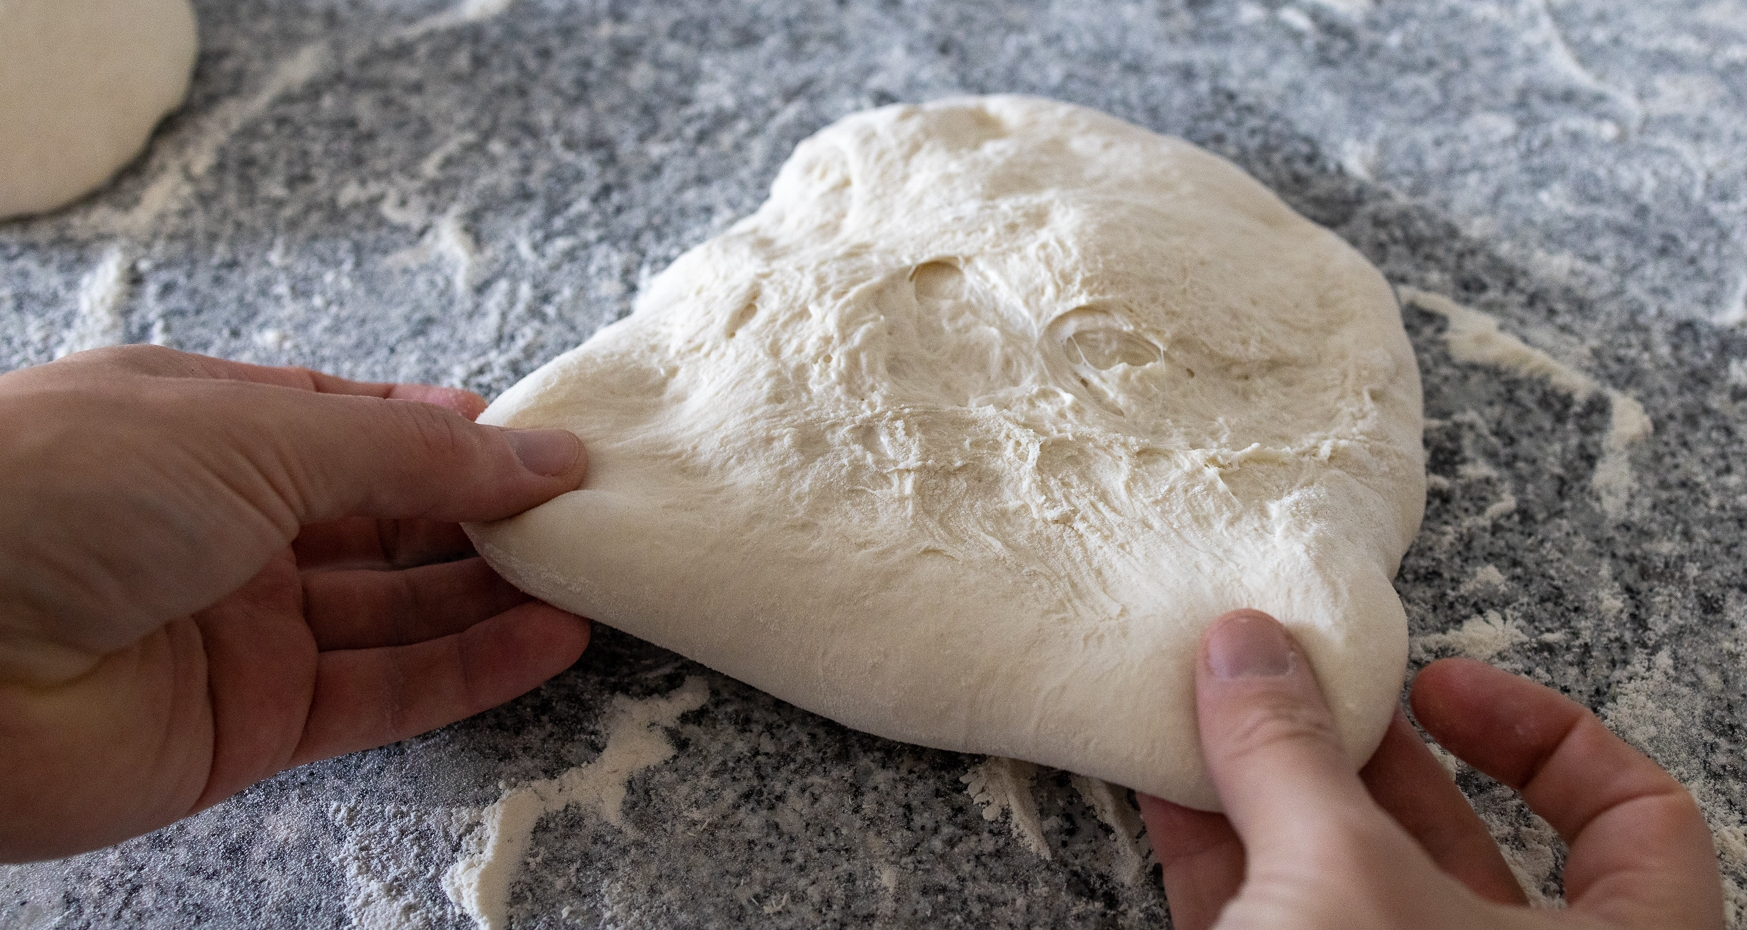
\includegraphics[width=\textwidth]{step-3-rectangular}
  \caption[Step 3 of shaping process]{A flipped-over dough. Note how the
      sticky side is facing you while the floured side is facing the
      countertop.}%
  \label{fig:shaping-rectangular-dough}
\end{figure}

You should be facing the sticky side of your dough now. Note how
the dough is currently round and not rectangular. The circular
shape will not be ideal when shaping the oblong batard.

For this reason, proceed and stretch the dough a little bit until
it has a more rectangular shape. While stretching, make sure to touch
the sticky side as little as possible. Place your hands on the bottom
floured side and the edge of the sticky side. With gentle hands,
stretch the dough until the shape in front of you looks rectangular.
Refer to Figure~\ref{fig:shaping-rectangular-dough} and compare
your dough with the shown dough.

\subsection[Folding]{Fold the dough together}

\begin{figure}[htb!]
  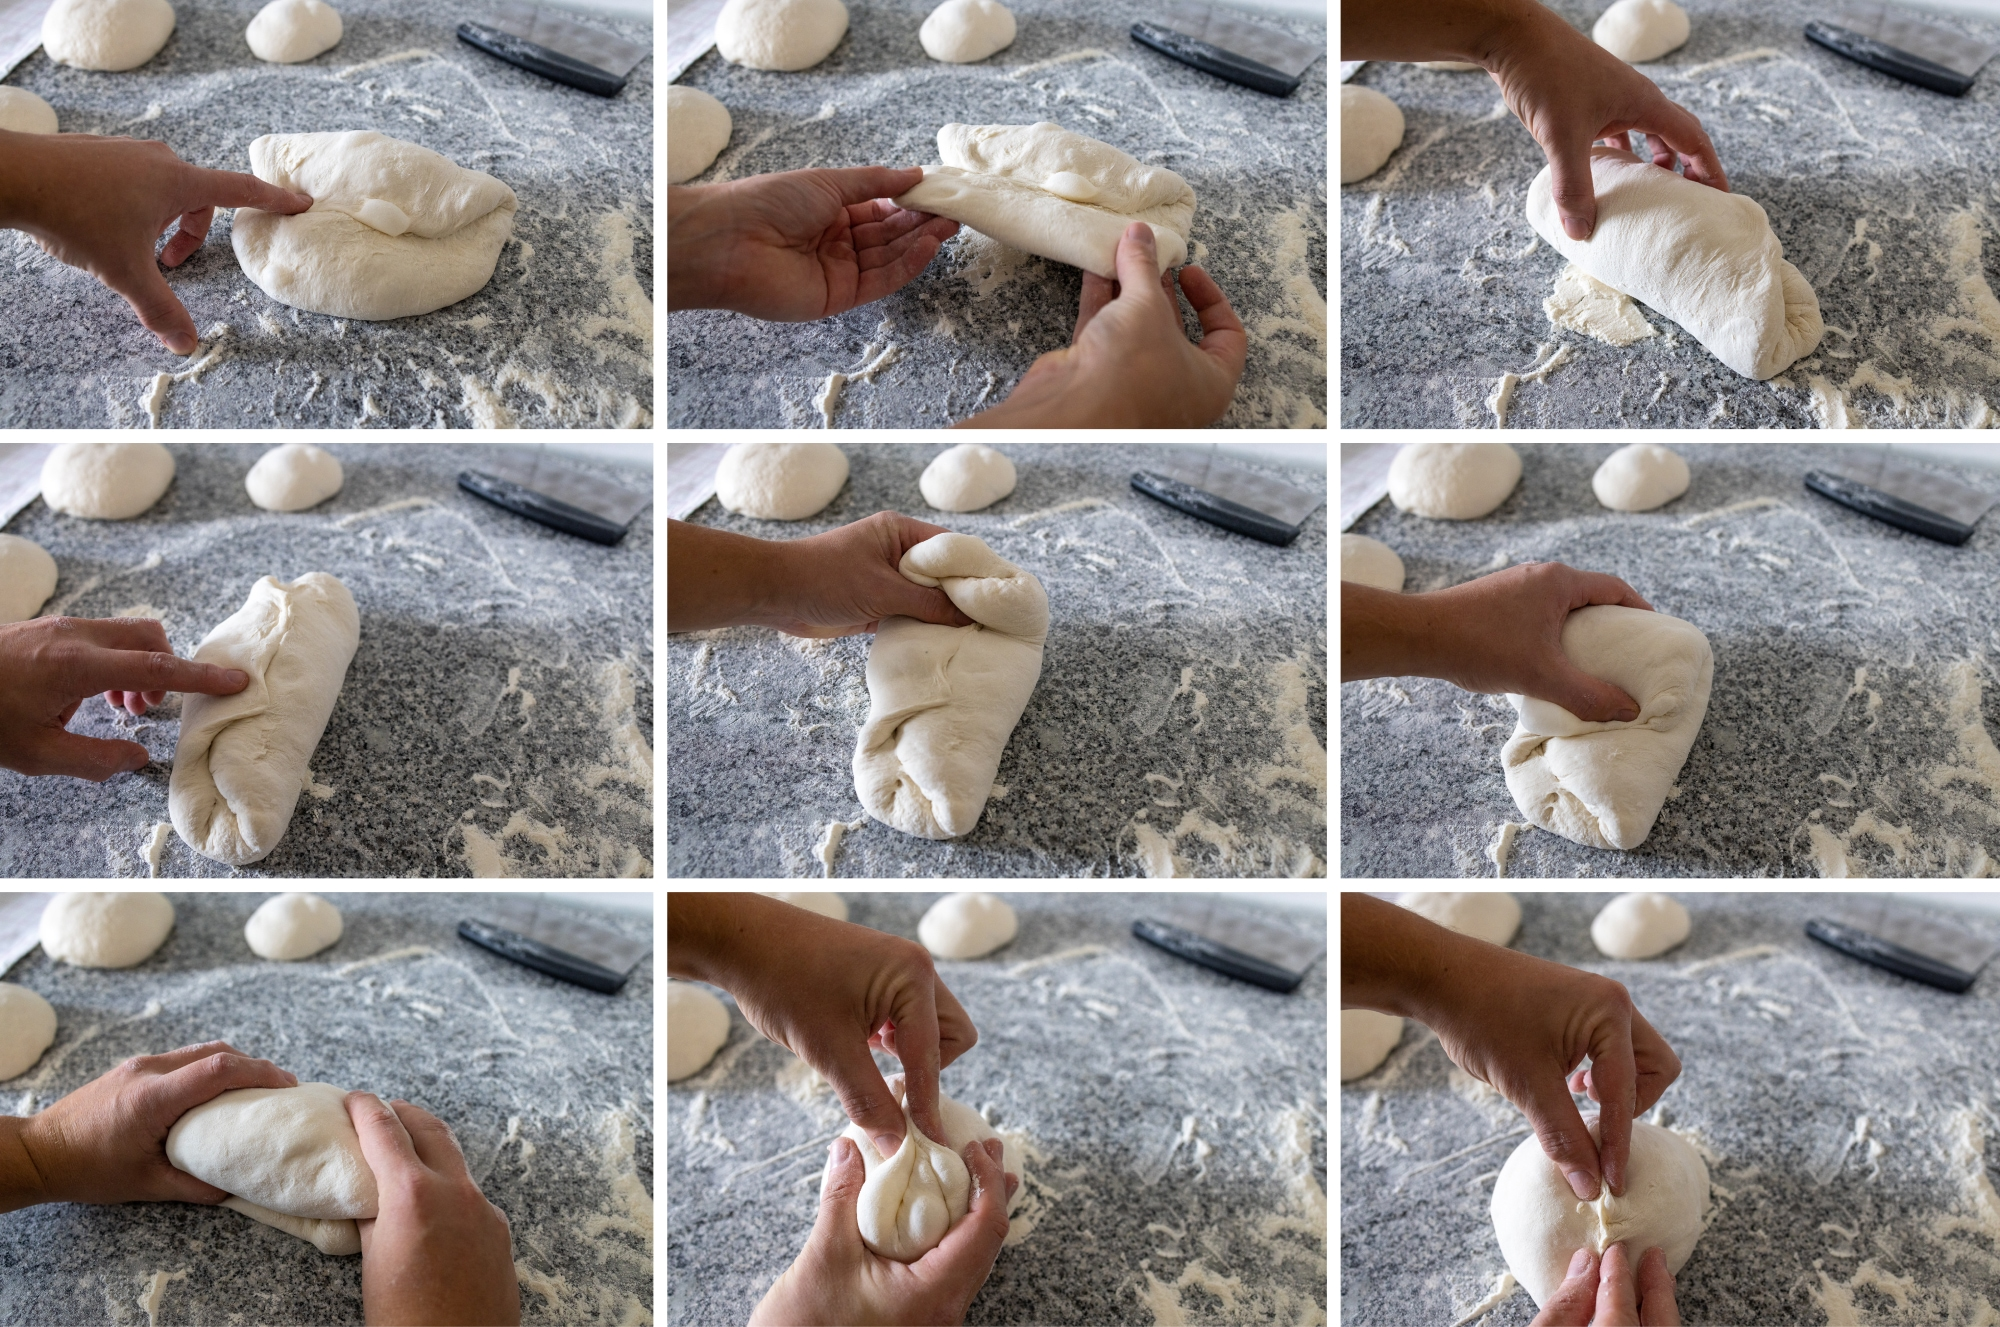
\includegraphics[width=\textwidth]{step-4-folding}
  \caption[Step 4 of shaping process]{The process of folding a batard. Note
      how the rectangle is first glued together and then rolled inwards to
      create a dough roll. Ultimately the edges are sealed to create a more
      uniform dough.}%
  \label{fig:shaping-folding}
\end{figure}

Now that you have created the rectangular shape, your dough
is ready to be folded together. This only works because the side
facing you is sticky. Because of the dough's stickiness,
we can effectively glue it together, creating a very
strong bond.

You can practice this step with a piece of rectangular paper.
Once you mastered folding on paper you can easily apply
this to your real-life dough.

Make sure the batard is placed in front of you. Take the side
that faces you and fold it into the middle of the dough. Carefully
tuck it down so that it glues together with the sticky side.

Take the other side and fold it over the side you just folded.
Stretch the dough as much as possible towards you. Tuck it down
on the edge, creating your first glue layer.

Rotate the dough so that it is aligned lengthwise in front of you.
Rotate the dough inwards so that the seam side
now faces you.

Start to roll the dough inwards beginning at the top of the dough.
Keep rolling the dough inwards until you have created a dough roll.

Refer to Figure~\ref{fig:shaping-folding} for a full visual
representation of the process.

If your dough does not hold its shape, chances are you have pushed
the fermentation too far. Most of the gluten has been degraded
and the dough won't be able to hold its shape. In this case,
the best option is to use a loaf pan to bake your bread. The
final bread will taste amazing but not offer the same texture
a freestanding bread would offer. Please refer to
Section~\ref{section:debugging-crumb-structure} for more
details on how to properly read your dough's crumb structure.

\subsection[Sealing]{Sealing the edges}

Your dough has finished shaping now. Sealing the edges
is an optional step. I~like to do it because, in my opinion,
the final baked bread will look a little bit nicer without
any rough edges.

Gently pull together the swirl-like-looking edges of your dough
with two fingers. Rotate the dough and then repeat the same process
from the other side as well.

\subsection[Proofing preparation]{Prepare for proofing}

\begin{figure}[htb!]
  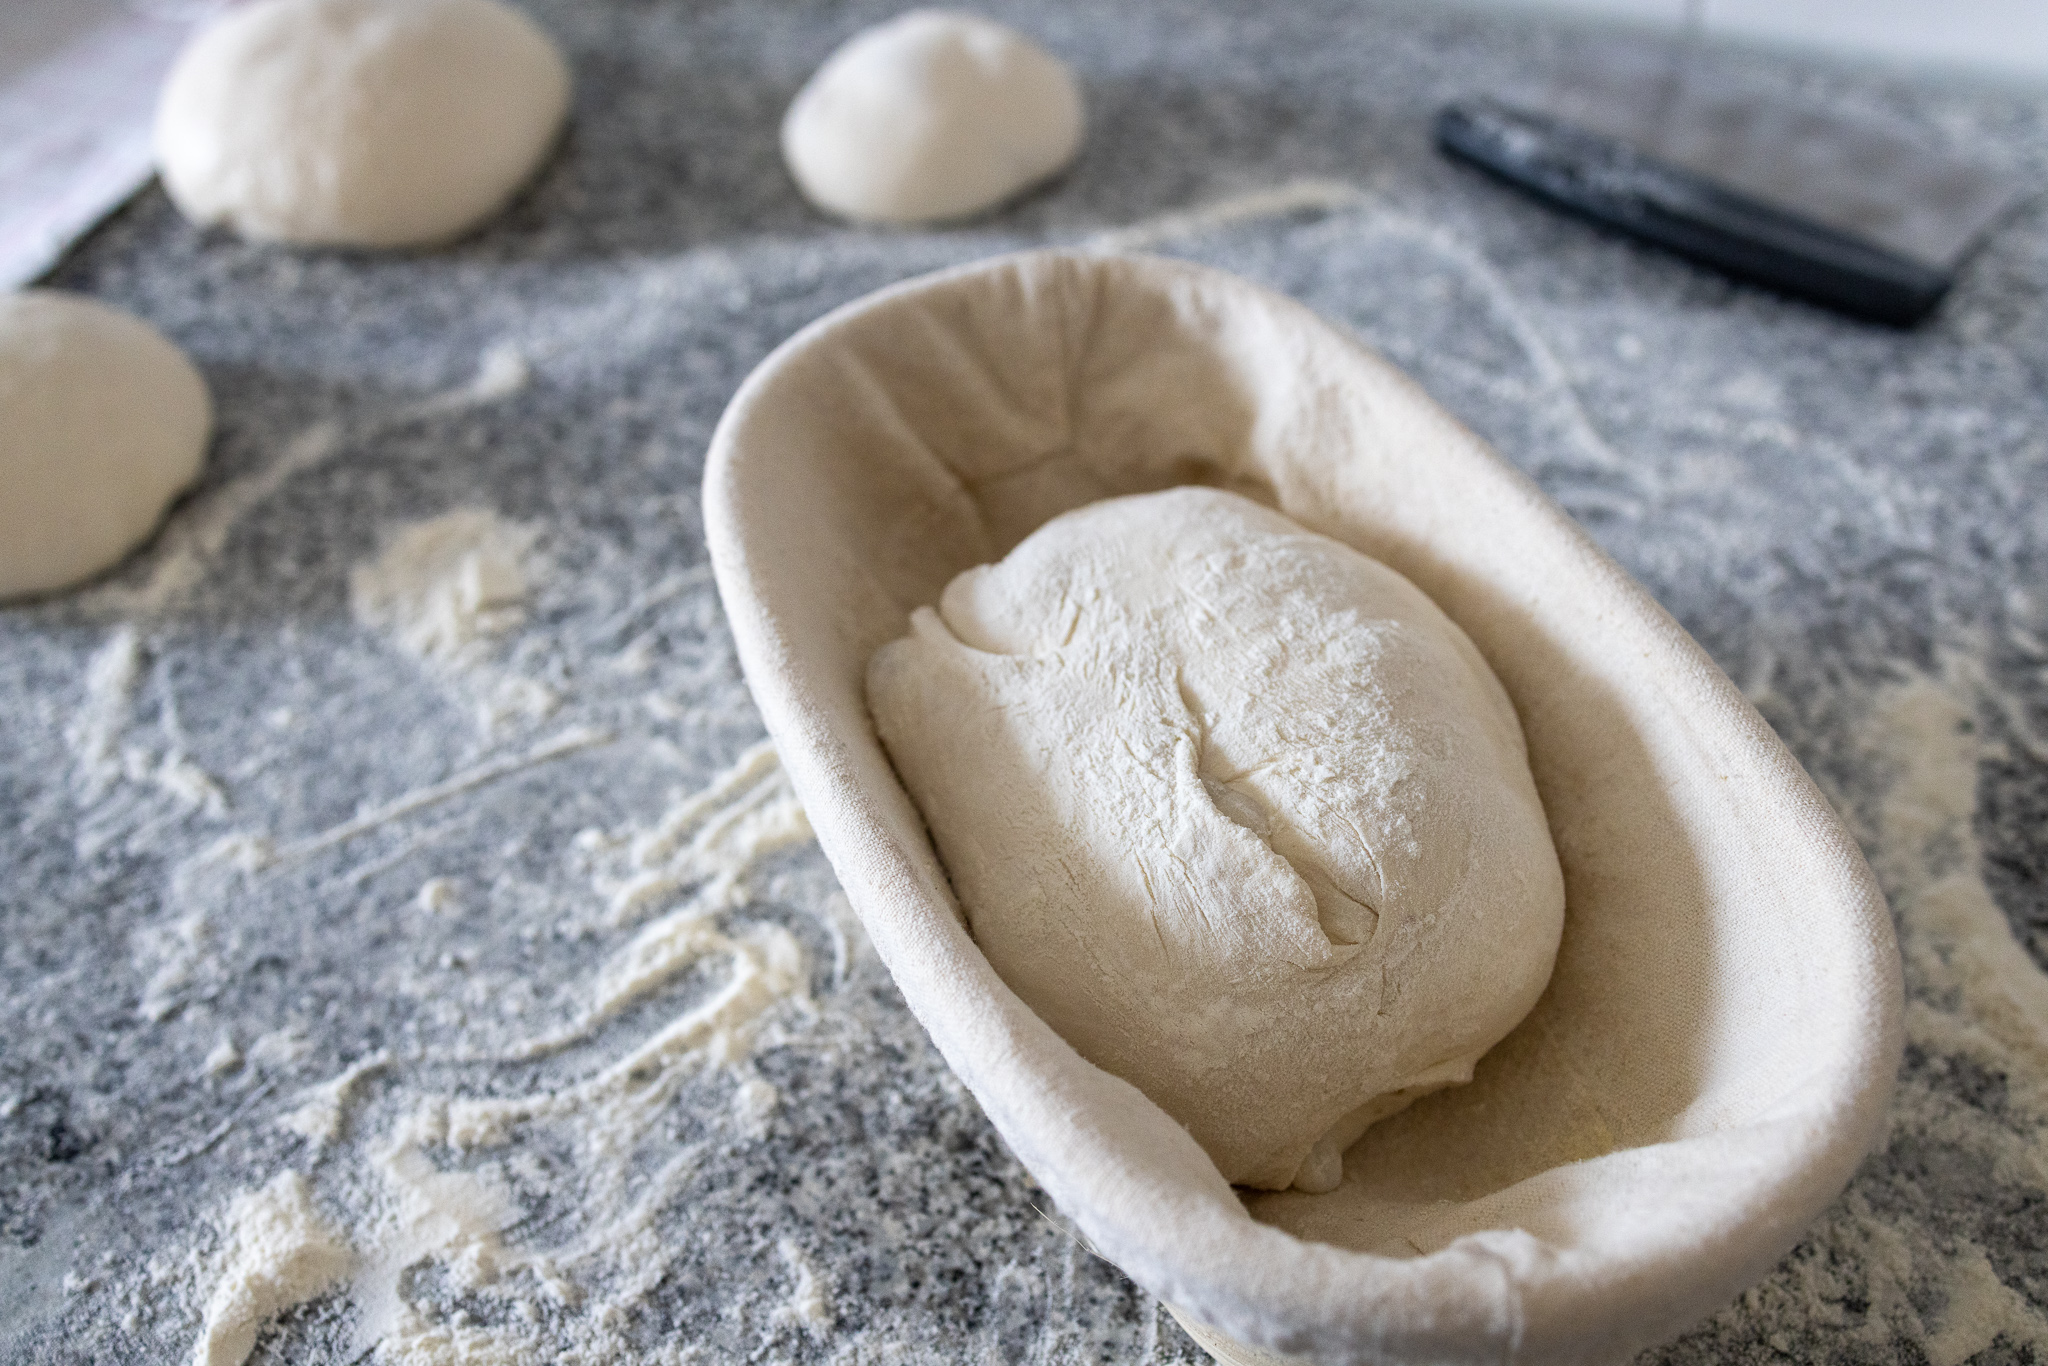
\includegraphics[width=\textwidth]{step-6-prepare-proofing}
  \caption[Step 5 of shaping process]{The shaped dough is ready for proofing
      in the banneton. Note how the seam side is now facing you. The floured
      previous top side is facing downwards.}%
  \label{fig:shaping-prepare-proofing}
\end{figure}

You should have a beautifully shaped dough in front of you now.
The proofing stage is about to start. To simplify later
scoring and to make sure your dough won't stick to your banneton,
apply another flour rub to the dough's surface. This
will dry out the surface and reduce the dough's tendency
to stick to everything.

For the coating, I~recommend using the same flour you used
to make your dough. Rice flour is only recommended if you
want to apply artistic scoring patterns later. It is better
to use more flour than too little flour. Excess flour can be
brushed off later.

Once your dough has been coated, it is ready to be placed on your banneton.
If you do not have a banneton, you can use a bowl
with a kitchen towel inside.

The currently top-facing floured surface will be downwards-facing in your banneton.
By doing so the banneton can be flipped
over before baking, releasing the dough\footnote{The same
applies when making other doughs such as baguette doughs. The floured
surface will always be downwards facing. The dough is then flipped over
once for baking.}.

Proceed and lift the dough with 2 hands from the counter.  Gently rotate it
once and then place the dough in your banneton for proofing\footnote{The seam
    side should now be facing you.  Some bakers like to seal the seam a little
    more. I~did not notice that this improves the dough's strength. As far as
    I~can tell, this only improves the visual appearance of the bottom side of
    the final loaf.}.
If you did everything right, then your dough should look somewhat similar to
the dough shown in Figure~\ref{fig:shaping-prepare-proofing}.  As the last
step of shaping, place a kitchen towel over your banneton or bowl and begin
proofing.

\section{Proofing}

In bread baking, proofing refers to the final rise of dough before baking,
after it has been shaped into a loaf. The chemical reactions and processes
that occur during bulk fermentation and proofing are the same.

By shaping your dough, it has lost some of the air previously generated
throughout the bulk fermentation. The goal of proofing is to inflate
the dough again. A dough without proofing wouldn't offer the same texture
as a properly proofed dough. The proofed dough features a very fluffy
and soft crumb.

There are two proofing techniques. One strategy is to proof the dough
at room temperature whereas the other proofs the dough in the fridge.
Fridge-proofing is also commonly known as retarding.

Some bakers claim that cold-proofing improves the final flavor of the bread.
In all the loaves that I~retarded I~could not tell a difference
in terms of flavor for cold-proofed doughs. The microorganisms work
at a slower rate at colder temperatures. But I~doubt that they alter
their biochemical processes. More research is needed on the topic
of retarding and flavor development.

\begin{flowchart}[!htb]
\centering
  \begin{tikzpicture}[node distance = 3cm, auto]
  \node [decision] (init) {\footnotesize Room temperature proofing?};
  \node [decision, right of=init, node distance=9cm] (retard_bake_decision) {\footnotesize Bake in less than 10 hours from now?};
  \node [block, below of=init, node distance=4cm] (poke) {\footnotesize Poke the dough};
  \node [block, right of=poke, node distance=4cm] (wait_poke) {\footnotesize Wait 15 minutes};
  \node [decision, below of=poke, node distance=3cm] (dent_visible_decision) {\footnotesize Dent still visible after 1 minute?};
  \node [block, right of=dent_visible_decision, node distance=4cm] (bake) {\footnotesize Score and bake};
  \node [block, below of=retard_bake_decision, node distance=3cm] (wait_retard) {\footnotesize Wait 15 minutes};
  \node [block, below of=wait_retard, node distance=3cm] (retard) {\footnotesize Proof in fridge at 4°C (40°F)};
  \node [block, right of=wait_retard, node distance=3cm] (move_to_fridge) {\footnotesize Move dough directly to fridge};
  \path [line] (init) -- node{yes} (poke);
  \path [line] (init) -- node{no} (retard_bake_decision);
  \path [line] (poke) -- (dent_visible_decision);
  \path [line] (dent_visible_decision) -- node{yes} (bake);
  \path [line] (dent_visible_decision) -- node{no} (wait_poke);
  \path [line] (wait_poke) -- (poke);
  \path [line] (retard_bake_decision) -- node{yes} (wait_retard);
  \path [line] (retard_bake_decision) -- node{no} (move_to_fridge);
  \path [line] (wait_retard) -- (retard);
  \path [line] (move_to_fridge) -- (retard);
  \path [line] (retard) -- (bake);
\end{tikzpicture}

  \caption[Sourdough proofing process]{A schematic overview of the different steps of
      the sourdough proofing process. The proofing technique to choose depends
      on your availability and schedule.}%
  \label{fig:proofing-process}
\end{flowchart}

To me, the sole purpose of cold-proofing is its ability to allow you
to better manage the timing of the whole process. Assuming you finished shaping
your dough at 10 pm, chances are you wouldn't want to wait for another
2~hours to proof the dough and then another 1 hour to bake it. In this case,
you can move your dough directly to the fridge after shaping. Your
dough will be proofing overnight in the fridge. Then it can be baked at any time
the following day (there are a few exceptions; more on that later).
This is especially handy for large-scale bakeries that use fridge-proofing
extensively. Some of the doughs are proofed a day before and placed in the fridge.
Early in the morning, they can be baked directly out of the fridge. Within 2
hours they will be ready to sell the first bread to morning customers. If
throughout the day more bread is needed, they simply take some proofed dough out
of the fridge and bake it. The time frame in which you can bake retarded
dough is big. It can be as little as 6~hours later up to 24~hours later.

Assuming you made an overnight dough and your dough is ready in the morning,
the situation might be different. You potentially want to bake the dough directly
for breakfast, or at lunchtime. In this case, you wouldn't want to proof the dough for
another 6~hours in the fridge. Room temperature-proofing is your technique
of choice.

To summarize, choose the technique that works for you depending on your
schedule and availability.

\subsection{Room temperature-proofing}

The easiest and most reliable way to proof your dough is to proof the dough at
room temperature. It is my method of choice if my schedule allows it. This method
works great if you make an overnight dough and then proof it the next
morning.

\begin{figure}[htb!]
  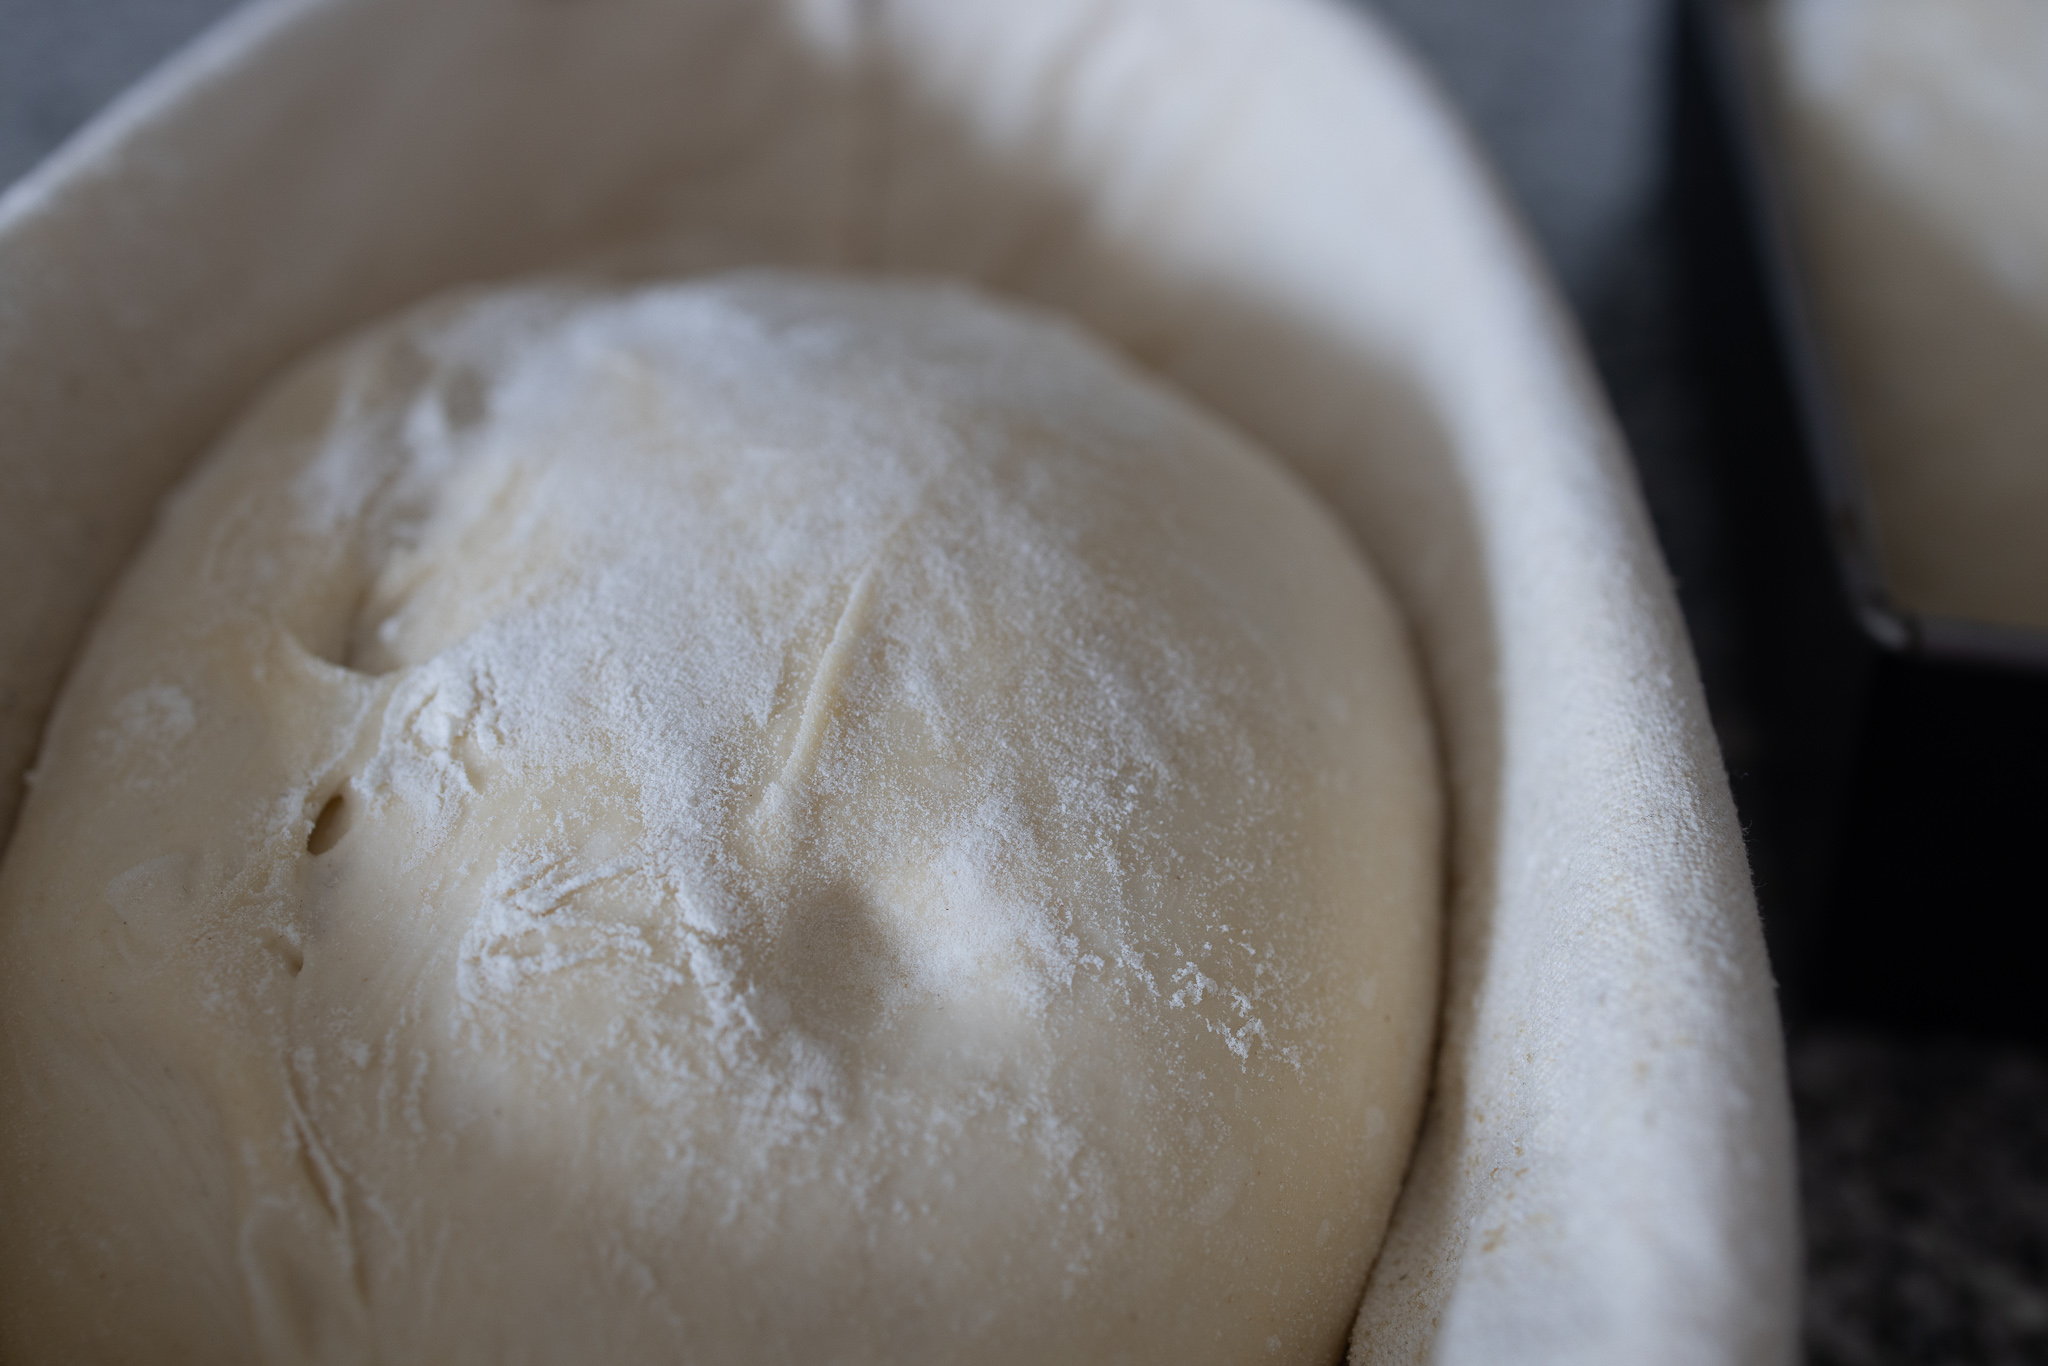
\includegraphics[width=\textwidth]{step-13-finger-poke-test}
  \caption[The finger poke test]{The finger poke test is a very reliable
      method to check if your dough has been properly proofed. If the induced
      dent is still visible one minute later, your dough can be baked.}%
  \label{fig:shaping-finger-poke}
\end{figure}

The time it takes to proof your dough can be anything between 30~minutes and
3~hours. Rather than relying on timing, most bakers use the finger poke test.

Flour your thumb and gently press around 0.5cm up to 1cm deep into the dough.
Try this directly after shaping. You will notice that the created dent will
recover quickly. It will be gone again after 1 minute.

As you proceed with proofing, your dough will fill up with more gas. At the
same time, the dough will become more extensible. Once it starts to reach the
right amount of fluffiness and extensibility, the dent will disappear more slowly.
Once the dough is ready for scoring and baking the dent should still be visible after
1 minute of waiting.

I~recommend performing the finger poke test once every 15~minutes throughout
the proofing stage. Realistically, based on my experience, proofing takes at least
one hour and can sometimes take up to 3~hours. Even at warmer temperatures proofing
has never been faster than an hour for me. As always please take my timings with
a grain of salt and experiment on your own.

Once I~see that the dough is getting close to perfect proofing, I~proceed and
preheat my oven. This way I~don't overproof the dough. You would notice an
over-proofed dough when the dough suddenly becomes very sticky. At the same
time, the dough is likely to collapse during baking and will not spring back.
Generally, it is better to end proofing too early rather than too late.

\subsection{Cold-proofing (retarding)}

The second proofing option is to place your dough inside the fridge for
proofing. This option is great if you do not want to bake the dough
within the next 3~hours.

The dough will initially proof at the same rate as the room temperature dough.
As the dough cools down the rate of fermentation slows. Ultimately at below
\qty{4}{\degreeCelsius} (\qty{40}F) the fermentation comes to a halt\footnote{The actual temperature
depends on the bacteria and yeast you cultivated in your sourdough
starter.}. The dough can rest in the fridge for up to 24~hours. In some
experiments, the dough was still good even 48~hours later. Interestingly,
there is a limit to fridge proofing. I~can only explain this with continuous
fermentation activity at low temperatures.

The hard part is to judge when the dough is finished proofing in your fridge.
The previously mentioned finger poke test does not work on cold dough. Low
temperatures change the dough's elasticity. The dent from the poke test
will never recover.

For this reason, finding the best fridge-proofing time is best done
with an iterative approach. Begin with 8~hours on your first dough,
10~hours on the second, 12~hours on the third, and so on up to 24~hours.
As the temperature in your fridge is typically constant, you have an
environment in which you can rely on timings. Find the ideal proofing
time that works for you.

One additional consideration is the dough's core temperature before
placing it inside the fridge. The warmer your dough is initially
the longer it takes for the dough to cool down. This is an additional
variable to take into consideration when choosing the retarding time.
In summer times when my kitchen is hot, I~choose a shorter fridge-proofing
time compared to winter times when the dough is colder.

A reliable way to ensure consistent proofing is to opt for using a pH
meter. By checking the amount of piled-up acidity you can ensure
each of your doughs has the right amount of acidity. Opt for an iterative
approach and check the pH for multiple proofing times. Find the pH
value that creates the best bread for you. Once you have identified
your perfect pH value you can resort to that number on all following
doughs. See Table~\ref{table:sample-ph-values} for some sample pH values
to follow.

\section{Scoring}

Once your dough is done proofing, it's time to warm up your oven
to around \qty{230}{\degreeCelsius} (\qty{446}{\degF}). The next step is then
to proceed with scoring your dough.

Scoring is done for two reasons. There is functional and decorative
scoring. Functional scoring refers to making a small incision in the dough
through which it rises while baking. If the dough is not scored,
it would likely crack open at the weakest spots where you sealed
the dough after shaping. Decorative scoring can be used to apply
artistic patterns to your dough and make it more appealing. When
you want to apply artistic scoring, it is best to rub your dough
with additional rice flour before scoring. The white rice flour
greatly boosts the contrast of the scoring incisions and thus
makes the final pattern look more visually appealing.

\begin{figure}[htb!]
  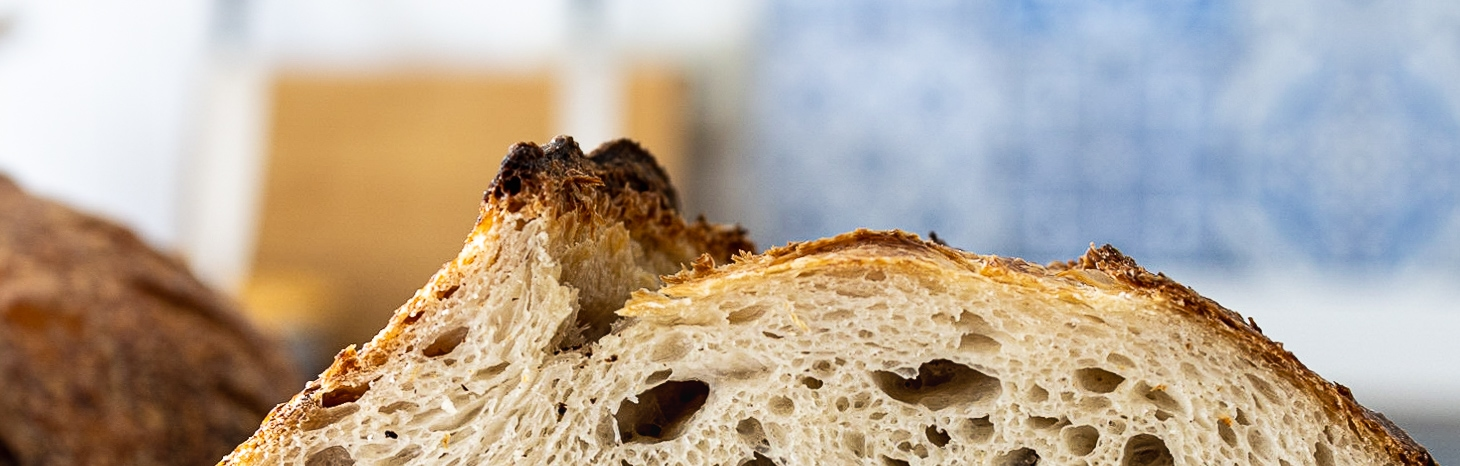
\includegraphics[width=\textwidth]{the-ear}
  \caption[Bread's ear]{The ear is a characteristic that can be achieved on
      wheat sourdough when fermenting and scoring your dough with the perfect
      technique. It offers additional flavor and great texture when eating the
      bread.}%
  \label{fig:the-ear}
\end{figure}

When using a banneton, the dough is flipped over and
placed on an oven rack, tray, stone, steel, or dutch oven. The pros
and cons of the different baking options are covered in the next chapter.
The dough's top side which was previously at the bottom of the
banneton should now be facing you.

\begin{figure}[htb!]
  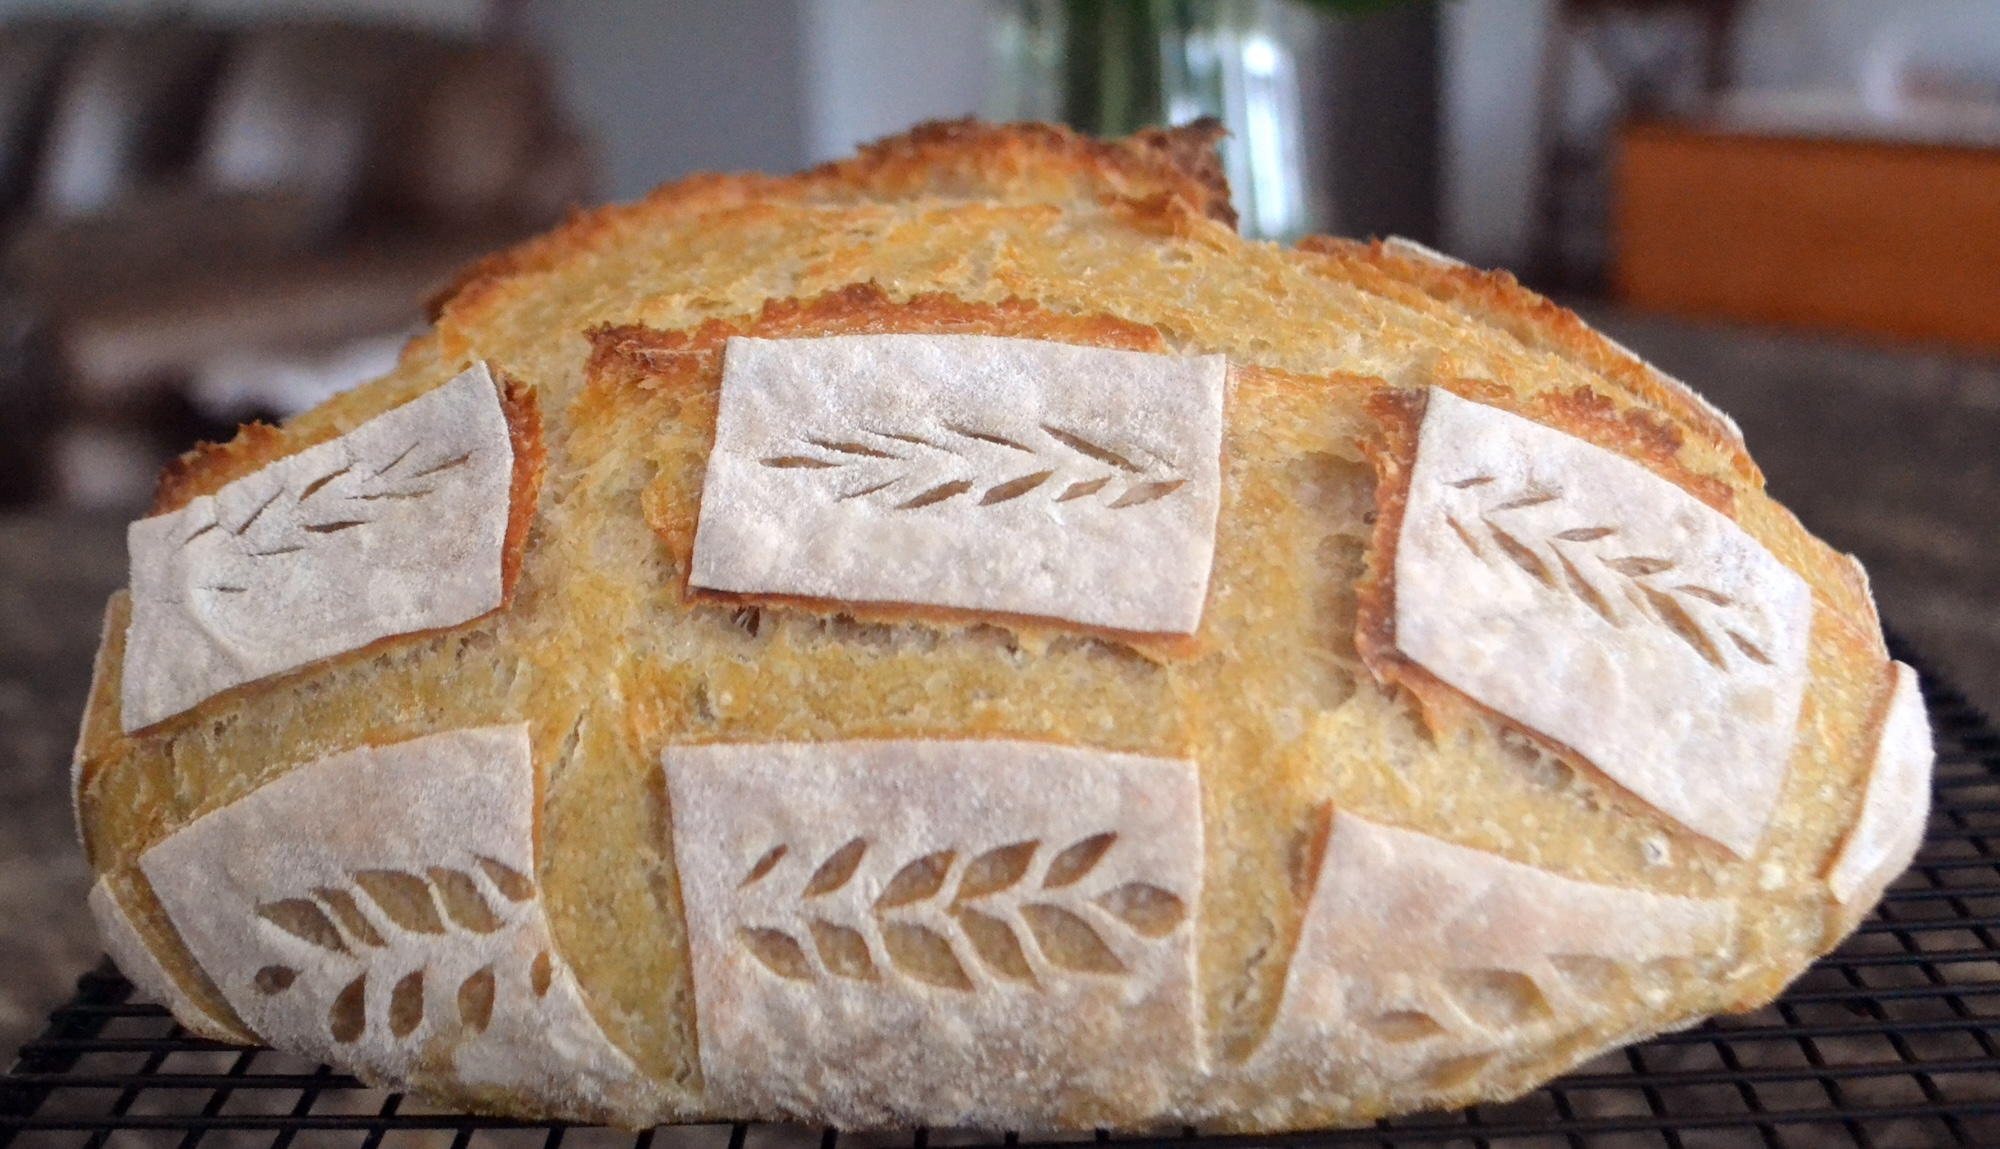
\includegraphics[width=\textwidth]{artistic-scoring}
  \caption[Artistic scoring]{A loaf by Nancy~Anne featuring an artistic
      scoring pattern.  The high contrast was achieved by rubbing the dough's
      surface with rice flour before baking. Her Instagram account
      \texttt{simply.beautiful.sourdough} is specialized to showcase beautiful
      artistic scoring patterns.}%
  \label{fig:artistic-scoring}
\end{figure}

The scoring cut is done at a \ang{45}~angle relative to the dough's
surface slightly off the dough's center. With the \ang{45}~angle cut
the overlaying side will rise more in the oven than the other side.
This way you will achieve a so-called \emph{ear} on the final bread.
The ear is a thin crisp edge that offers intriguing texture
when eating. The thin edge is typically a bit darker after baking
and thus offers additional flavor. In my opinion, the ear turns
a good loaf into a great loaf.

\begin{figure}[htb!]
  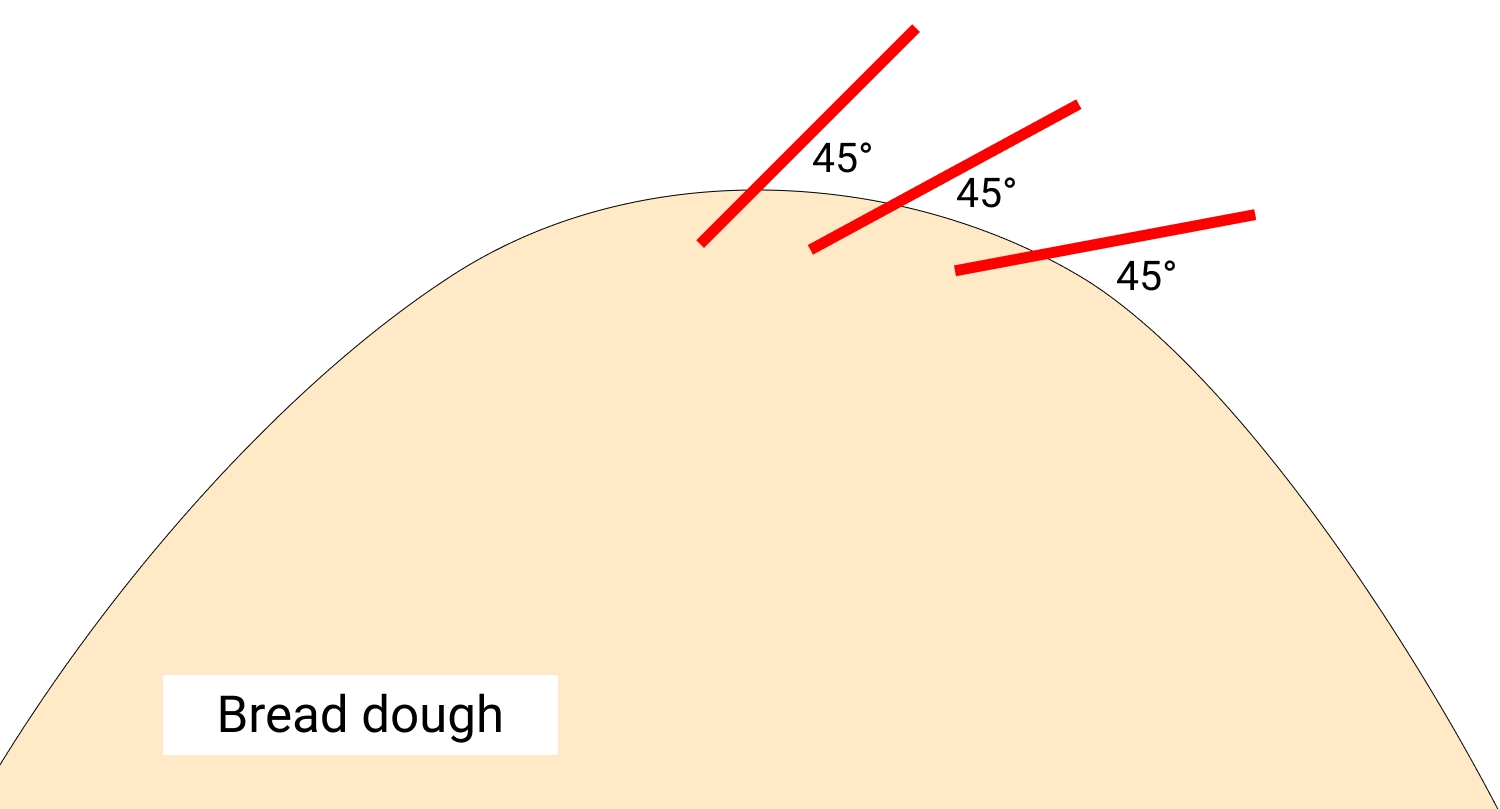
\includegraphics[width=\textwidth]{bread-scoring-angle}
  \caption[Scoring angle]{The \ang{45}~angle at which you score the
      dough is relative to the surface of the dough.  When scoring more towards
      the side, you have to adjust the angle to achieve the ear on your
      bread.}%
  \label{fig:scoring-angle}
\end{figure}

The actual incision is done with a very sharp knife, or better, a razor
blade. You can use the razor blade directly or attach it to a chopstick.
The razor blade offers better flexibility than the sharp knife.
Regardless, the blade should be as sharp as possible. This way when cutting,
the dough is not torn and instead features a clean, non ragged incision.

To simplify scoring, your dough's surface must be dried out a little bit.
This way it is a lot easier to make the incision.
For this reason, it is crucial to rub your dough with a bit of flour
before placing it in the banneton. The dry flour will absorb some of the
moisture of the outer layers of your dough. This is especially important
when working with room temperature-proofed doughs. A cold-proofed dough
is a lot easier to score due to the dough's low viscosity. The room-temperature
dough is a lot harder to score. The scoring incision tears a lot
easier. With a ragged incision, the dough is not as likely to properly
rise in the oven. Chances are you will not achieve the previously mentioned
ear. For this reason, drying out the surface is especially important. Scoring
will become a lot easier.

\begin{figure}[htb!]
  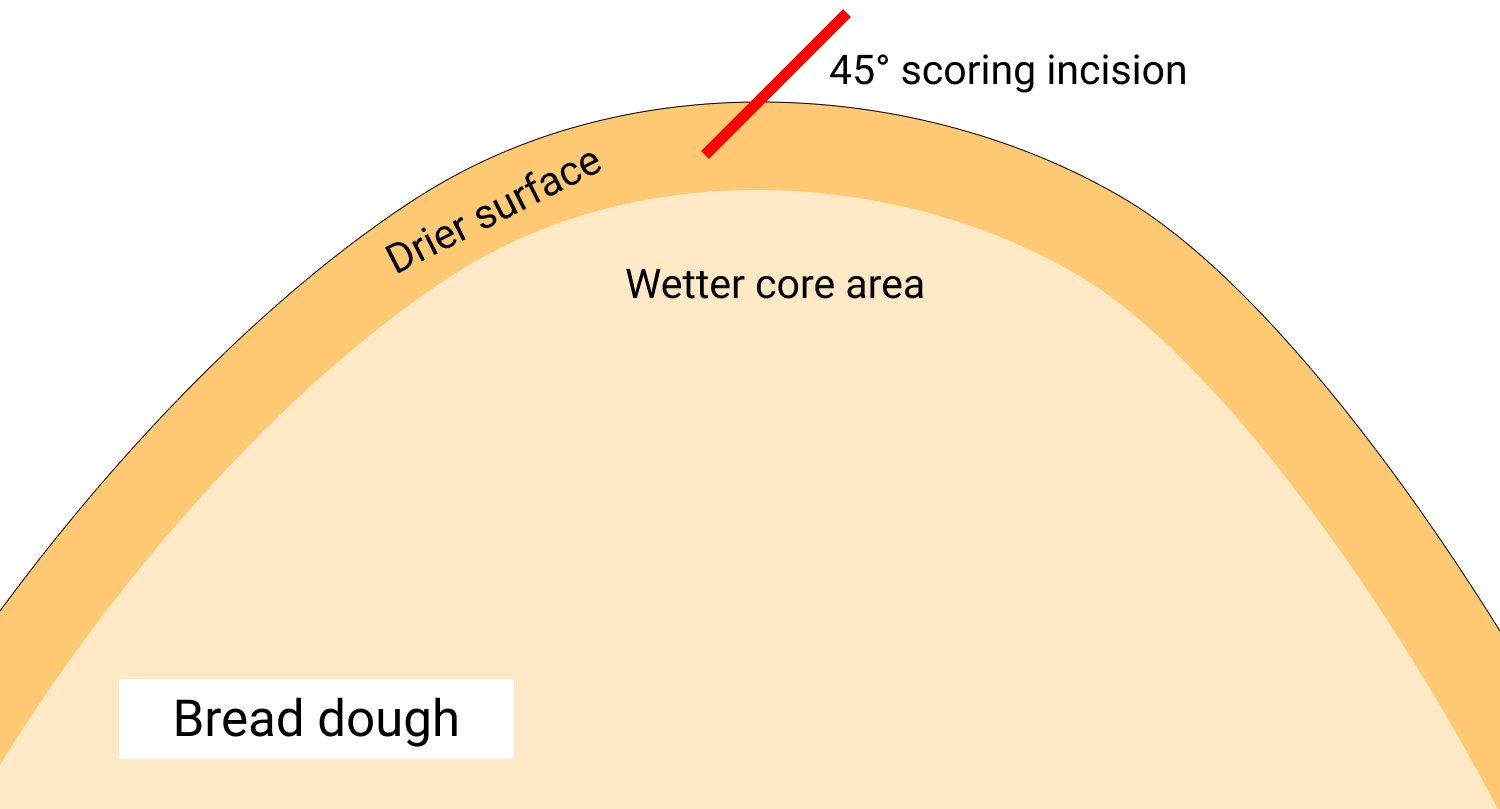
\includegraphics[width=\textwidth]{dry-dough-surface}
  \caption[Drying the dough surface]{By applying flour to your dough's surface
      after shaping, the outer part of the dough dries out a little bit. This
      makes scoring a lot easier as the incision is less likely to tear.}%
  \label{fig:dried-out-dough-scoring}
\end{figure}


Scoring requires a lot of practice. For this reason, I~recommend
practicing making the incision after creating dough strength. The dough
is going to be very wet and sticky. You can use a sharp knife or razor
blade to practice the technique. Wait a few minutes and then round
up the dough again. You can practice this for as long as you like
until you are happy with your technique. After proofing, you only
have a single chance to practice scoring. It's either hit or miss.

An additional trick that can help you to combine the benefits
of room temperature-proofing and easy cold-proofing scoring
is to place your dough in the freezer for 30~minutes before baking.
Once you notice your dough is almost done proofing, move it to the
freezer. The freezer will dry out the dough's surface even further
while also lowering its viscosity, making scoring easier.

Another interesting trick is to bake your dough for 30 seconds without steam.
The hot air will dry out the dough's surface even further and simplify
the scoring technique. Experiment with the timing to identify your personal
sweet spot.
